%% Department of Biostatistics Consulting Report Template
%% Version 2.2
%% Sarah R Haile, 2010.12.14
%% Sina Rüeger, 2012.02.20, 2012.12.06 (for STA490)
%% Eva Furrer, 2013.02.01 (for STA490)
%% Isaac Gravestock, 2014.09.01 (Update for RStudio, knitr)
%% Servan Gr?ninger, 2015.12.23
\documentclass[11pt, a4paper,twoside]{report}\usepackage[]{graphicx}\usepackage[]{color}
%% maxwidth is the original width if it is less than linewidth
%% otherwise use linewidth (to make sure the graphics do not exceed the margin)
\makeatletter
\def\maxwidth{ %
  \ifdim\Gin@nat@width>\linewidth
    \linewidth
  \else
    \Gin@nat@width
  \fi
}
\makeatother

\definecolor{fgcolor}{rgb}{0.345, 0.345, 0.345}
\newcommand{\hlnum}[1]{\textcolor[rgb]{0.686,0.059,0.569}{#1}}%
\newcommand{\hlstr}[1]{\textcolor[rgb]{0.192,0.494,0.8}{#1}}%
\newcommand{\hlcom}[1]{\textcolor[rgb]{0.678,0.584,0.686}{\textit{#1}}}%
\newcommand{\hlopt}[1]{\textcolor[rgb]{0,0,0}{#1}}%
\newcommand{\hlstd}[1]{\textcolor[rgb]{0.345,0.345,0.345}{#1}}%
\newcommand{\hlkwa}[1]{\textcolor[rgb]{0.161,0.373,0.58}{\textbf{#1}}}%
\newcommand{\hlkwb}[1]{\textcolor[rgb]{0.69,0.353,0.396}{#1}}%
\newcommand{\hlkwc}[1]{\textcolor[rgb]{0.333,0.667,0.333}{#1}}%
\newcommand{\hlkwd}[1]{\textcolor[rgb]{0.737,0.353,0.396}{\textbf{#1}}}%
\let\hlipl\hlkwb

\usepackage{framed}
\makeatletter
\newenvironment{kframe}{%
 \def\at@end@of@kframe{}%
 \ifinner\ifhmode%
  \def\at@end@of@kframe{\end{minipage}}%
  \begin{minipage}{\columnwidth}%
 \fi\fi%
 \def\FrameCommand##1{\hskip\@totalleftmargin \hskip-\fboxsep
 \colorbox{shadecolor}{##1}\hskip-\fboxsep
     % There is no \\@totalrightmargin, so:
     \hskip-\linewidth \hskip-\@totalleftmargin \hskip\columnwidth}%
 \MakeFramed {\advance\hsize-\width
   \@totalleftmargin\z@ \linewidth\hsize
   \@setminipage}}%
 {\par\unskip\endMakeFramed%
 \at@end@of@kframe}
\makeatother

\definecolor{shadecolor}{rgb}{.97, .97, .97}
\definecolor{messagecolor}{rgb}{0, 0, 0}
\definecolor{warningcolor}{rgb}{1, 0, 1}
\definecolor{errorcolor}{rgb}{1, 0, 0}
\newenvironment{knitrout}{}{} % an empty environment to be redefined in TeX

\usepackage{alltt}

\usepackage{verbatim}
% \usepackage[vmargin=3cm, hmargin=2cm]{geometry}
\RequirePackage[hyphens]{url}
\usepackage[colorlinks=true,pdftex]{hyperref} 
\PassOptionsToPackage{hyphens}{url}\usepackage{hyperref}
\usepackage{fancyhdr}
\usepackage{color}
\usepackage{amsmath, amssymb}
\usepackage{amsthm} %for proof env
\usepackage{multirow}
\usepackage{colortbl}
\usepackage{longtable}
\usepackage{lscape}
\usepackage{subcaption}


\usepackage[authoryear,round]{natbib}
\usepackage[resetlabels]{multibib}
\newcites{packages}{Software packages} %to cite R packages & software
%\usepackage[backend=bibtex]{biblatex}
\usepackage{xspace}
\usepackage{float}

% Use Palatino (URW Palladio) for most of the text\ldots
%\usepackage[sc]{mathpazo}
\linespread{1.05} 
\definecolor{grey}{rgb}{.95,.95,.95}


% And Arial for the rest
%\usepackage[scaled]{helvet}

%set graphics path
\graphicspath{{./fig/}}

% sans serif caption (added by sina)
%\usepackage[font=sf, labelfont={sf}, margin=1cm]{caption}

% fonts for captions the same as for text
\usepackage{caption}

% DEUTSCH
%\usepackage[german]{babel}
%\usepackage[T1]{fontenc}
%\usepackage[latin1]{inputenc}
\usepackage[utf8]{inputenc}
\usepackage{textcomp} %to write degree symbol °

%Use special macros
%% We load package by package and set package relevant parameters.
% Topics are summarized later
%%%%%%%%%%%%%%%%%%%%%%%%%%%%%%%%%%%%%%%%%%%%%%%%%%%%%%%%%%%%%%%%%%%%%%%%
% helping packages
\usepackage{ifthen}
\usepackage{calc}

%%%%%%%%%%%%%%%%%%%%%%%%%%%%%%%%%%%%%%%%%%%%%%%%%%%%%%%%%%%%%%%%%%%%%%%%

\renewcommand{\baselinestretch}{1.2}
\renewcommand{\textfraction}{0}%0.2     % placement of figures
\renewcommand{\topfraction}{1}%.3
\renewcommand{\bottomfraction}{1}%.3
\renewcommand{\floatpagefraction}{1}%.3
\setcounter{bottomnumber}{3}%1

\textwidth6.3in
\textheight9.7in
\topmargin-45pt
\oddsidemargin-.15in
\evensidemargin.15in
\headsep30pt
\headheight15pt
%\footskip20pt


%%%%%%%%%%%%%%%%%%%%%%%%%%%%%%%%%%%%%%%%%%%%%%%%%%%%%%%%%%%%%%%%%%%%%%%%

\usepackage{color}
\definecolor{fgcolor}{rgb}{0.345, 0.345, 0.345}
\definecolor{shadecolor}{rgb}{.97, .97, .97}
\definecolor{messagecolor}{rgb}{0, 0, 0}
\definecolor{warningcolor}{rgb}{1, 0, 1}
\definecolor{errorcolor}{rgb}{1, 0, 0}
\definecolor{DarkBlue}{rgb}{0,0,0.5451}
\definecolor{DarkGreen}{rgb}{0,0.39216,0}
\definecolor{LightYellow}{rgb}{1,1,.8}
\definecolor{orange}{rgb}{.9,0.3445,0}



%%%%%%%%%%%%%%%%%%%%%%%%%%%%%%%%%%%%%%%%%%%%%%%%%%%%%%%%%%%%%%%%%%%%%%%%
\usepackage{afterpage}
\usepackage{natbib}
\usepackage{upquote}

\usepackage[english]{babel}

%%%%%%%%%%%%%%%%%%%%%%%%%%%%%%%%%%%%%%%%%%%%%%%%%%%%%%%%%%%%%%%%%%%%%%%%%%%%%%%
%% maxwidth is the original width if it is less than linewidth
%% otherwise use linewidth (to make sure the graphics do not exceed the margin)
\makeatletter
\def\maxwidth{ %
  \ifdim\Gin@nat@width>\linewidth
    \linewidth
  \else
    \Gin@nat@width
  \fi
}
\makeatother

\newcommand{\hlnum}[1]{\textcolor[rgb]{0.686,0.059,0.569}{#1}}%
\newcommand{\hlstr}[1]{\textcolor[rgb]{0.192,0.494,0.8}{#1}}%
\newcommand{\hlcom}[1]{\textcolor[rgb]{0.678,0.584,0.686}{\textit{#1}}}%
\newcommand{\hlopt}[1]{\textcolor[rgb]{0,0,0}{#1}}%
\newcommand{\hlstd}[1]{\textcolor[rgb]{0.345,0.345,0.345}{#1}}%
\newcommand{\hlkwa}[1]{\textcolor[rgb]{0.161,0.373,0.58}{\textbf{#1}}}%
\newcommand{\hlkwb}[1]{\textcolor[rgb]{0.69,0.353,0.396}{#1}}%
\newcommand{\hlkwc}[1]{\textcolor[rgb]{0.333,0.667,0.333}{#1}}%
\newcommand{\hlkwd}[1]{\textcolor[rgb]{0.737,0.353,0.396}{\textbf{#1}}}%

\usepackage{framed}
\makeatletter
\newenvironment{kframe}{%
 \def\at@end@of@kframe{}%
 \ifinner\ifhmode%
  \def\at@end@of@kframe{\end{minipage}}%
  \begin{minipage}{\columnwidth}%
 \fi\fi%
 \def\FrameCommand##1{\hskip\@totalleftmargin \hskip-\fboxsep
 \colorbox{shadecolor}{##1}\hskip-\fboxsep
     % There is no \\@totalrightmargin, so:
     \hskip-\linewidth \hskip-\@totalleftmargin \hskip\columnwidth}%
 \MakeFramed {\advance\hsize-\width
   \@totalleftmargin\z@ \linewidth\hsize
   \@setminipage}}%
 {\par\unskip\endMakeFramed%
 \at@end@of@kframe}

\renewenvironment{kframe}{%
 \def\at@end@of@kframe{}%
 \ifinner\ifhmode%
  \def\at@end@of@kframe{\end{minipage}}%
  \begin{minipage}{\columnwidth}%
 \fi\fi%
 \def\FrameCommand##1{\hskip\@totalleftmargin \hskip-0\fboxsep
 \colorbox{shadecolor}{##1}\hskip-0\fboxsep
     % There is no \\@totalrightmargin, so:
     \hskip-\linewidth \hskip-\@totalleftmargin \hskip\columnwidth}%
 \MakeFramed {\advance\hsize-\width
   \@totalleftmargin\z@ \linewidth\hsize
   \@setminipage}}%
 {\par\unskip\endMakeFramed%
 \at@end@of@kframe}

\makeatother

% \newenvironment{knitrout}{}{} % an empty environment to be redefined in TeX

\newenvironment{knitrout}{\setlength{\topsep}{0mm}\setlength{\fboxsep}{4mm}}{} 
\usepackage{alltt}

%%%%%%%%%%%%%%%%%%%%%%%%%%%%%%%%%%%%%%%%%%%%%%%%%%%%%%%%%%%%%%%%%%%%%%%%%%%%%%%%%%%%%%%%%%%%%%%%%%%%%%%%%%%%
% from fancyvrb
\usepackage{fancyhdr}
\usepackage{fancyvrb}
\DefineVerbatimEnvironment{Rcode}{Verbatim}{xleftmargin=2em,fontshape=sl,formatcom=\color{DarkGreen}}
\fvset{listparameters={\setlength{\topsep}{0pt}}}

%%%%%%%%%%%%%%%%%%%%%%%%%%%%%%%%%%%%%%%%%%%%%%%%%%%%%%%%%%%%%%%%%%%%%%%%%%%%%%%%%%%%%%%%%%%%%%%%%%%%%%%%%%%%%
\usepackage{float}
\usepackage{graphicx}
\usepackage[margin=2em,labelfont=bf]{caption}



%%%%%%%%%%%%%%%%%%%%%%%%%%%%%%%%%%%%%%%%%%%%%%%%%%%%%%%%%%%%%%%%%%%%%%%%
\usepackage[pdftex,plainpages=false,pdfpagelabels,pagebackref=true,colorlinks=true,pdfpagemode=UseOutlines]{hyperref}


%%%%%%%%%%%%%%%%%%%%%%%%%%%%%%%%%%%%%%%%%%%%%%%%%%%%%%%%%%%%%%%%%%%%%%%%
% now math stuff and other details...
\usepackage{amsmath,amsthm,amssymb}

\newtheorem{pro}{Property}[chapter]
\theoremstyle{definition}
\newtheorem{des}{Definition}[chapter]
\newtheorem{bsp}{Example}[chapter]
\newtheorem{rem}{Remark}[chapter]

%\newcommand{\widebar}[1]{\overline{#1}}
\newcommand*\widebar[1]{%
  \vbox{%
    \hrule height 0.5pt%     % Line above with certain width
    \kern0.5ex%             % Distance between line and content
    \hbox{%
      \kern-0.1em%           % Distance between content and left side of box, negative values for lines shorter than content
      \ifmmode#1\else\ensuremath{#1}\fi%  % The content, typeset in dependence of mode
      \kern-0.1em%      % Distance between content and left side of box, negative values for lines shorter than content
    }% end of hbox
  }% end of vbox
}
\def\ds{\displaystyle}

\newcommand{\rr}[1]{{\ttfamily\slshape\color{DarkGreen} #1}}

\makeatletter


% clever trick to circumvent potential redefines after loading packages:
% \providecommand{\something}{}  % if it does not exist, it creates it.
%      has same syntax as \newcommand
% \renewcommand{\something}{....}
% TUGboat 29(2)


\makeatletter
%umdefinierung exisitierender befehle
\let\oldH\H
\let\oldL\L
\let\oldO\H
\let\oldS\S
\let\olda\a
\let\oldb\b
\let\oldc\c
\let\oldd\d
\let\oldk\k
\let\oldv\v
\let\oldl\l
\let\oldt\t
\let\oldu\u
\let\oldIJ\IJ
\let\oldP\P
\let\P\relax
\let\oldnorm\|

%\DefineVerbatimEnvironment{CodeInput}{Verbatim}{fontshape=sl}
%\DefineVerbatimEnvironment{CodeOutput}{Verbatim}{}

\def\endrem{\hfill$\clubsuit$\\}
\def\endbibrem{\hfill$\spadesuit$\\}


\renewcommand{\|}{|\!|}         % closer norm
\newcommand{\T}{{}^{\top}}%\newcommand{\T}{{}^{\mathsf{T}}}
\newcommand\code[1]{{\tt#1}}
\DeclareMathOperator{\tol}{T}                       % Tolerance reagion

\def\spam{\code{spam}}
\def\R{{\sf R}}
\def\fields{\code{fields}}


\newcounter{algo}
\newenvironment{algorithm}{%
  \begin{list}{
      (\arabic{algo})
    }{
      \usecounter{algo}
    }%
}{
  \end{list}
}

% some text abbreviation
\newcommand{\GLS}{\text{GLS}}
\newcommand{\RR}{\text{RR}}
\newcommand{\OR}{\text{OR}}
\newcommand{\WLS}{\text{WLS}}
\newcommand{\MLE}{\text{MLE}}
\newcommand{\OLS}{\text{OLS}}
\newcommand{\MAE}{\text{MAE}}
\newcommand{\MAD}{\text{MAD}}
\newcommand{\RMSE}{\text{RMSE}}

\newcommand{\ii}{\text{\i}}

\newcommand{\Bin}{\cB\mathit{\!i\!n}}
\newcommand{\Beta}{\cB\mathit{\!e\!t\!a}}
\newcommand{\Pois}{\cP\mathit{\!o\!i\!s\!s\!o\!n}}
\newcommand{\Exp}{\cE\mathit{\!x\!p}}


\DeclareMathOperator*{\argmin}{argmin}
\DeclareMathOperator*{\argmax}{argmax}
\DeclareMathOperator{\diag}{diag}
\DeclareMathOperator{\diam}{diam}
\DeclareMathOperator{\card}{card}
\DeclareMathOperator{\cov}{Cov}                   
\DeclareMathOperator{\corr}{Corr}                 
\DeclareMathOperator{\var}{Var}                   
\DeclareMathOperator{\trace}{tr}                  
\DeclareMathOperator{\E}{E}                       
\DeclareMathOperator{\P}{P}                       
\DeclareMathOperator{\pred}{p}
\DeclareMathOperator{\vect}{vec}                  
\DeclareMathOperator{\vech}{vech}                 
\DeclareMathOperator{\rank}{rank}                 
\DeclareMathOperator{\e}{e}                       
%\DeclareMathOperator{\cv}{CV}                     
\DeclareMathOperator{\GCV}{GCV}                     
\DeclareMathOperator{\CV}{CV}                     
\DeclareMathOperator{\BLUP}{BLUP}                 
\DeclareMathOperator{\MSE}{MSE}                   
\DeclareMathOperator{\MS}{MS}                   
\DeclareMathOperator{\df}{df}                   
\DeclareMathOperator{\bias}{bias}                   
\DeclareMathOperator{\eig}{eig}                   
\DeclareMathOperator{\Prec}{Prec}
\DeclareMathOperator{\mode}{mode}
\renewcommand{\SS}{\text{SS}}
\renewcommand{\d}{\mathsf{\,d}}

\def\arctanh{\qopname\relax o{arctanh}}  % as in amsopn
\newcommand{\bigo}{\cO}
\newcommand{\lito}{\text{\scriptsize{$\cO$}}}
\newcommand{\cdfPhi}{\itPhi}
\newcommand{\simiid}{\stackrel[]{\text{iid}}{\sim}}
\newcommand{\ml}{_\text{ML}}

\newcommand*{\stack@relbin}[3][]{%
  \mathop{#3}\limits
  \toks@{#1}%
  \edef\reserved@a{\the\toks@}%
  \ifx\reserved@a\@empty\else_{#1}\fi
  \toks@{#2}%
  \edef\reserved@a{\the\toks@}%
  \ifx\reserved@a\@empty\else^{#2}\fi
  \egroup
}%
\renewcommand*{\stackrel}{\mathrel\bgroup\stack@relbin}
\newcommand*{\stackbin}{\mathbin\bgroup\stack@relbin}


% Kalligraphischer Schriftsatz
\newcommand{\cA}{{\cal{A}}}
\newcommand{\cB}{{\cal{B}}} 
\newcommand{\cC}{{\cal{C}}}
\newcommand{\cD}{{\cal{D}}} 
\newcommand{\cE}{{\cal{E}}}
\newcommand{\cF}{{\cal{F}}}
\newcommand{\cG}{{\cal{G}}}
\newcommand{\cH}{{\cal{H}}}
\newcommand{\cI}{{\cal{I}}}
\newcommand{\cJ}{{\cal{J}}}
\newcommand{\cK}{{\cal{K}}}
\newcommand{\cL}{{\cal{L}}}
\newcommand{\cM}{{\cal{M}}} 
\newcommand{\cN}{{\cal{N}}}
\newcommand{\cO}{{\cal{O}}} 
\newcommand{\cP}{{\cal{P}}}
\newcommand{\cQ}{{\cal{Q}}} 
\newcommand{\cR}{{\cal{R}}} 
\newcommand{\cS}{{\cal{S}}} 
\newcommand{\cT}{{\cal{T}}}
\newcommand{\cU}{{\cal{U}}}
\newcommand{\cV}{{\cal{V}}}
\newcommand{\cW}{{\cal{W}}}
\newcommand{\cX}{{\cal{X}}} 
\newcommand{\cY}{{\cal{Y}}}
\newcommand{\cZ}{{\cal{Z}}} 


\newcommand{\IA}{{\mathbb{A}}}
\newcommand{\IB}{{\mathbb{B}}}
\newcommand{\IC}{{\mathbb{C}}}
\newcommand{\ID}{{\mathbb{D}}}
\newcommand{\IE}{{\mathbb{E}}}
\newcommand{\IF}{{\mathbb{F}}}
\newcommand{\IG}{{\mathbb{G}}}
\newcommand{\IH}{{\mathbb{H}}}
\newcommand{\II}{{\mathbb{I}}}
%\newcommand{\IJ}{{\mathbb{J}}}
\newcommand{\IK}{{\mathbb{K}}}
\newcommand{\IL}{{\mathbb{L}}}
\newcommand{\IM}{{\mathbb{M}}}
\newcommand{\IN}{{\mathbb{N}}}
\newcommand{\IO}{{\mathbb{O}}}
\newcommand{\IP}{{\mathbb{P}}}
\newcommand{\IQ}{{\mathbb{Q}}}
\newcommand{\IR}{{\mathbb{R}}}
\newcommand{\IS}{{\mathbb{S}}}
\newcommand{\IT}{{\mathbb{T}}}
\newcommand{\IU}{{\mathbb{U}}}
\newcommand{\IV}{{\mathbb{V}}}
\newcommand{\IW}{{\mathbb{W}}}
\newcommand{\IX}{{\mathbb{X}}}
\newcommand{\IY}{{\mathbb{Y}}}
\newcommand{\IZ}{{\mathbb{Z}}}


% fette griechische kleinbuchstaben
\newcommand{\balpha}{{\boldsymbol{\alpha}}}
\newcommand{\bbeta}{{\boldsymbol{\beta}}}
\newcommand{\bgamma}{{\boldsymbol{\gamma}}}
\newcommand{\bdelta}{{\boldsymbol{\delta}}}
\newcommand{\blambda}{{\boldsymbol{\lambda}}}
\newcommand{\bepsilon}{{\boldsymbol{\epsilon}}}
\newcommand{\bvarepsilon}{{\boldsymbol{\varepsilon}}}
\newcommand{\bzeta}{{\boldsymbol{\zeta}}}
\newcommand{\bfeta}{{\boldsymbol{\eta}}}  %  <----- exception !
\newcommand{\btheta}{{\boldsymbol{\theta}}{}}
\newcommand{\bvartheta}{{\boldsymbol{\vartheta}}}
\newcommand{\biota}{{\boldsymbol{\iota}}}
\newcommand{\bkappa}{{\boldsymbol{\kappa}}}
\newcommand{\bmu}{{\boldsymbol{\mu}}}
\newcommand{\bnu}{{\boldsymbol{\nu}}}
\newcommand{\bxi}{{\boldsymbol{\xi}}}
\newcommand{\bpi}{{\boldsymbol{\pi}}}
\newcommand{\bvarpi}{{\boldsymbol{\varpi}}}
\newcommand{\brho}{{\boldsymbol{\rho}}}
\newcommand{\bvarrhoi}{{\boldsymbol{\varrho}}}
\newcommand{\bsigma}{{\boldsymbol{\sigma}}}
\newcommand{\bvarsigma}{{\boldsymbol{\varsigma}}}
\newcommand{\btau}{{\boldsymbol{\tau}}}
\newcommand{\bvartau}{{\boldsymbol{\vartau}}}
\newcommand{\bupsilon}{{\boldsymbol{\upsilon}}}
\newcommand{\bphi}{{\boldsymbol{\phi}}}
\newcommand{\bvarphi}{{\boldsymbol{\varphi}}}
\newcommand{\bchi}{{\boldsymbol{\chi}}}
\newcommand{\bpsi}{{\boldsymbol{\psi}}}
\newcommand{\bomega}{{\boldsymbol{\omega}}}


% fette griechische grossbuchstaben
\newcommand{\bGamma}{{\boldsymbol{\Gamma}}}
\newcommand{\bDelta}{{\boldsymbol{\Delta}}}
\newcommand{\bTheta}{{\boldsymbol{\Theta}}}
\newcommand{\bLambda}{{\boldsymbol{\Lambda}}{}}
\newcommand{\bXi}{{\boldsymbol{\Xi}}}
\newcommand{\bPi}{{\boldsymbol{\Pi}}}
\newcommand{\bSigma}{{\boldsymbol{\Sigma}}{}}
\newcommand{\bUpsilon}{{\boldsymbol{\Upsilon}}{}}
\newcommand{\bPhi}{{\boldsymbol{\Phi}}}
\newcommand{\bPsi}{{\boldsymbol{\Psi}}}
\newcommand{\bOmega}{{\boldsymbol{\Omega}}}

% italics griechische grossbuchstaben
\newcommand{\itGamma}{{\mathit{\Gamma}}}
\newcommand{\itDelta}{{\mathit{\Delta}}}
\newcommand{\itTheta}{{\mathit{\Theta}}}
\newcommand{\itLambda}{{\mathit{\Lambda}}}
\newcommand{\itXi}{{\mathit{\Xi}}}
\newcommand{\itPi}{{\mathit{\Pi}}}
\newcommand{\itSigma}{{\mathit{\Sigma}}}
\newcommand{\itUpsilon}{{\mathit{\Upsilon}}}
\newcommand{\itPhi}{{\mathit{\Phi}}}
\newcommand{\itPsi}{{\mathit{\Psi}}}
\newcommand{\itOmega}{{\mathit{\Omega}}}



\newcommand{\A}{{\mathbf{A}}}
\newcommand{\B}{{\mathbf{B}}}
\newcommand{\C}{{\mathbf{C}}}
\newcommand{\D}{{\mathbf{D}}}
\newcommand{\bfE}{{\mathbf{E}}}    % \E: expectation
\newcommand{\F}{{\mathbf{F}}}
\newcommand{\G}{{\mathbf{G}}}
\renewcommand{\H}{{\mathbf{H}}}
\newcommand{\I}{{\mathbf{I}}}
\newcommand{\J}{{\mathbf{J}}}
\newcommand{\K}{{\mathbf{K}}}
\renewcommand{\L}{{\mathbf{L}}}
\newcommand{\bfM}{{\mathbf{M}}}
\newcommand{\N}{{\mathbf{N}}}
\renewcommand{\O}{{\mathbf{O}}}
\newcommand{\bfP}{{\mathbf{P}}}  % \P : probability
\newcommand{\Q}{{\mathbf{Q}}}
\newcommand{\bfR}{{\mathbf{R}}}
\renewcommand{\S}{{\mathbf{S}}}
\newcommand{\bfT}{{\mathbf{T}}} % \T transpose
\newcommand{\U}{{\mathbf{U}}}
\newcommand{\V}{{\mathbf{V}}}
\newcommand{\W}{{\mathbf{W}}}
\newcommand{\X}{{\mathbf{X}}}
\newcommand{\Y}{{\mathbf{Y}}}
\newcommand{\Z}{{\mathbf{Z}}}


\newcommand{\0}{{\mathbf{0}}}
\newcommand{\1}{{\mathbf{1}}}
\newcommand{\2}{{\mathbf{2}}}
\newcommand{\3}{{\mathbf{3}}}
\newcommand{\4}{{\mathbf{4}}}
\newcommand{\5}{{\mathbf{5}}}
\newcommand{\6}{{\mathbf{6}}}
\newcommand{\7}{{\mathbf{7}}}
\newcommand{\8}{{\mathbf{8}}}
\newcommand{\9}{{\mathbf{9}}}

\renewcommand{\a}{{\textbf{\textit{a}}}}
\renewcommand{\b}{{\textbf{\textit{b}}}}
\renewcommand{\c}{{\textbf{\textit{c}}}}
\newcommand{\bfd}{{\textbf{\textit{d}}}}  % \d  'dx'
\newcommand{\bfe}{{\textbf{\textit{e}}}}  % \e  l'exponentiel
\newcommand{\f}{{\textbf{\textit{f}}}}
\newcommand{\g}{{\textbf{\textit{g}}}}
\newcommand{\h}{{\textbf{\textit{h}}}}
\newcommand{\bfi}{{\textbf{\textit{i}}}}%\i  complex i, sans 'dot'
\newcommand{\bfj}{{\textbf{\textit{j}}}}
\renewcommand{\l}{{\textbf{\textit{l}}}}
\renewcommand{\k}{{\textbf{\textit{k}}}}
\newcommand{\m}{{\textbf{\textit{m}}}}
\newcommand{\bfn}{{\textbf{\textit{n}}}}
\newcommand{\bfo}{{\textbf{\textit{o}}}}
\newcommand{\p}{{\textbf{\textit{p}}}}
\newcommand{\q}{{\textbf{\textit{q}}}}
\renewcommand{\r}{{\textbf{\textit{r}}}}
\newcommand{\s}{{\textbf{\textit{s}}}}
\renewcommand{\t}{{\textbf{\textit{t}}}}
\newcommand{\bfu}{{\textbf{\textit{u}}}} %\u used in references
\renewcommand{\v}{{\textbf{\textit{v}}}}
\newcommand{\w}{{\textbf{\textit{w}}}}
\newcommand{\x}{{\textbf{\textit{x}}}}
\newcommand{\y}{{\textbf{\textit{y}}}}
\newcommand{\z}{{\textbf{\textit{z}}}}


 

%=======================================
%settings for title page
\usepackage{geometry}
\RequirePackage{helvet}
\renewcommand\familydefault{\sfdefault} 

\geometry{%
  a4paper,
  top=30mm,
  left=25mm,
  right=25mm,
  bottom=24mm,
  headsep=13mm, %26
  footskip=15mm
}


% =======================================
% Personalized layout
\newcommand{\name}{Servan Grüninger}
\newcommand{\mail}{servan.grueninger@gmail.com}
\newcommand{\versiondate}{2017}
\newcommand{\supervisor}{Prof. Dr. Reinhard Furrer (UZH) \& Prof. Dr. Marcel Salathé (EPFL)}
\newcommand{\bigtitle}{Does the Blue Bird Get the Flu?}
\newcommand{\subtitle}{Using Twitter for Flu Surveillance}
% =======================================
% 
% \newcommand{\web}{www.math.uzh.ch/biostat}
\newcommand{\grp}{Master Thesis in Biostatistics}

\newcommand{\inst}{University of Zurich}
% \newcommand{\img}{
\includegraphics[height=17mm, width = 53mm]{gfx/uzh_logo_e_pos}}
\newcommand{\of}{of\xspace}

\newcommand{\HRule}{\rule{\linewidth}{0.5mm}}
\newcommand{\mytitle}[3]{}



%Headers and footers
\fancypagestyle{standard}{
\fancyhf{}
\renewcommand{\footrulewidth}{0.4pt}
\fancyfoot[ce, co]{\thepage}
\fancyfoot[le, lo]{\textrm{\name}}%, \href{\mail}{\textsf{\emph{\mail}}}
\fancyfoot[re, ro]{\textrm{\versiondate}}
\renewcommand{\headrulewidth}{0.4pt}
\fancyhead[ce, co]{}
\fancyhead[le, lo]{\textrm{\grp}}
\fancyhead[re, ro]{\textrm{\inst}}
}

\fancypagestyle{plain}{%
\fancyhf{}%clear header and footer
\renewcommand{\headrulewidth}{0pt}
\renewcommand{\footrulewidth}{0.4pt}
\fancyfoot[LE, RO]{\thepage}
\fancyfoot[LO, RE]{\textrm{\name}}
\fancyfoot[re, ro]{\textrm{\versiondate}}
}


% =======================================
% bibliography
%\bibliographystyle{ims}


% =======================================
% specific options for Sweave:
%   -- saves all produced plots into a subfolder called 'plots'






% =======================================
%change layout for the rest of document

% =======================================
% my latex commands
\newcommand{\prog}[1]{\textsf{#1}}
\newcommand{\pkg}[1]{\texttt{#1}}
\IfFileExists{upquote.sty}{\usepackage{upquote}}{}
\begin{document}


\renewcommand{\baselinestretch}{1.5}\normalfont
\begin{center}
\setlength{\parindent}{0cm}
\bf\Large% 
Does the Blue Bird Get the Flu?\\
Using Twitter for Flu Surveillance
\normalfont



\hrulefill

\vspace*{4cm}

\large
Master Thesis in Biostatistics (STA495)
\vspace*{12mm}

by

\vspace*{12mm}

Servan Grüninger\\
\small 09-737-040\\
\normalfont
\vspace*{4cm}

supervised by

\vspace*{1cm}

Prof. Dr. Reinhard Furrer\\
Prof. Dr. Marcel Salathé (EPFL)

\vfill

Zurich, 2017
\end{center}
\renewcommand\familydefault{\rmdefault}\normalfont%
%\renewcommand{\baselinestretch}{1.0}\rm 
%set numbering to roman 
\setcounter{page}{0}
\pagenumbering{roman}
\thispagestyle{empty}
\cleardoublepage

%\cleardoublepage

\pagestyle{standard}
%\mytitle{\bigtitle}{\subtitle}

%\hrule
%\pagebreak

\begin{abstract}
Coming soon...
\end{abstract}

\thispagestyle{empty}
\cleardoublepage

\renewcommand{\abstractname}{Acknowledgements}
\begin{abstract}
I would like to thank my two supervisors, Prof. Dr. Reinhard Furrer and Prof. Dr. Marcel Salathé for their academic guidance and critical feedback as well as for the intellectual freedom I was allowed to experience. I thank the Digital Epidemiology lab and its members for free coffee, entertaining group meetings, and stimulating conversations - I'll be back! And I thank my fiancée for taking the time to my rants about malfunctioning code-snippets and error-message-conundrums.
\end{abstract}

\thispagestyle{empty}
\cleardoublepage

% \maketitle
\tableofcontents
\cleardoublepage


\chapter{Introduction}
\label{ch:intro}
\setcounter{page}{0}
\pagenumbering{arabic}
We all know it and we all hate it: The common flu. What may be a mere nuisance for some, can have deadly consequences for others. Every year, between 112'000 and 275'000 patients in Switzerland seek medical care because of influenza-like symptoms, several hundred of which eventually succumb to the disease \citep{bag_lagebericht_2017}. in the U.S., tens of thousands of people die from the flu each year and hundreds of thousands need to be hospitalised \citep{rolfes_estimated_2016}.

However, these numbers represent just the tip of the proverbial ice-berg. Studies have shown that only a minority of the people suffering from influenza or influenza-like symptoms actually seek medical care \citep{goff_surveillance_2015}. In addition, both the Centers for Disease Control and Prevention (CDC) as well the Swiss Federal Office of Public Health only recommend patients to seek medical care if they belong to a risk group or if they show strong symptoms \citep{bag_grippe_2016,cdc_flu_2017}.

This puts traditional influenza surveillance methods, which are usually based on data from healthcare providers acting as sentinels, at a certain disadvantage, because they are more likely to catch the more severe flu cases while underestimating the overall magnitude of the flu. Also, traditional influenza surveillance systems such as ``Sentinalla" in Switzerland \citep{bag_influenza_2017, sentinella_2017} or the ``U.S. Outpatient Influenza-like Illness Surveillance Network" (ILINet) in the USA \citep{cdc_surveillance_2016} only publish their reports with a lag of one to two weeks due to the time it takes to gather and aggregate the available information from the surveillance sentinels.

Hence, novel methods to complement traditional epidemiological information might be needed in order to make influenza surveillance faster and more exhaustive. Luckily, the flu provides researchers with an excellent starting point to test new surveillance methods, due to the following reasons: 

\begin{description}
\item [Reliable data are available] Most high-income countries have well-established Influenza surveillance systems which provide reliable data sources that can be used as ``gold standard" with which the performance of new methods can easily be compared.
\item [Spatio-temporal analysis possible] Influenza leads to recurring epidemics each year all over the world, providing researchers with a vast amount of data to work with.
\item [No stigma attached] Influenza is ``socially accepted", in that Influenza patients are not stigmatised and it is not taboo to talk openly about it (in fact, getting sick with the flu is a very common content of small talk and news articles)
\item [Relevant for public health ] Even though the flu is common, it is far from harmless. As outlined above, the flu poses a serious threat to the health of hundreds of thousands of people in Switzerland alone. Hence, better surveillance method would allow for better preventive and therapeutic measures.
\item [Large body of pre-existing research] Partially due to the reasons outlined above, there exists extensive research about the prevention and treatment of the flu as well as about its etiology, transmission paths, pathophysiology, and virological characteristics. These information serve as excellent basis for epidemiological research
\item [Thriving research community] Many researchers are working on understanding, preventing, and combatting the flu on different levels, offering ample opportunities for collaborations.
\end{description}

\section{Complementary epidemiology}
Epidemiologists have always used a wide range of genetic, population and environmental information to study the transmission and propagation of diseases---from simple counts of disease incidences, mortality or birth tables, and patient histories up to vast cohort studies, sophisticated disease models, and intricate clinical trials \citep{rothman2012epidemiology,koepsell2014epidemiologic}. The epidemiologist's goal is not only to discover where and when a disease occurs, but also why it does so and through which mechanisms. Hence, it should not come as a surprise that the advent of powerful genetic screening techniques, sophisticated algorithms, and cheap computing power have added a lot of new weapons to the scientific arsenal of the ``disease detectives" \citep{bailey2005introduction, khoury_transforming_2013, gardy_real-time_2015}---additions that are sorely needed to keep up with the ever-changing disease landscape.

Nowadays, epidemiological work is decidedly different in two particular ways: First, non-communicable diseases are the primary cause of life-years lost in high-income countries and are on the rise world-wide \citep{lozano_global_2013}. Second, infectious diseases can spread faster than ever before thanks to increased social and spatial mobility on a global scale \citep{hufnagel_forecast_2004}. 

For both challenges, however, novel epidemiological methods are rising to the task. They can help to track down the underlying causes of non-communicable diseases as well as improve the speed and efficiency of disease surveillance methods in order to keep up with emerging epidemics and even pandemics. In this regard, digital data sources appear to be especially promising to complement established epidemiological work \citep{salathe_digital_2012, simonsen_infectious_2016}.

\section{Digital epidemiology}

In the digital age, everybody leaves traces. And thanks to the vast amount of digital footprints each one of us leaves behind, digital data sources do not have to be medical in nature in order to be epidemiological useful. ``Digital epidemiology" can offer epidemiological insights that are very different from traditional surveillance systems and public health infrastructure. More importantly, data sources such as web queries, social networking sites, online news articles, or mobile devices and other wearables have the great advantages of being internationally available and accessible, offering fine-grained geospatial location of the users (or patients) and often allow for instantaneous feedback \citep{salathe_digital_2012}. 

For example, Google tried to use search queries in order to predict the spread and the intensity of the flu in certain countries \citep{ginsberg_detecting_2009}. Retrospective analysis of Google search queries and online media reports showed that these data sources could have been used to detect the Ebola epidemic of 2014/2015 quicker and with more sensitivity \citep{anema_digital_2014, milinovich_role_2015}. And finally, Wikipedia page views proved to be reliable predictors to model the epidemiology of such different diseases as dengue fever, influenza, cholera, HIV/AIDS, or tuberculosis \citep{generous_global_2014}. 

Other services such as ``Health Map" aggregate search engine queries, online news reports, official information from national and international health agencies as well as user eyewitness reports in order to keep track of a wider range of disease outbreaks all over the world \citep{brownstein_surveillance_2008,freifeld_healthmap:_2008}. Finally, there exist a vast range of participatory disease surveillance system, such as ``FrontlineSMS", ``Usahidi", ``GeoChat", ``Asthmapolis", ``Outbreaks Near Me",``Influenzanet", ``FluTracking",``Reporta", ``Dengue na Web", ``SaludBoricua", or ``Flu near you", which use SMS, voice messages, smartphone apps, web forms, or e-mail in order to collect data from and disseminate epidemiological information to afflicted populations \citep{freifeld_participatory_2010,chunara_flu_2013,wojcik_public_2014,chunara_estimating_2015}. In addition, these forms of ``participatory epidemiology" can also help in adding social and economic context to health-related data, defining the research goals and questions, improving the work-flow, or synthesising heterogenous sources of data \citep{bach_participatory_2017,liu_assessing_2017}.

And it does not stop with digital data alone. Many of the approaches outlined above can be combined with and extended by other biologically or clinically relevant data such as high-throughput sequence data, clinical visits, pharmaceutical prescriptions, or clinical symptoms, in order to allow for a more accurate description of the mechanisms of disease spread, the pathogens involved, and the treatments administered \citep{ray_network_2016}.

For the scope of this thesis, I am focusing on one particularly potent source of information: social media data.

\section{What can ``Larry the Bird" tell us about the flu?}
Social media offers the possibility to directly measure a user's sentiments and behaviours via his posts and interactions with other users---information that can be highly valuable from an epidemiological point of view. If somebody is suffering from the flu, her behaviour undoubtedly changes: She behaves more lethargicly, stays in bed, and might complain about her symptoms in the presence of family, friends, or work colleagues. Even people on Twitter or Facebook can exhibit ``disease symptoms" which can be diagnosed. A tweet, in which somebody is complaining about having fever, joint aches, and a cough can be a tell-tale sign of the flu. Similarly, somebody who tweets that all his colleagues were absent from work due to the flu, gives researchers precious and above-all fast warning about an incoming flu wave.

Given that social media is often used to share information about one's personal well-being and/or feeling and takes up an increasing amount of time of many people \citep{bauer_timeonline_2016,scott_time_2017,asano_socialmediatime_2017}, it is to be expected that behavioural changes due to a disease can also be detected by analysing the social media behaviour of the people afflicted. Either because said people are explicitely informing their peers about their current affliction or because the frequency or other implicit aspects of their social media behaviour changes. All these changes ca, in theory, be detected on the population level if researchers get access to data sets that are large enough.

However, using social media for epidemiological surveillance is deeply hampered by one crucial fact: Most social media plattforms do not offer access to user's profiles. The profiles of most social media users are either completely inaccessible to the public (e.g. Whatsapp, Snapchat, FB-Messenger) or only accessible if the user allows it (Facebook, Instagram). But even if profiles are publicly available, they are often not easily accessible and aggregatable for research purposes due to the strict rules of the application programming interfaces (APIs) provided by the respectiv companies.

``Larry the Bird", as Twitter's trademark mascot is affectionately called by its creators \citep{rehak_twitterbird_2014}, is a notable exception to this. Due to the ease-of-access to the Twitter-API as well as due to the fact, that tweets often contain a direct expression of sentiment of some sort, researchers can gain access to millions of tweets sent out every day \citep{twitter_annual_2017}. The source of information is so rich, in fact, that it has spawned a variety of studies in wide range of disciplines, such as political science \citep{tumasjan2010predicting,tumasjan2011election,stieglitz2012political,newman2016tracking}, business \citep{swani2014should,chae2015insights}, economics \citep{bollen2011twitter,bollen2011modeling,zhang2012predicting,sul2014trading}, sociology \citep{poblete2011all,himelboim2013birds,mccormick2015using}, communication science \citep{zhao2009and,marwick2011tweet,himelboim2013birds,hermida2013journalism}, psychology \citep{chen2011tweet,golbeck2011predicting,qiu2012you,eichstaedt2015psychological,braithwaite2016validating}, nutrition science \citep{widener2014using,vidal2015using, abbar2015you}, or medicine \citep{salathe2013dynamics,love2013twitter,nwosu2014social,adrover2015identifying,eichstaedt2015psychological,mowery2017feature}, even though studies from the computer and information sciences studies are clearly in the majority \citep{lee2013real,zimmer2014topology,steiger2015advanced}. 

Hence, it seems straightforward to use Twitter data for epidemiological purposes as well and to fit a model using the content of those tweets as independent variables and the official influenza data as dependent variable.

There is one catch, however: This approach is prone to overfitting, i.e. to picking up signals that do not indicate that the user has the flu, but that are caused by other, unrelated characteristics, which just happen to correlate with, for example, the flu season. Google Flu Trends \citep{ginsberg_detecting_2009} initially fell prey to this kind of overfitting, linking search terms such as ``High School Basketball" to flu disease state---just because the basketball season happened to be in winter which unsurprisingly coincided with the flu season. The Google researchers tried to root out these kind of correlations in order to improve the performance of their algorithms, but eventually had to admit defeat to their daunting task: The huge data masses coupled with changes of user behaviour, external influences from media reports, and the constant adaptions of Google's search algorithm itself created too much noise to allow for reliable flu predictions \citep{olson_reassessing_2013,butler_when_2013,lazer_parable_2014} Eventually, Google Flu Trends was discontinued in summer 2015 as a publicly available service, but the data are still accessible to and used by researchers all around the world \citep{GFT_nextchapter_2015}.

Google Flu trends was a pioneering attempt to use online data to make predictions and despite its (temporary?) failure, it provided researchers with many insights into the promises and perils of using big online data for epidemiological purposes. However, the main problem when using large data sets to infer flu states still remains: How to prevent overfitting if the set of independent variables (e.g. the tweets) is in the billions, while your dependent variables (the official flu information) is in the thousands?

One approach to mitigate this problem is to restrict the relevant tweets to those, which clearly indicate that the user or somebody in her surroundings fell sick to the flu. If somebody tweets: ``stuffy nose, headache and fever---\#flu sucks!" or ``nobody at work - everybody's taking a \#flu leave", then these tweets show a clear presence of a flu infection---either within the tweeter herself or within the people surrounding her. Hence, we can use these tweets to get an estimate of the amount of Twitter users that are currently tweeting about the flu or influenza like symptoms---and thereby of the distribution of flu in the areas where the tweeters are located at.

However, even with the powerful methods from natural language processing, the identification of tweets that indicate disease state (as opposed to general awareness of the flu, for example) is not trivial. There are several very promising methods to extract epidemiologically relevant data from tweets and creating descriptive or predictive models from them. These methods include simple keyword ratios \citep{lampos_tracking_2010}, partial-differential equations \citep{wang_regional_2016}, linear regression models \citep{culotta_towards_2010}, autoregressive models \citep{achrekar_predicting_2011,paul_twitter_2014,paul_worldwide_2015}, support vector machines \citep{paul_you_2011}, probabilistic topic models \citep{paul_you_2011}, sentiment detection \citep{aramaki_twitter_2011}, and semantic text analysis \citep{lamb_separating_2013}. However, most of them still depend on some sort of correlation with official data from public health authorities, making them again prone to overfitting---up to the point that even seemingly irrelevant tweets about zombies can ``predict" flu outbreaks almost as good as tweets containing clinically relevant information \citep{bodnar_validating_2013}. Also, it has been shown that media reports can have a substantial influence on Twitter users' behaviour and thus on the content of their tweets---thereby creating a ``news bias" in the Twitter models \citep{aramaki_twitter_2011}.

It would be prudent then, to validate any keywords that might indicate disease state by comparing them with the true disease state of the tweeter. Since it is implausible to do so with the roughly 319 million of worldwide users who were active on a monthly base by the end of 2016---or even with the 69 million monthly active users in the U.S. \citep{twitter_annual_2017}---we need to aim for a smaller subset.

This is what \cite{bodnar_ground_2014} have done. They built a flu classification model on tweets from users of which they knew the disease state up to the temporal resolution of a month. That is, they had the possibility to build their model knowing which one of the observed Twitter users were sick and which were not within a specific month. Hence, they did not only correlate tweet content with population-level, but could directly assign a Twitter user's timeline with his or her disease state. 

However, this Twitter flu classifier (see Section~\ref{sec:on_the_ground} for details) has only been trained and tested on a very small data set so far. Hence, the first goal of this thesis is to assess the validity of the classifier using 2.8 billion geotagged tweets collected from users on the U.S. mainland over the course of four years (Chapter~\ref{ch:results}) and to make suggestions on how its performance might be improved (Chapter~\ref{ch:discussion}).

\chapter{The challenge of reproducibility}
\label{ch:reproducibility}
An important part of daily research practice is the evaluation and interpretation of other scientist's work. To do so, we mainly rely on information from scientific publications. With the plethora of new articles being published every day and with the increasing difficulty that even high quality journals have when it comes to ensuring the reproducibility of the experiments described in their articles, it is important that researchers know how to critically judge and evaluate papers in order to extract the necessary information they need without being led on the wrong track. 

However, while everybody seems to believe that reproducibility is important, nobody seems to agree on what it exactly is. Hence, talks, papers and discussions about reproducibility are often rife with opportunities for misunderstandings: Some see reproducibility already achieved if a single confirmatory study shows the same overall effect as an exploratory study, others contend that a finding has only been reproduced if several independent studies could show the very same results as the experiment that is supposed to be replicated. In the following, I will give a quick overview over current challenges with regard to reproducibility and also explain how reproducibility plays a role in my thesis. 

\section[To replicate or to reproduce?]{To replicate or to reproduce? Why semantics matter}
\label{sec:replicate}
One of the major sources of confusion in the discussion about (methods) reproducibility is its distinction from replicability (or ``results reproducibility"). Many scientific articles tackling the so-called ``reproducibility crisis" \citep{casadevall_reproducible_2010,prinz_believe_2011,begley2012drug,begley_six_2013,begley2015reproducibility,freedman_economics_2015,aarts2015estimating,baker2016there,baker2016reproducibility,crotty_reproducible_2017,nosek_reproducibility_2017} actually have the issue of replication at heart \citep{schooler2014metascience,stroebe_alleged_2014,kullmann2015biomedicine,maxwell_is_2015,earp_replication_2015,camerer_evaluating_2016,loken_measurement_2017}. So, what is the difference, then?

For \cite{peng_reproducible_2009}, the replication of scientific studies hinges on ``independent investigators, methods, data, equipment, and protocols" in order to evaluate the claims made in said study. However, replicating studies costs time and money and is sometimes neither feasible nor desirable. Nevertheless, ``there is a need for a minimum standard that can fill the void between full replication and nothing." Aiming for reproducibility, defined as the verification of published results and conducting alternative analyses using ``the data sets and computer code [$\dots$] made available to others", could provide such a minimal standard. 

In other words, \cite{peng_reproducible_2009} sees reproducibility given if one can recreate the same results, statistical analyses, tables, and figures as those reported in the original study---not by recollecting the data and rewriting the code, but by using the very same data and code source used by the authors of the study that is supposed to be reproduced. Replication, however, depends on the ability to recreate the same results by independently collecting and evaluating the relevant data.

\cite{cacioppo_social_2015} offer very similar definitions. For them, ``reproducibility refers to the ability of a researcher to duplicate the results of a prior study using the same materials and procedures as were used by the original investigator", i.e. without collecting new data. Replicability, on the other hand, ``refers to the ability of a researcher to duplicate the results of a prior study if the same procedures are followed but new data are collected".

These distinctions have also been adopted by the American Statistical Association, which calls a study reproducible, ``if you can take the original data and the computer code used to analyze the data and reproduce all of the numerical findings from the study". Replicability is defined as ``the act of repeating an entire study, independently of the original investigator without the use of original data (but generally using the same methods)" \citep{broman_recommendation_2017}.

However, \cite{kenett2015clarifying} differentiate between repeatability, reproducibility, and replicability and point out that the nomenclature can vary in meaning across different fields. They suggest ``that these terms can be clarified by considering the intended generalisation of the study", since all three terms ``are aimed at assuring generalizability, but the generalizability is typically of different types". Within this framework, a repeatable finding can be recreated by keeping every aspect of the original study or analysis constant (including exactly the same methods, codes, locations, experimentors etc.); reproducible findings can be recreated by different researchers in different locations, but by using the methods and data sources from the original study; and replicable findings can be recreated by different researchers in different locations with different (i.e. recollected) data and sometimes by using different methods, too. For example, the PDF-version of this thesis can be rebuilt by running the corresponding RNW-file (repeatability), while the findings described therein shoulb be reproducible by using the data and codes provided in the Github-repository (reproducibility) or even by recollecting the data and rewriting the codes (replicability). In other words, repeatable research is least and replicable research is most generalisable.

Finally, \cite{goodman_what_2016} point out that the concept of reproducible research originally emerged in the computational sciences with a clear-cut definition, namely to ``permit the reader of a paper to see the entire processing trail from the raw data and code to figures and tables", even though, nowadays, ``a wide range of issues [are] subsumed under the rubric of reproducibility: design, reporting, analysis, interpretation, and corroborating studies (that is, replication)". However, instead of upholding the existing, but muddled distinction between repeatability, reproducibility, and replicability, they offer a new terminology in order to subsume everything under the concept of reproducibility. That is, they differentiate between methods reproducibility, results reproducibility, and inferential reproducibility. 

Methods reproducibility corresponds to the most common interpretation of reproducibility, namely ``the ability to implement, as exactly as possible, the experimental and computational procedures, with the same data and tools, to obtain the same results." Results reproducibility corresponds to replicability and is ``the production of corroborating results in a new study, having followed the same experimental methods". Inferential reprodudicibility, however, is different from the concepts described so far and refers to ``the drawing of qualitatively similar conclusions from either an independent replication of a study or a reanalysis of the original study".

I believe that distinction given by \cite{goodman_what_2016} is the most straightforward and exhaustive categorisation of different forms of reproducibility. Even the concept of repeatability can be subsumed under this categorisation, namely as an especially stringent case of methods reproducibility. Most importantly, however, this categorisation makes it clear that methods, results, and inferential reproducibility can occur independently from each other, something that is often forgotten in the discussions about reproducibility. In particular, methods reproducibility can be fulfilled even though results and inferential reproducibility are absent---e.g. if a finding based on Twitter user data can be perfectly recreated using the original raw data and codes, but fails replication when collecting data from a different set of Twitter users. The same holds true for results reproducibility, which can exist independently of methods reproducibility---e.g. if the raw data and code of the original study are not provided, but replication is possible by recollecting the data using the methods described in the study---and inferential reproducibility---e.g. if the original results can be replicated but still warrant a different interpretation because of theoretical or methodological discrepancies. Finally, inferential reproducibility can be fulfilled even in the absence of methods and results reproducibility---e.g. when the raw data and code of the original study are missing, while the replication of the study based on the described methods shows an attenuated (or exarcebated) effect with the same directionality as the original study.

For the remainder of this thesis I will therefore adopt the definitons of \cite{goodman_what_2016} and distinguish between methods, results, and inferential reproducibility, respectively.

\section{Ensuring reproducibility: easier said than done}
(Results) reproducibility is often called the ``hallmark" \citep{aarts2015estimating,munafo_manifesto_2017} or ``bedrock" \citep{casadevall_reproducible_2010} of science. After all, what good are scientific findings if they are only valid for the time and place they were originally created? Not much, if we ought to believe the most fervent harbingers of scientific doom.

In fact, the inability to reproduce or replicate many key scientific findings in various fields of research such as drug development \citep{prinz_believe_2011,begley2012drug}, cancer research \citep{nosek_reproducibility_2017}, social psychology \citep{aarts2015estimating}, behavioural economy \citep{camerer_evaluating_2016}, and biological research \citep{freedman_economics_2015,vogt_authorization_2016} have spurred many heated scholarly discussions and led to an exponential increase of the number of papers revolving around the issue \citep{goodman_what_2016}, but it should be noted that the overall body of scientific literature is also increasing exponentially \citep{bornmann2015growth}. So, one could say that studies revolving around or involving reproducibility are just trying to keep up with the avalanche of new articles being published each year.

The discussion does not remain within the realms of academia, either, but has already spilled into the pages and websites of mass media outlets, causing a deluge of articles that are further fuelling the discussion about the ``reproducibility crisis" \citep{lehrer_truth_2010,carey_psychology_2015,carey_scrutiny_2015,achenbach_many_2015,achenbach_reproducibility_2015,yong_psychology_2016,engber_broken_2016,baker_crisis_2016,econ_try_2016,feilden_most_2017,belluz_cancer_2017,meyer_fix_2017}.

It should be noted, however, that (results) reproducibility is neither a necessary nor a sufficient criterion for good science. There are many areas of science (e.g. evolutionary biology, paleontology, geology, climatology astronomy), which make empirical claims about the world based on good scientific practice, but which still fail to be reproducible---simply because it is impossible to replicate dinosaurs marching on earth, vulcanoes erupting, or suns exploding, to just name a few examples \citep{dfg_reproduzierbarkeit_2017}. Many of these disciplines should strive for methods and inferential reproducibility, but they cannot be blamed for failing the test for results reproducibility. 

In experimental research, however, the lack of results reproducibility must give raise to much more concern, even though it should not come as a surprise either. Practices such as multiple comparisons, data mining, $p$-hacking, selective outcome reporting, or hypothesising after the results are known (HARKing), can hamper all three forms of reproducibility and regularly occur in daily research even without the researchers exhibiting any nefarious motivations \citep{goodman_what_2016}. In addition, cognitive and methodical biases such as confirmation, hindsight, framing, or belief bias, and selection, reporting, attrition, recall, or observer bias, respectively, can hamper all three forms of reproducibiliy as well and are commonplace in scientific practice \citep{munafo_manifesto_2017}.

But even when following every methodological, statistical, and scientific rule to the book in order to boost reproducibility as much as possible, findings can be non-reproducible---at least with regard to results and inferential reproducibility---thanks to the standard null hypothesis testing framework, an unfortunate methodological hybrid between the hypothesis testing concept of R. A. Fisher on one hand and the one of Neyman--Pearson on the other \citep{amrhein_earth_2017}. Within this framework, researchers pit their own hypothesis against the Null hypothesis by conducting a significance test, which reveals the probability of receiving a result that is at least as extreme as the one the researchers have received---under the assumption that the Null hypothesis is true. This probability (the $p$-value) is than compared with an arbitrarily defined threshold (e.g. 0.05), either leading to the verdict that the findings are significantly different from the Null ($p < 0.05$) or not significant enough ($p >= 0.05$) for the Null to be rejected. Thus, even under perfect condition without no scientific misconduct whatsoever, we would still expect that 5 \% of all tests against true Null hypotheses turn out to be (falsely) significant. 

This, in combination with publication bias (the preferential publication of statisticallly significant findings in scientific journals) and the inherent uncertainties of scientific research leads to a strong over-representation of false positive research findings in the scientific literature \citep{ioannidis_why_2005}, thereby hampering results reproducibility. And even if the Null hypothesis has been rejected correctly, inferential reproducibility can still be an issue, because scientists often use the rejection of the Null as a sign of support for their alternative hypothesis---even though a significance test is not enough to tell whether this alternative hypothesis is more or less likely to be true than the Null hypothesis. To this, additional information, statistical testing, and inferential reasoning is necessary.

\section{Putting emphasis on methods reproducibility}
As outlined above, ensuring reproducibility is a daunting task that can only be tackled by a multitude of measures and joint efforts from researchers and research institutions. 

Nevertheless, individual researchers can ensure to improve the reproducibility of their own work by following good scientific and statistical practices. Regarding this, I strongly believe that an emphasis on methods reproducibility is the most efficient way to improve overall reproducibility in research, since it provides other researchers with a valuable starting point for their own scientific endeavours.

However, even methods reproducibility remains a challenge that should not be underestimated. As \cite{banks_reproducible_2011} notes: ``Most [research papers] do not come with code or data, and even if they did, I expect a careful check would find discrepancies from the published paper. The reasons for this are innocent: code written by graduate students is continually tweaked and has sketchy documentation. The exact data cleaning procedures are not perfectly remembered when the final version of the paper is written, or may be muddled by miscommunication among multiple authors. And even if a conscientious researcher provided a full description of every cleaning step, every model fitting choice, and all aspects of variable selection, the resulting paper would be so long and tedious that no doubt the foolish editor would demand that it be shortened."

Even in the best of worlds, scientific research cannot follow the textbook of good scientific practice. Still, efforts to improve (methods) reproducibility is paramount to the prolonged reliability of scientific findings. This is especially true for epidemiology in general and digital epidemiology in particular. Epidemiologists aggregate data from different sources such as health agencies, patient reports, or clinical trials, transform them in various ways, and build intricate models based on these aggregations and transformations. In addition, digital epidemiology tries to combine these data with additional sources of information such as billions of Twitter messages, geolocation and sensor data from mobile and tracking devices, or insights from health, fitness, or nutrition apps. 

One important aspect of ensuring reproducible research are detailed and complete reports on the experimental and statistical procedures, the study design, potential confounders, techniques, and methods used, study protocols, statistical designs and further important elements that might be necessary to fully reproduce a scientific finding \citep{kass_ten_2016}. Also, it is of paramount importance that researchers publish data and code as complete and accessible as legally and ethically possible and provide clear and concise descriptions of their work flow \citep{peng_reproducible_2006}.

In the spirit of the issues raised above, this thesis serves a second and third important goal: It is the attempt to test some findings from \cite{bodnar_data_2015} for reproducibility as well as to ensure methods reproducibility for this thesis itself. In addition, the first goal, outlined in Chapter~\ref{ch:intro} and consisting in the validation of the Twitter flu classifier from \cite{bodnar_ground_2014}, can be regarded as an attempt in reproducibility as well, namely results and inferential reproducibility. Hence, the data, analyses, and discussions presented in the following chapters will focus on the methods, results, and inferential reproducibility of the findings from \cite{bodnar_ground_2014} and \cite{bodnar_data_2015}.

\section[On the ground validation of online diagnosis]{On the ground validation of online diagnosis with Twitter and medical records}
\label{sec:on_the_ground}
In their study, conducted during the 2012-2013 Influenza season, \cite{bodnar_ground_2014} analysed the tweeting behaviour of a group of 104 students from the Pennsylvania State University, of which they also had received medical records from the university's health services, telling whether a participant was sick with the flu during a given month or not.

The researchers collected a total of 37'599 tweets from the 104 accounts mentioned above (``seed accounts") as well as 30'950'958 tweets from the 913'082 accounts that were connected to those seed accounts (either by following one of them or by being followed by one of them). They then proceeded to divide the tweets from the seed accounts into two categories: tweets that were sent during a month in which the user was sick on one hand and all other tweets on the other. Out of the 37'599 tweets in the data set, a total of 1609 tweets from 35 users were sent in a month in which their authors were sick.

They then screened the tweets in both categories for the occurrence or absence of a set of keywords \{flu, influenza, sick, cough, cold, medicine, fever\}. The predictive power of these seven words were then tested by applying five different classification methods: J48 (a Java implementation of the C4.5 algorithm), naive Bayes, logistic regression, Naive Bayes, random forest, and support vector machine (SVM). All classification methods failed to reliably correlate the keywords with a Twitter user's disease status (see Figure~\ref{fig:ROC_classification_seed}).

In a second step, the researchers also applied simple bag-of-words techniques to identify relevant keywords, namely by finding the 12'393 most common keywords, ranking them according to their predictive power with regard to Influenza and finally choosing the top 10, 100, or 1000 keywords on this ordered list. The predictive power of the keywords (and thus the ordering of the list) was calculated by classifying the users as either being ``sick" or ``healthy" in a given month and then comparing said classification with the real disease status. The classification was again done using the five methods mentioned above, whereas the naive Bayes classifier performed best with a classification accuracy of 89.72\% and an area under the curver (AUC) of 0.8544 when using the top 100 keywords (see Figure~\ref{fig:ROC_classification_seed}).

\begin{figure}[htbp!]
  \centering
    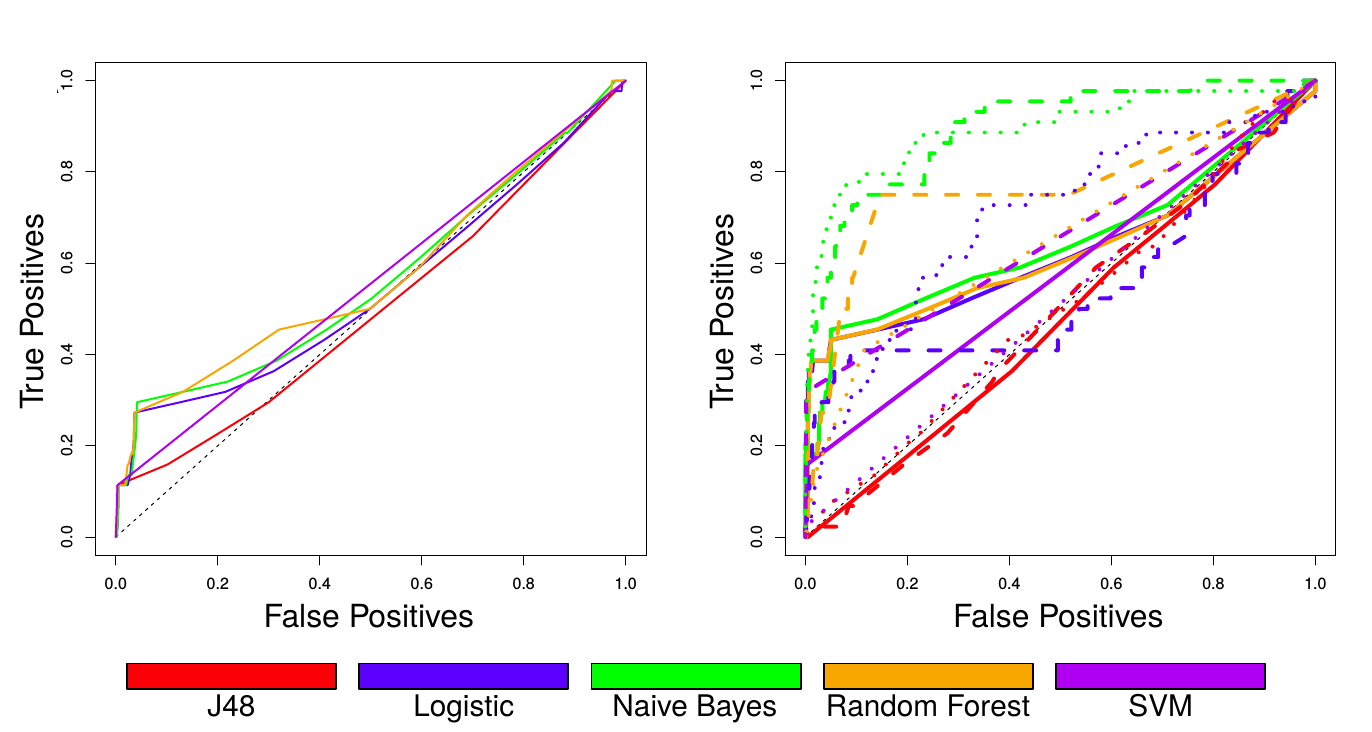
\includegraphics[width=.9\textwidth]{01_ROC_classification_seed.png}
  \caption{The receiver operating characteristic (ROC) of classifiers that use hand chosen key words (left) and algorithmically chosen keywords (right) to determine if an individual is ill. The top 10 (solid line), 100 (dashed line), and 1000 (dotted line) were selected as features. Taken from \cite{bodnar_ground_2014}.}
  \label{fig:ROC_classification_seed}
  \end{figure}

This model has its limitations as well, though: It was based on a very small data set consisting of only 104 Twitter accounts generating a total of 37’599 tweets during the study period. Out of this sample, 35 users fell sick during the study period and generated a total of 1609 tweets in the month in which they were sick. Furthermore, all Twitter users stemmed from the same state (Pennsylvania) and belonged to approximately the same socio-economic group (young students of the Pennsylvania State University). Hence, one would assume that their tweeting behaviour might be different from that of the average Twitter use. In addition, the exact time of disease of the Twitter users is not known. Due to privacy concerns, the researchers were limited to know in which month a specific Twitter user was diagnosed with the flu. Finally, the model was built based on the tweeting behaviour and medical records of only one flu season (2011--2012). All these points either reduce the models' temporal resolution or add a considerable amount of bias to it.

Hence, it is necessary to test the performance of the naive Bayes classifier described above for different cities and states and compare the results with reliable epidemiological data. In his dissertation, \cite{bodnar_data_2015} performed such tests on the level of counties, states, and the complete U.S. mainland.

To do so, he applied the classifier to the tweets of each user within a 4-week sliding window with a one-day step-size. ``The classifier assigns a score to the day where the sliding window begins based on the tweets the user has posted within the window. For example, when the sliding window first encounters a user’s tweet that says `I am getting sick with the flu', the classifier will heavily lean toward her being sick. Later, the user may tweet `I am no longer sick' which will give a strong signal that the user is no longer sick which will tend to outweigh the user’s previous “sick” tweet even if they both occur in the same window. Of course, it is rare that such strong signals are in the data, so the classifier is built on an amalgamation of many weaker signals—mentioning going to a party as not-sick signal, for example---which, while weaker, are more prevalent. We chose a step size of one day in order to increase the temporal granularity of the classifier. Users that are inactive for more than 30 days are not included for any analysis during that time window."

Bodnar applied the algorithm in the above-described fashion to a set of 15'560'328 users who sent a total of 2'732'174'105 geotagged tweets between March $3^\textit{rd}$ 2011 to March $4^\textit{th}$ 2015. Note that tweets from users who tweeted less than 10 times during this period as well as tweets that could not be attributed to a specific state on the U.S. mainland were discarded. However, the total number of tweets analysed was not given in any of the documentations available to me. 

In a next step, Bodnar created a Kermack--McKendrick SIR model based on the results of the classifier \citep{martcheva2015introduction}:
\begin{align}
\frac{dS}{dt} = -SI\beta, \qquad \frac{dI}{dt} = -SI\beta - I\gamma, \qquad \frac{dR}{dt} = I\gamma. label{eq:0}
\end{align}
$S$, $I$, and $R$ represent the relative frequencies of susceptible, exposed, and recovered individuals, respectively, whereas $\beta$ and $\gamma$ are the transition probabilites from being susceptible to having the disease and from having the disease to recovering from it, respectively. To determine the values of $\beta$ and $\gamma$, Bodnar fitted the SIR model based on the data from the Twitter classifier to the official influenza-like illness (ILI) rates from the Centers for Disease Control (CDC) in Atlanta using a multi-grid search method. Note that estimates about flu prevalence are usually made using ILI rates as basis, not confirmed flu cases (see Section~\ref{sec:comparison_cdc} for more details.)

Values for $\beta$ and $\gamma$ were chosen such that the corresponding SIR model minimised the residual sum of squares (RSS):
  \begin{align}
\text{RSS} = \sum_{t}(I_{\gamma, \beta}(t)-I_{\text{CDC}}(t)). \label{eq:1}
  \end{align}
Here, $t$ denotes the time in weeks, while $I$ denotes the percentage of people showing ILI symptoms based on the SIR model ($I_{\gamma, \beta}$ and the official CDC data ($I_{\text{CDC}}$), respectively. By doing so, he calculated the optimal values of $\beta$ and $\gamma$ for each flu season as well as for the whole study period combined (see Table~\ref{tab:nationalparams}). 

\begin{table}[htbp!]
\centering
\caption{National best-fit parameters for each year from the CDC's data (white) and Twitter data (grey); taken from \cite{bodnar_data_2015}.}
\begin{tabular}{l l l l l}

 Year & \(\gamma\) & \(\beta\) & RSS\\ \hline
& 0.1732 & 0.1749  & 0.0001047   \\ 
 {\multirow{-2}{*}{ 2011-2012 }}  & \cellcolor{grey}0.1176  & \cellcolor{grey}0.1195  & \cellcolor{grey}0.0001323  \\ \cline{2-4}
  {\multirow{2}{*}{ 2012-2013 }}& 0.7715 & 0.9626 & 0.0009402   \\ 
   & \cellcolor{grey}0.7317  & \cellcolor{grey}0.9020 & \cellcolor{grey}0.0009492   \\ \cline{2-4}
  {\multirow{2}{*}{ 2013-2014 }}& 0.6054 & 0.7288   & 0.0003114   \\ 
   & \cellcolor{grey}0.6046 & \cellcolor{grey}0.7264 & \cellcolor{grey}0.0003026  \\ \cline{2-4}
  {\multirow{2}{*}{ Combined }}& 0.6998 & 0.8225  & 0.003719   \\ 
   & \cellcolor{grey}0.6765  & \cellcolor{grey}0.7935  & \cellcolor{grey}0.003252   \\ 
\end{tabular}
\label{tab:nationalparams}
\end{table}

Note that in \cite{bodnar_data_2015} it is written that an optimal $S(0)$ was also estimated using the multi-grid search method. However, in the R-code provided to me $S(0)$ was simply defined as $1-I(0)$, where $I(0)$ is the relative number of Twitter users classified as ``sick" during the first week of the time window the SIR-model was built on.

Based on the values given in Table~\ref{tab:nationalparams}, he could then calculate yearly ILI estimates for the flu seasons of 2011--2012, 2012--2013, and 2013--2014 (see Figure~\ref{fig:cdc_fit_bodnar_thesis_SIR}). In addition, he fitted an autocorrelation model using the results from the Twitter base model and the official CDC data: 
  \begin{align}
I_{\text{full}}(t + 1) = a \cdot I_{\text{CDC}}(t - 1) + b \cdot I_{\text{CDC}}(t) + c \cdot I_{\text{Twitter}}(t) + d. \label{eq:2}
  \end{align}
Here, $t$ denotes the time in weeks, $I_{\text{CDC}}$ depicts the official ILI percentages from the CDC (lagged by two and one weeks, respectively), and $I_{\text{Twitter}}$ denotes the ILI percentages received from the Twitter base model (Bodnar, personal communication). It is as of yet unclear whether the ``Twitter base model" is supposed to consist of the raw results from the Twitter classifier or contains these raw results combined with additional information. However, Bodnar confirmed that the ``Twitter base model" is indeed supposed to contain the raw output from the Twitter classifier (personal communication). However, I was not able to retrieve the model paramaters $a$, $b$, and $c$, since I only received a file with the model results, but not the paramater specifications.

\begin{figure}[htbp!]
  \centering
    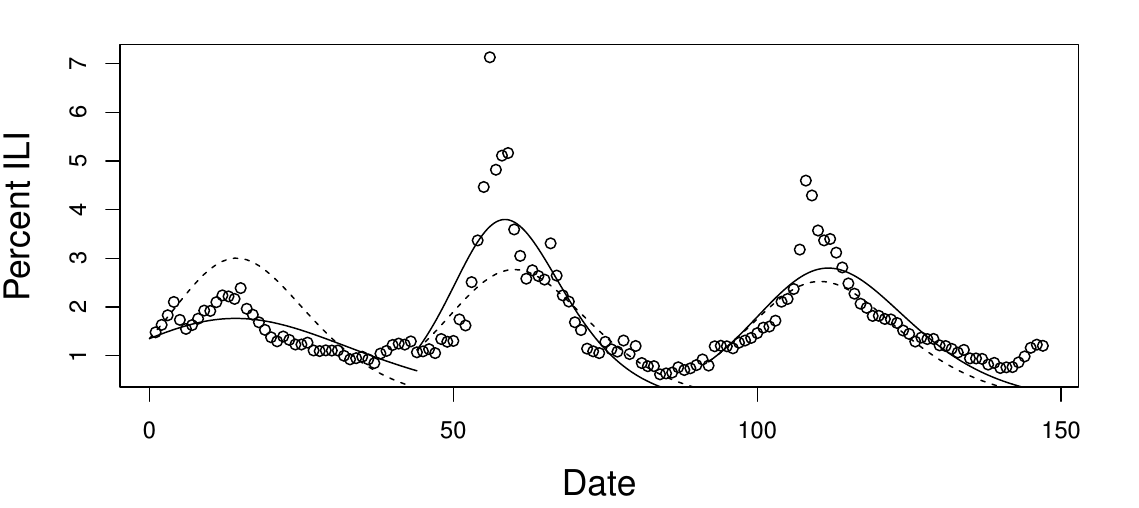
\includegraphics[width=1\textwidth]{02_todd_bodnar_SIR.png}
  \caption{The CDC's estimates (circles) of influenza rates for a three year period compared to the best fit SIR models from the Twitter data using combined (dashed line) or yearly (solid line) parameters. The discontinuities stem from recalculating the SIR models for each year with the ILI rates from the Twitter classifier as a starting point for each year. From \cite{bodnar_data_2015}.}
  \label{fig:cdc_fit_bodnar_thesis_SIR}
  \end{figure}

\begin{figure}[htbp!]
  \centering
    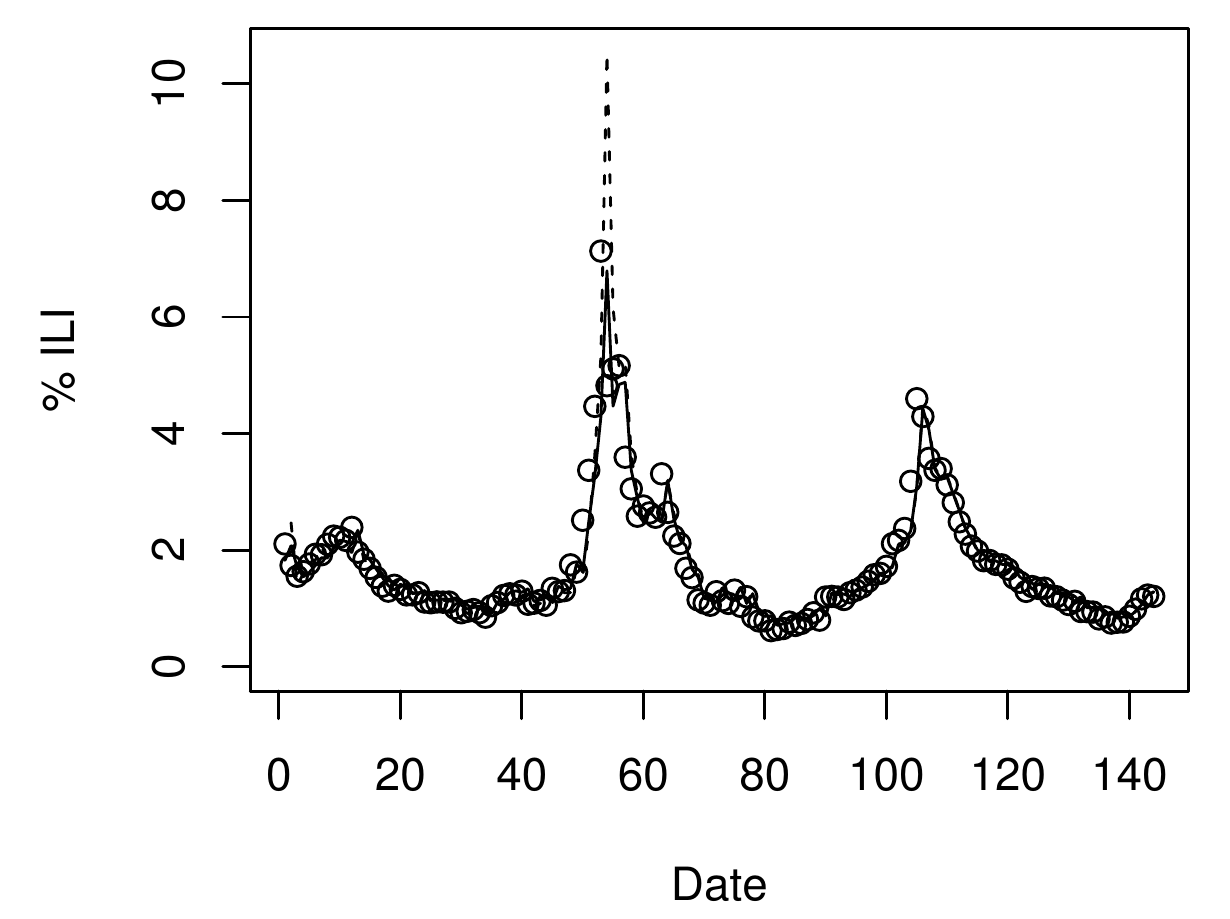
\includegraphics[width=0.9\textwidth,height=0.6\textwidth]{03_cdc_fit_bodnar_thesis.png}
  \caption{Twitter's forecasting (dashed lines) and retroactive measurements (solid lines) compared to the CDC's reported ILI rates (circles) for the whole United States. From \cite{bodnar_data_2015}.}
  \label{fig:cdc_fit_bodnar_thesis}
  \end{figure}
  
Applying the above-described autocorrelation model, Bodnar was able to achieve a very close fit to the official Twitter data (see Figure~\ref{fig:cdc_fit_bodnar_thesis}). In the following chapter, I will describe my attempts to reproduce these findings based on the raw results from the Twitter classifier as well as to repeat the tables and figures shown above based on part of the processed data and code sources provided by Bodnar. 

In Section~\ref{sec:comparison_cdc}, I will focus on results reproducibility by trying to analyse and compare the results from the Twitter classifier with the official flu data from the CDC. In Section~\ref{sec:methods_reproduce}, on the other hand, I will describe my attempts to reproduce two figures and one table from \cite{bodnar_data_2015} by using the processed data and code provided to me, i.e. it contains my efforts to ensure methods reproducibility. Finally, Chapter~\ref{ch:discussion} contains further remarks on the methods and results reproducibility of the findings in \cite{bodnar_data_2015} as well as additional comments regarding inferential reproducibility.

Note that neither Section~\ref{sec:comparison_cdc} nor Section~\ref{sec:methods_reproduce} contain an exhaustive attempt of achieving results and methods reproducibility, respectively. In addition, one might very well argue that true results reproducibility can only be tested by recollecting a Twitter data set of similar size, rewriting the Twitter classifier, and finally comparing the results from the classified tweets to the official CDC data. However, I argue that using the same classified data set used in \cite{bodnar_data_2015} still offers the possibility to test results reproducibility, namely by employing different statistical methods to compare the results from the Twitter classifier to the official CDC data. Mere methods reproducibility, on the other hand, would only focus on recreating the exact findings and figures from \cite{bodnar_data_2015}.

\thispagestyle{empty}
\cleardoublepage

\chapter{(Almost) big data: How to analyse 2.8 billion tweets}
\label{ch:data_set_description}
In this chapter, I will describe the basic characteristics of the data set used by me in this thesis. The largest part of the data aggregation, rectification, and analysis was done using statistical programming language ``R" \citep{rbase_2017}, even though some aggregation and transformation steps were also done using the Python programming language \citep{rossum_1995_python}. In the following, I will cite each library I have used for the data aggregation and analysis. However, since I used several libraries at multiple occasions for my work, I will only cite them when they are mentioned the first time. In order to provide a maximum of reproducibility, all libraries, data sets, custom-written functions, and their output are made avaialable on Github including a detailled description of the exact version of the libraries that were used for the creation of the findings presented in this thesis.

\section{The nature of the data beast}
\label{sec:starting}

At the beginning of my analysis, I was handed a data set with tweet ratings, subdivided into three different sets: 

\begin{itemize}
  \item \texttt{all\_tweets} contains the whole set of rated tweets (2'847'039'672~tweets)
  \item \texttt{one\_hundred} contains the rated tweets of those users who sent at least 100 tweets (42'611'004~tweets)
  \item \texttt{sick\_users} contains the rated tweets of all those users who sent at least one sick tweet (4'131'650~tweets)
\end{itemize}

Each of the sets contains a row per tweet with the following six columns: 

\begin{knitrout}
\definecolor{shadecolor}{rgb}{0.969, 0.969, 0.969}\color{fgcolor}\begin{kframe}
\begin{verbatim}
##          userID longitude latitude       time sick state
## [1,] 1000007198 -86.34844 39.63168 1424580963    0    30
## [2,] 1000007198 -86.34844 39.63168 1424580963    0    30
## [3,] 1000009051 -87.63464 24.39631 1409880397    0    56
## [4,] 1000009051 -87.63464 24.39631 1409880397    0    56
## [5,] 1000010509 -90.14008 29.86666 1394405061    0    36
## [6,] 1000010509 -90.13791 29.88957 1411750890    0    36
\end{verbatim}
\end{kframe}
\end{knitrout}

\begin{itemize}
  \item \texttt{userID} A unique identifier of each Twitter user in the data set
  \item \texttt{longitude} The geographical longitude of the location in which the tweet was sent (in decimal degrees)
  \item \texttt{latitude} The geographical latitude  of the location in which the tweet was sent (in decimal degrees)
  \item \texttt{time} A UNIX timestamp marking the time when tweet was sent
  \item \texttt{sick} A binary variable indicating whether tweet was labelled as ``sick" (=1) or ``healthy" (=0) by the Twitter classifier
  \item \texttt{state} The code for the U.S. state (or District of Columbia) in which the tweet was sent
\end{itemize}

I ignored the \texttt{one\_hundred} data set and only analysed the other two sets. All data sets were handled using the packages ``datatable" \citep{datatable} or ``bigmemory" \citep{bigmemory}.

\section{Description of the \texttt{sick\_users} data set}
\label{sec:sick_user_exploratory}


As mentioned above, the \texttt{sick\_users} data set should contain all tweets from those users who had at least one of their tweets labelled as ``sick" by the classifier.

First, I preprocessed and filtered the data set in order to remove all those tweets that were sent from outside the U.S. mainland (e.g. from the northern Mexico or southern Canada) or were otherwise incorrectly geolocated (e.g. having coordinates which locate the tweeter in the middle of the ocean). To do so, I excluded all tweets lying outside a rough rectangular window with W $-125$° to W $-66$° representing the longitudinal and N $25$° to N $50$° representing the latitudinal expansion of the window. This way, a total of $42'860$ entries were removed with $4'088'790$ entries remaining. As Figure~\ref{fig:hexbincontinent} shows, most of these tweets were clustered around cities, suburban areas and other population-dense regions of the U.S. You can also see that a considerable amount of the collected tweets was not sent from the United States, but from Mexico or Canada.

In the next step, I ran a custom-written function using a polygon lookup based on the coordinates of each tweet to determine the name of the states and to remove all those tweets which could not be assigned to any specific state. Of course, one might wonder why I did not just use the state code already present in the data set to assign each tweet to its respective state. There are two reasons for this: First, I did not have any reference table relating the state codes to the respective state names. Second, the polygon serves as an additional control for the reliability of the data set. If state codes could not clearly be assigned to a specific state, this would mean that the codes could not be used as reference for future analyis. Luckily, this doesn't seem to be the case. Each state code could clearly be assigned to a specific U.S. state with the sole exception of state code ``56", which comprised all those tweets that came to lie on a state or country border, were sent from Mexico or Canada, or were geolocated to the ocean (see Figure~\ref{fig:canexico_and_removed}).

Most of them either came to lie at the coastline or the Canadian-U.S.-border and the Mexican-U.S.-border, respectively. I removed a total of 180'290 tweets that were sent from either Canada or Mexico (see Figure~\ref{fig:canexico_and_removed}). In order to reassign the unassigned tweets from the coastline, I first changed the coordinates of the ``border cases" by 0.1 degrees longitude and latitude towards the center of the U.S. main land (e.g. if a tweet was sent from northeastern Canadian border, I added 0.1 degrees to its longitude and subtracted 0.1 degrees from its latitude before re-running the code). Those tweets that were still unassigned received the same state name as the majority of their neighbours within a 0.1$\times$0.1 degree window. This way, an additional 211'511 tweets were removed, most of them at the coastline or from the ocean (see Figure~\ref{fig:canexico_and_removed}).

After pre-processing, the \texttt{sick\_users} data set was left with 3'696'989 tweets remaining. These tweets were sent by a total of 213'426 users, meaning that on average, each user sent 17.32 tweets. This is in stark contrast to the mean number of tweets reported in \cite{bodnar_data_2015} (175.59 tweets per user over the whole study period). A slight decrease in the mean tweet number should be expected due to the fact that I discarded those tweets outside the designate time or geographical window. However, a tenfold decrease in mean tweet number seems suspect (the time window analysed in \cite{bodnar_data_2015} was March $3^\textit{rd}$ 2011 to March $4^\textit{th}$ 2015, so only sligthly longer than in my case). As can be in Figure~\ref{fig:histogram_ID_tot} a large part of the Twitter users in the \texttt{sick\_users} data set only sent one or two tweets over the whole study period. Furthermore, the maximal number of tweets sent per user over the course of the 208 week time window was 86, a very low number given the fact that there are Twitter users out there who send over a hundred tweets \textit{per day}.\clearpage

\begin{figure}[htbp!]
  \centering
    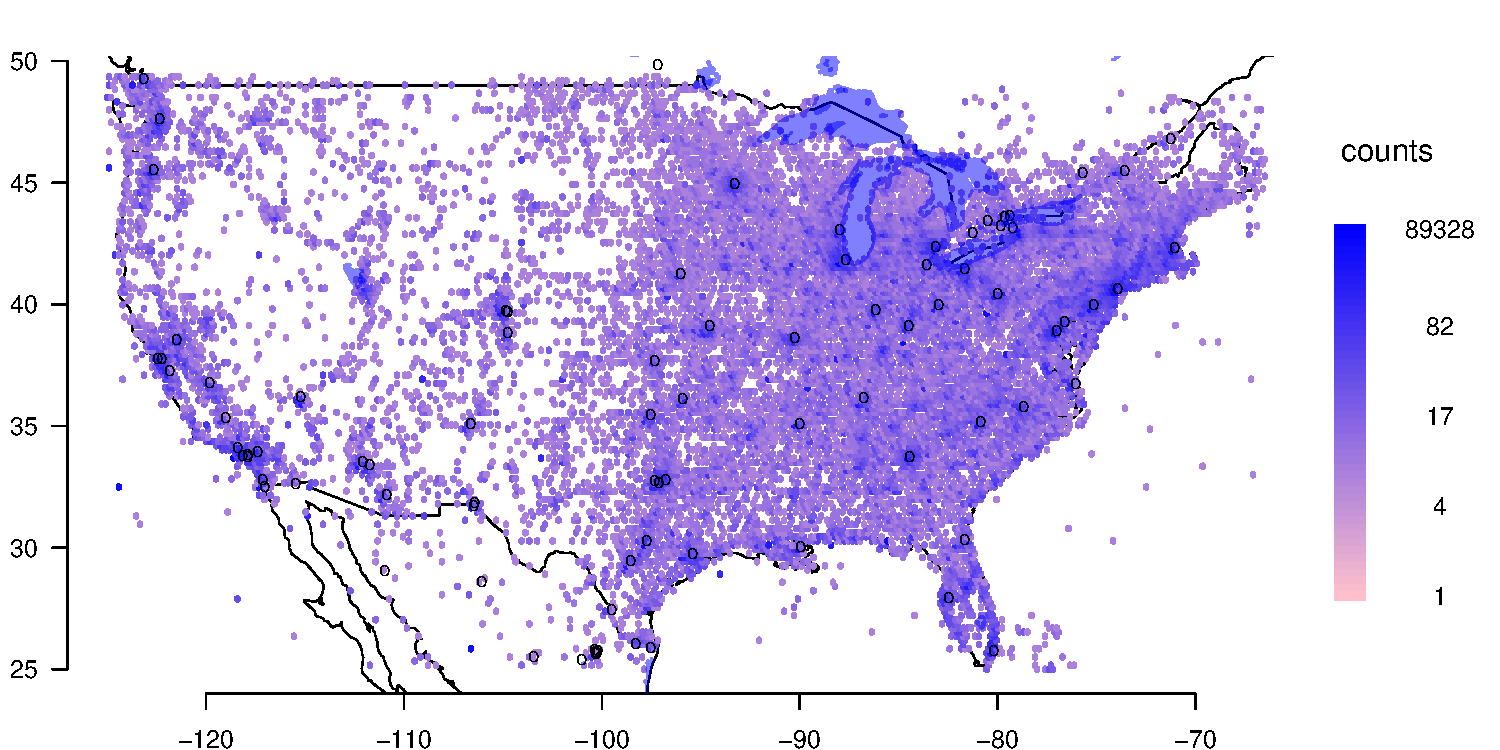
\includegraphics[width=1\textwidth]{4A_HexbinContinent.pdf}
  \caption{Spatial distribution of tweets in the \texttt{sick\_users} data set, aggregated in 12'405 hexagon cells in grid dimensions 148 vertically by 301 horizontally. The black circles correspond to cities with more than 300'000 inhabitants. Note that the colour label does not follow a linear scale. Due to larged difference in the minimal and maximal number of tweets in each bin, I performed a root transformation on the data using the tenth root.}
  \label{fig:hexbincontinent}
  \end{figure}

\begin{figure}[htbp!]
  \centering
    \begin{subfigure}[t]{0.8\textwidth}
    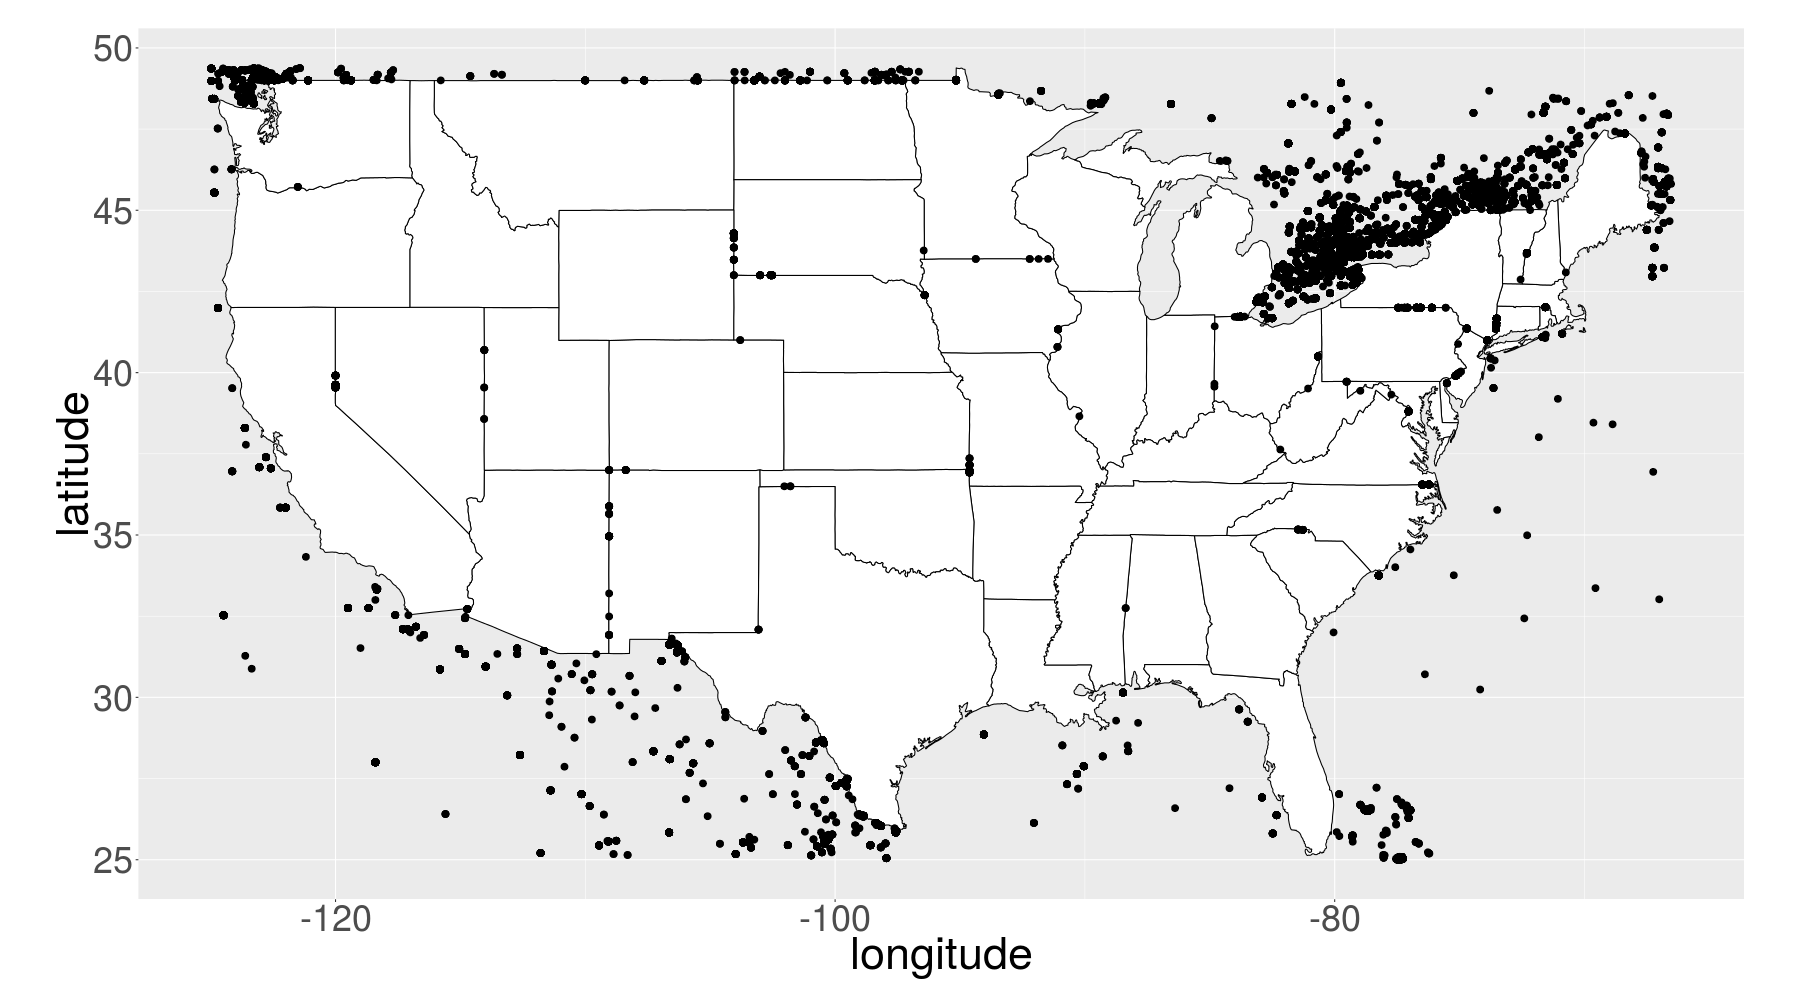
\includegraphics[width=1\linewidth]{04_state56_sick_raw_df.png}
    \caption{}
  \end{subfigure}
  \begin{subfigure}[t]{0.8\textwidth}
  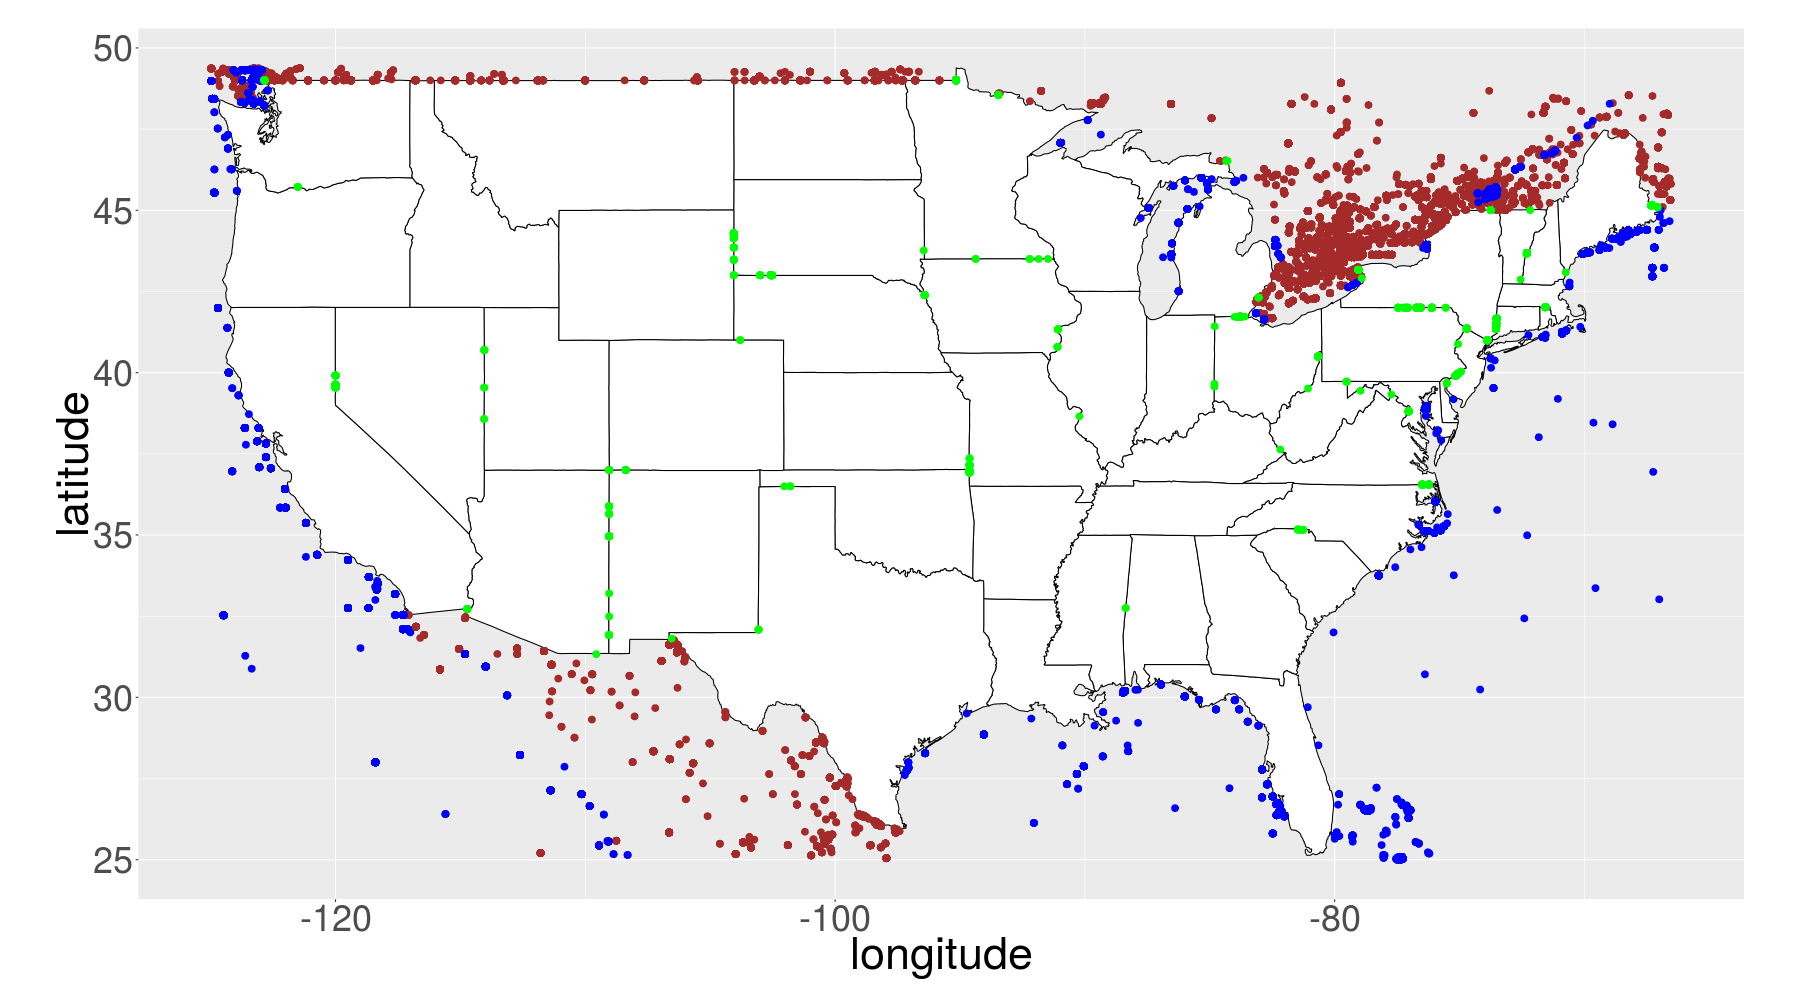
\includegraphics[width=1\linewidth]{05_CanexicoAndRemoved_sick_raw_df.png}
  \caption{}
  \end{subfigure}
  \caption{(a) All tweets in the \texttt{sick\_users} data set whose \texttt{state} variable is coded as ``56", i.e. all tweets that could not be assigned to any specific U.S. state. (b) Tweets whose origins was determined to be in Canada or Mexico (brown) or which could not be assigned to any U.S. state (blue, mainly from the coastline or the ocean) and thus were removed from the \texttt{sick\_users} data set. The green dots represent the tweets that whose \texttt{state} was coded as ``56" as  a code, but which could be recovered by the polygon lookup I performed. Note that the set of tweets shown in (b) is bigger than the set of tweets with state code ``56". This is because some tweets were removed that did \textit{not} have a \texttt{state} code other than ``56", but failed to be assigned to a state by the polygon lookup I performed.}
  \label{fig:canexico_and_removed}
  \end{figure}

\begin{figure}[htbp!]
  \centering
    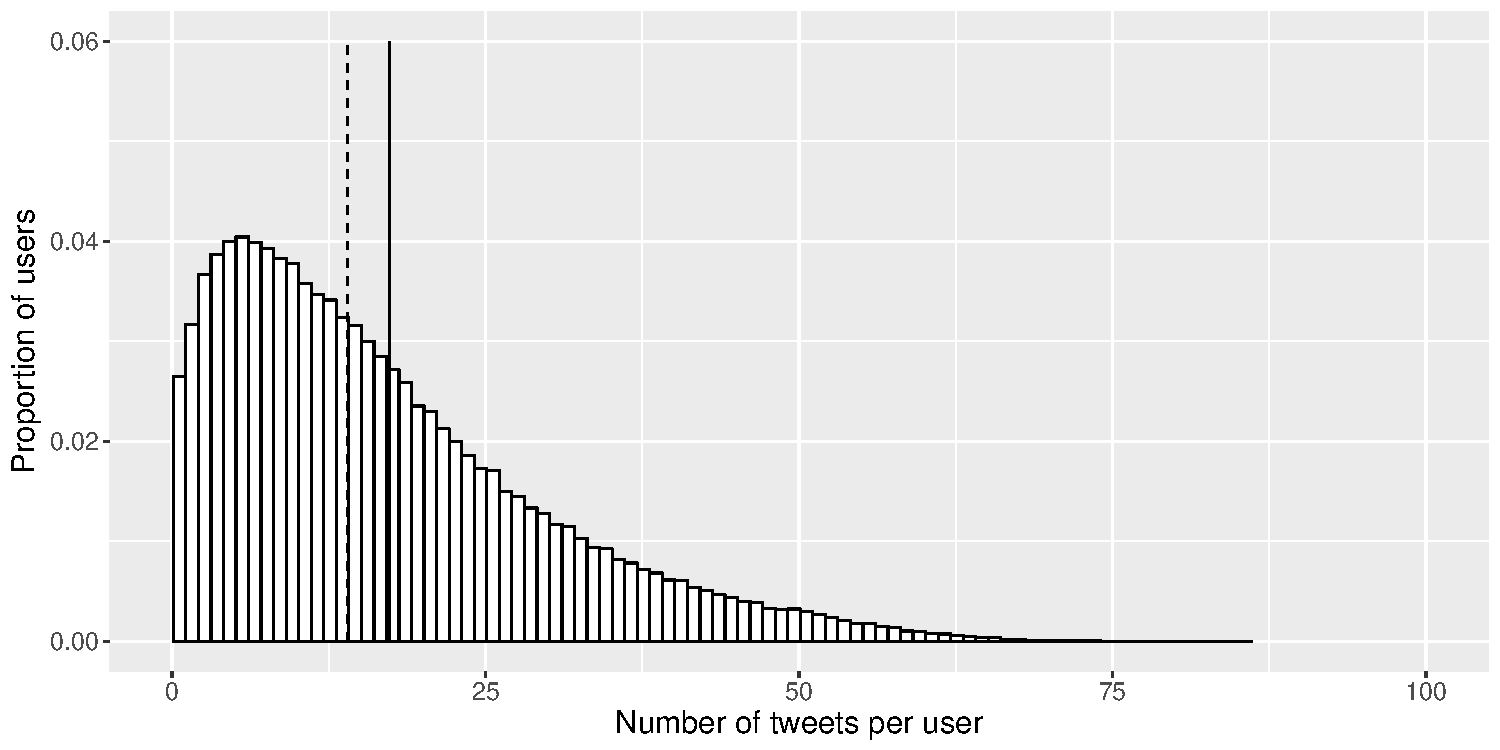
\includegraphics[width=1\textwidth]{06_user_activity_total_sick_raw_df.pdf}
  \caption{Histogram of the number of tweets sent per user in the \texttt{sick\_users} data set during the 208 weeks between 2011-03-05 and 2015-07-11 (bin size = 1 tweet). Mean = 17.32 (solid line); median = 14 (dashed line).}
  \label{fig:histogram_ID_tot}
\end{figure}

\hfill

\begin{figure}[htbp!]
\centering
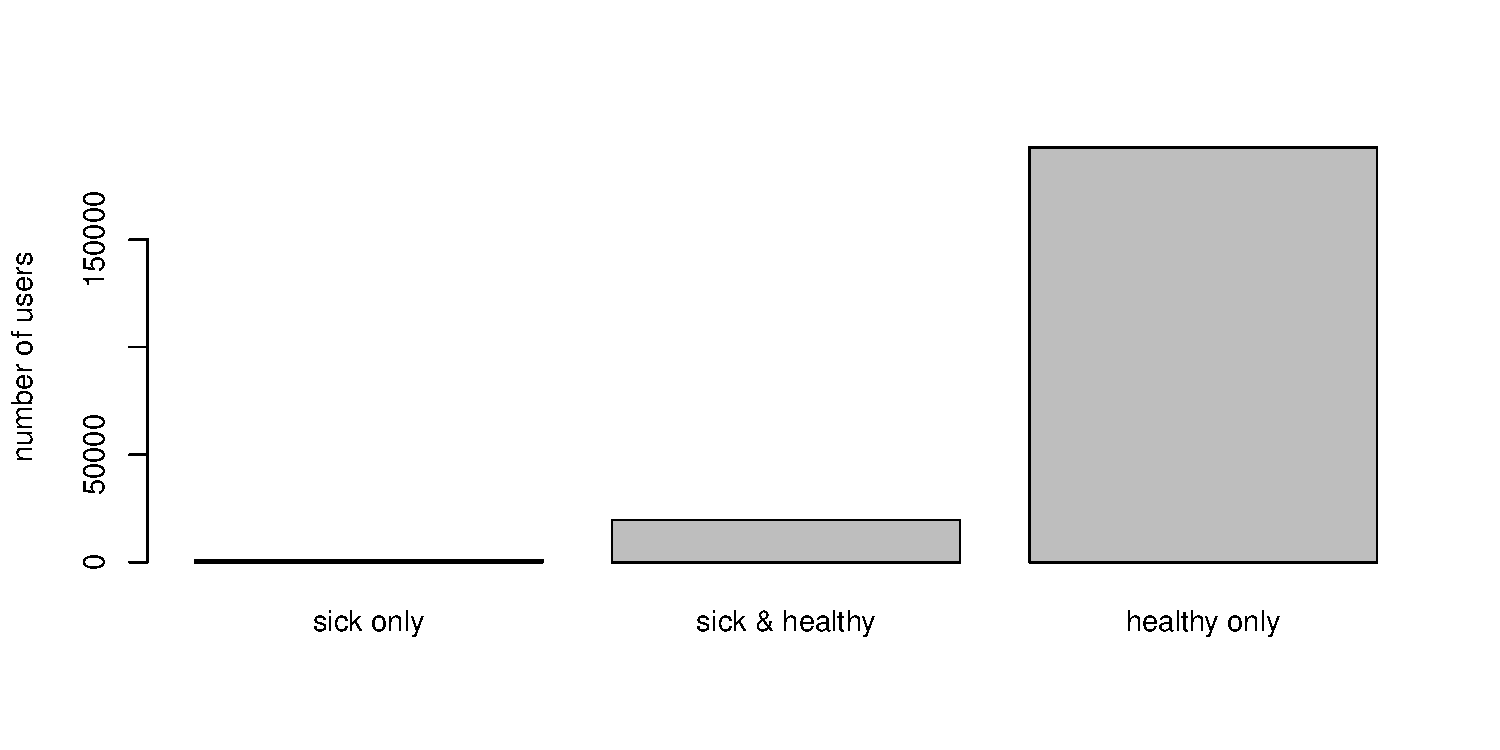
\includegraphics[width=1\linewidth]{07_barplot_sick_raw_df.pdf}
\caption{The total number of users who only sent tweets labelled as ``sick" (919), users who sent at least one tweet labelled as ``sick" and ``healthy" (19'728), and users who only sent tweets labelled as ``healthy" (192'779).}
\label{fig:barplot_sick_df}
\end{figure}

Halfway through 2011, Twitter users sent approximately 200 million tweets per day or 6 billion tweets per month \citep{twitter_million_2011}. If we divide the latter number by the 151 million of Twitter users that were active on a monthly basis by the end of June 30$^\textit{th}$ \citep{twitter_annual_2013}, we get a mean of 39.74 tweets per user per month. Making the conservative assumption that this number remains constant and does not increase, we would expect a mean of 1907.29 tweets per user over the whole four year period between March $3^\textit{rd}$ 2011 to March $4^\textit{th}$ 2015---much more than the 86 tweets sent by the most diligent Twitter user in the \texttt{sick\_users} data set.

One explanation for this discrepancy to the tweet rates found in the \texttt{sick\_users} data set might be found in the fact that the data set only contains geotagged tweets which only represent 0.85 \% \citep{sloan2013knowing} of all tweets. 

If we make the naïve assumption that geotagged tweets represent a subset of all tweets that is uniformly distributed over all Twitter users (in other words: it is assumed that each Twitter user adds geolocation to 0.85\% of his tweets) we receive a mean tweet rate of 2037.9 tweets per user in the \texttt{sick\_users} data set, which is comparable to the mean tweet rate of all Twitter users in the real world (1907.29 tweets per user).

However, \cite{sloan_who_2015} have shown in a recent study that only 58.4 \% of all users have location services enabled and only 3.1\% of all users ever sent a geotagged tweet. Hence, the complete body of geotagged tweets is clustered heavily around a small subset of Twitter users, so that our assumption of the uniform distribution of geotagged tweets over all Twitters users does not hold.

Nevertheless, the information described above allows us to calculate an estimate of the total amount of tweets and users between March $3^\textit{rd}$ 2011 to March $4^\textit{th}$ 2015 using the following formula:
  \begin{align}
\text{tweet rate} = \frac{T_{\text{tot}}}{U_\text{tot}} = \frac{T_{\text{geotagged}} \cdot \frac{1}{0.0085}}{U_\text{geotagged} \cdot \frac{1}{0.031}} \label{eq:3}
  \end{align}

Here, $T_\text{tot}$ and $T_\text{geotagged}$ depict the number of tweets in the real world and the number of tweets in the geotagged subsample, respectively, whereas $U_\text{tot}$ and $U_\text{geotagged}$ denominate the number of Twitter users in the real world and in the geotagged subsample, respectively. 
Applying this formula yields a mean tweet rate of 63.17 tweets per user in the \texttt{sick\_users} data set between March $3^\textit{rd}$ 2011 to March $4^\textit{th}$ 2015, which is higher then the unadjusted tweet rate per user in the \texttt{sick\_users} data set, but still remains considerably lower than the conservative estimate of the real-world tweet rate based on the official Twitter data. Hence, I am led to believe that the \texttt{sick\_users} data set is neither representative of rest of the data set, let alone the total corpus of tweets produced in the real world. This should not come as a suprise, since the \texttt{sick\_users} data set is supposed to contain the tweets of all those users who sent at least one tweet that was classified as ``sick" (Bodnar, personal communication).

However, the large majority of the users within the \texttt{sick\_users} data set never sent a tweet that was labelled as ``sick" by the flu classifier (see Figure~\ref{fig:barplot_sick_df}). In fact, only 20'647 out of 213'426 (or 9.67\%) ever sent such a tweet.

Also, a total of 919 users exclusively sent tweets that were labelled as sick---something that seems rather unlikely to happen. Finally, those 19'728 users who sent both ``sick" and ``healthy" tweets had a significantly lower average tweet rate than those users who only sent ``healthy" tweets (16.01 and 17.53, respectively. $p$ = 0 using a Mann-Whitney U-Test). In fact, a Kolmogorov-Smirnov test indicates that the two subsets do not even follow the same probability distribution ($p$ =0), something that can also easily be observed in Figure~\ref{fig:both_vs_healthy_only_hist}.

Hence, it is unclear how exactly the \texttt{sick\_users} data set was constructed, since it is neither a representative subset of the whole Twitter data set (for that, the percentage for sick tweets is too high, see Section~\ref{sec:full_set}) nor does it exclusively contain tweets from users who had at least one of their tweets labelled as ``sick".

Nevertheless, I used this data set as a basis to develop a basic grasp of the data set as well as to develop functions to analyse the data set in depth and to compare it with official flu data. However, I do not report any more results based on this data set, since the exact selection criteria used for this set are unclear and hence the inferences from it are not to be trusted. All following graphs, calculations and statistics are based on the \texttt{all\_tweets} data set.\clearpage

\begin{figure}[htbp!]
\centering
  \begin{subfigure}[b]{1\textwidth}
  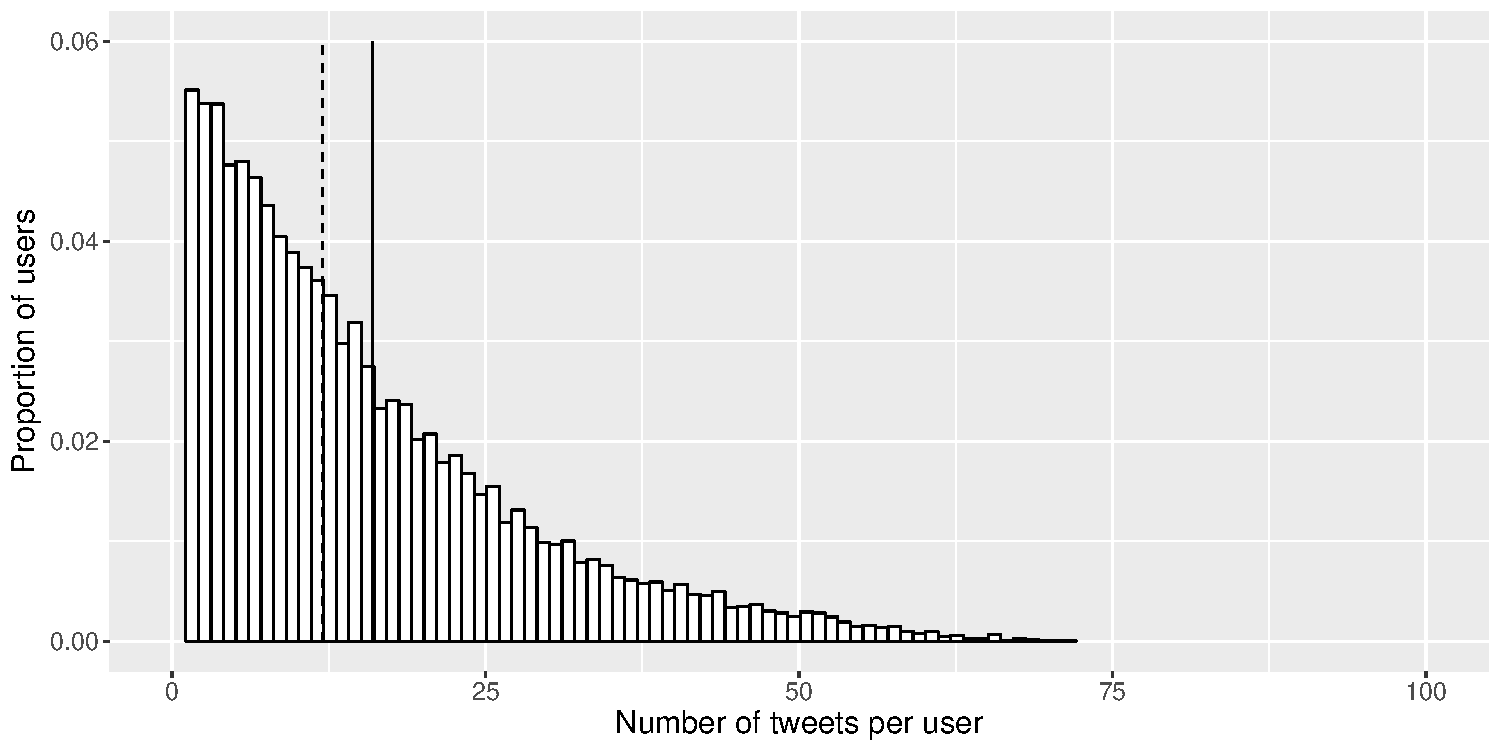
\includegraphics[width=1\linewidth]{08_user_activity_both_sick_raw_df.pdf}
  \caption{}
  \end{subfigure}
  \begin{subfigure}[b]{1\textwidth}
  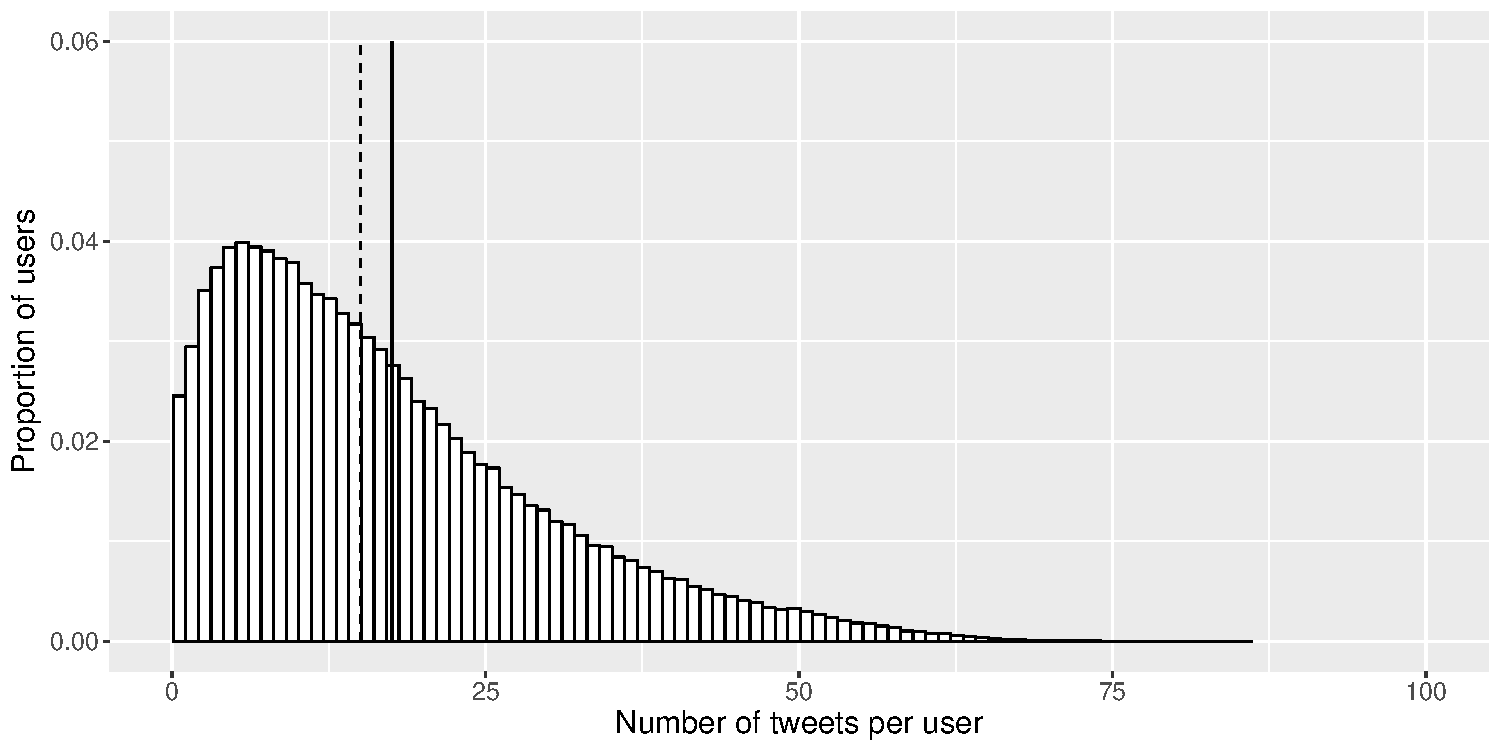
\includegraphics[width=1\linewidth]{09_user_activity_only_healthy_sick_raw_df.pdf}
  \caption{}
  \end{subfigure}
  \caption{Histograms of the number of tweets sent per user during the 208 weeks between 2011-03-05 and 2015-07-11 (bin size = 1 tweet). (a) Users who sent at least one tweet labelled as ``sick" and one tweet labelled as ``healthy".  Mean = 16.01 (solid line); median = 12 (dashed line). (b) Users who never sent a tweet that was labelled as ``sick" by the classifier.  Mean = 17.53 (solid line); median = 15 (dashed line). Mode, median, and mean of the number of tweets sent per user are significantly lower in (a) than in (b). Also, note that by construction (a) does not contain any user who only sent one tweet since the users in this group are defined by having sent at last one tweet labelled ``sick" and one tweet labelled as ``healthy".}
  \label{fig:both_vs_healthy_only_hist}

\end{figure}

\section{Description of the \texttt{all\_tweets} data set}
\label{sec:full_set}

The complete data set consisted of a total of 2'847'039'672 tweets sent by 16'015'981. Hence, it contained more tweets sent by fewer users than the data set reported by \cite{bodnar_data_2015} which consisted of 2'732'174'105 tweets sent by 15'560'328 users. The difference in the number of tweets might simply stem from the fact that the tweets in my data set were collected until July 2015, while the tweets analysed in \cite{bodnar_data_2015} were only collected up to March 2015. However, the stark reduction in the number of users is puzzling and hints at the possibility that I was working with a different data set (also see Section~\ref{sec:diff_data_set} for further discussion). An overview over all differences between the two data sets as well over key statistical indicators of the \texttt{all\_users} data set is given in Table~\ref{tab:data_set_diff}.

\begin{table}[htbp!]
\centering
\caption{Key differences between the data sets reported in \cite{bodnar_data_2015} and the one I analysed. Values in white and grey-coloured rows are based on the raw and pruned data set, respectively.}
\begin{tabular}{l l l l l}
 & Bodnar  & Grüninger & \\ \hline
\# of users  & 15'560'328 & 16'015'981 & raw data set  \\
\cellcolor{grey}\# of users, pruned & \cellcolor{grey}-- & \cellcolor{grey}15'229'049 & \cellcolor{grey}pruned data set\\
\# of tweets  & 2'732'174'105 & 2'847'039'672 & raw data set  \\ 
\cellcolor{grey}\# of tweets  & \cellcolor{grey}-- & \cellcolor{grey}2'764'210'962 & \cellcolor{grey}pruned data set \\
\cellcolor{grey}\# of sick users, 2011--2015 & \cellcolor{grey}182'801 & \cellcolor{grey}27'052 & \cellcolor{grey}pruned data set  \\
\cellcolor{grey}\# of users, 2011 & \cellcolor{grey}45'086 & \cellcolor{grey}175'382 & \cellcolor{grey}pruned data set\\
mean tweet rate, 2011--2015 & 175.59 & 177.76 & raw data set\\
\cellcolor{grey}mean tweet rate, 2011--2015 & \cellcolor{grey}-- & \cellcolor{grey}181.51 & \cellcolor{grey}pruned data set \\
\cellcolor{grey}mean tweet rate, weekly & \cellcolor{grey}-- & \cellcolor{grey}31.42 & \cellcolor{grey}pruned data set\\
median tweet rate, 2011--2015 & 10 & 9 & raw data set\\
\cellcolor{grey}median tweet rate, 2011--2015 & \cellcolor{grey}-- & \cellcolor{grey}9 & \cellcolor{grey}pruned data set\\
\cellcolor{grey}median tweet rate, weekly & \cellcolor{grey}-- & \cellcolor{grey}32.53 & \cellcolor{grey}pruned data set\\
max. \# of tweets per user, 2011--2015 &  1'119'384 & 1'413'568 & raw data set\\
\cellcolor{grey}max. \# of tweets per user, 2011--2015 & \cellcolor{grey}-- & \cellcolor{grey}1'413'568 & \cellcolor{grey}pruned data set\\
min. \# of tweets per user, 2011--2015 & 1 & 1 & raw data set\\
\cellcolor{grey}min. \# of tweets per user, 2011--2015 & \cellcolor{grey}-- & \cellcolor{grey}1 & \cellcolor{grey}pruned data set\\
\end{tabular}
\end{table}

In a first step, I removed all tweets before 2011-03-05 and after 2015-07-11 as well as outside the rough geographical window around the U.S. mainland (W $-125$°, W $-66$°, N $25$° , N $50$° ) as described above, and aggregated the remaining 2'764'210'962 tweets and 15'229'049 users with regard to states and weeks in which the tweets where sent, i.e. I calculated the number of tweets sent within a given week in a given state.

The cut-off date for each week corresponded to the dates the official CDC flu reports were published. All tweets within the seven day time window leading up to a specific data were assigned to said date, including the tweets sent on that date. For example, if a tweet was sent on 2015-07-11, 2015-07-07 or 2015-07-05 it was assigned to 2015-07-11. However, if it was sent on 2015-07-04 it was assigned to the previous week ending on 2015-07-10.

Since there are a total of 208 weeks between 2011-03-05 and 2015-07-11 and a total of 50 different state labels in the original data set (48 labels for states on the U.S. mainland, 1 label for the District of Columbia and 1 label for the tweets that could not be assigned to any of the other 49 areas), I received a data set with 10'400 rows after aggregation (one for each state-week-pair). Each row has the following six columns:

\begin{knitrout}
\definecolor{shadecolor}{rgb}{0.969, 0.969, 0.969}\color{fgcolor}\begin{kframe}
\begin{verbatim}
##    week state sick  total healthy     sick_per
## 1:   23    34    1  86616   86615 1.154521e-05
## 2:  194    43    2  69629   69627 2.872366e-05
## 3:  155    16    0 140482  140482 0.000000e+00
## 4:   67    24  686 181757  181071 3.774270e-03
## 5:   40    28    0 101685  101685 0.000000e+00
## 6:   17     0    0  10142   10142 0.000000e+00
\end{verbatim}
\end{kframe}
\end{knitrout}

\begin{itemize}
  \item \texttt{week} The week in which the aggregated tweets were sent
  \item \texttt{state} The state in which the tweet were sent
  \item \texttt{sick} The total number of tweets that were labelled as ``sick" in the given week and state
  \item \texttt{total} The total number of tweets sent in the given week and state
  \item \texttt{healthy} The total number of tweets that were not labelled as ``sick" in the given week and state
  \item \texttt{sick\_per} The percentage of tweets labelled as sick among the total tweets sent in the given week and state
\end{itemize}

Next, I added the corresponding date and state name to each week and state index, respectively. In order to assign state names to their respective state labels, I used the label/name relationships established in the \texttt{sick\_users} data set (see section~\ref{sec:sick_user_exploratory}). Since tweets with state code ``56" predominantly stemmed from the Mexico and Canada or other areas outside the U.S. mainland (see Figure~\ref{fig:canexico_and_removed}), I removed all corresponding state/week pairs from the aggregated data set (223'352'319 tweets in total), resulting in a data set with 10'192 rows and 16 columns (see below), containing a total of 2'614'711'121 tweets from 15'229'049 users aggregated over states and weeks.

\begin{knitrout}
\definecolor{shadecolor}{rgb}{0.969, 0.969, 0.969}\color{fgcolor}\begin{kframe}
\begin{verbatim}
##    week state sick  total healthy     sick_per            statename       date
## 1:   23    34    1  86616   86615 1.154521e-05            wisconsin 2011-08-13
## 2:  194    43    2  69629   69627 2.872366e-05             nebraska 2014-11-22
## 3:  155    16    0 140482  140482 0.000000e+00             delaware 2014-02-22
## 4:   67    24  686 181757  181071 3.774270e-03             kentucky 2012-06-16
## 5:   40    28    0 101685  101685 0.000000e+00            tennessee 2011-12-10
## 6:   17     0    0  10142   10142 0.000000e+00 district of columbia 2011-07-02
\end{verbatim}
\end{kframe}
\end{knitrout}

There were a total amount of 1'189'809 tweets labelled as ``sick", a number that is considerably larger than the 20'894 tweets labelled as ``sick" in the \texttt{sick\_users} data set. This further shows that the latter does not contain the full subset of tweets labelled as ``sick". Relatively speaking, 0.05~\% of all tweets in the \texttt{all\_tweets} data set were labelled as ``sick" (as opposed to 9.67~\% in the \texttt{sick\_users} data set).

The total amount of users who have sent at least one tweet labelled as sick during the study period was 27'052. Note that this is an upper estimate, since a user could be classified as ``sick" more than once between 2011-03-05 and 2015-07-11. Since my analysis rests on weekly aggregated data, I was not be able to differentiate between a user who is classified as sick two times and two individual users who are classified as sick once. However, this is only a problem when assessing the total number of tweeters over the whole study period---it does not pose an obstacle when looking at the data categorised by weeks and/or states or at averaged data.

What is peculiar, however, is the fact that the total number of sick users found in the Twitter data set over the whole study period is considerably lower than the number reported in \cite{bodnar_data_2015} (27'052 vs. 182'801 users, respectively), despite the former being an upper estimate of the total number of individual sick users. On the other hand, the number of individual users found in the data set during the first year (2011) for the whole country is larger than the one reported by \cite{bodnar_data_2015}: 175'382 and 45'086, respectively.

Using the information that only 3.1~\% of all users send geotagged tweets \citep{sloan2013knowing}, we can estimate the total number of Twitter users that were active in 2011 based on the two mentioned sample estimates, respectively. While the former sample estimate gives us an estimated average of 5'657'476 active users in 2011, the latter estimate based on \cite{bodnar_data_2015} only amounts to 1'454'387 total active users in 2011. Both numbers are a far cry from the roughly 19 (March 2011) to 30 (December 2011) million of monthly active Twitter users officially reported by Twitter in 2011 \citep{twitter_annual_2013}, even though part of this discrepancy might be explained by the first two months of 2011 are missing from the collection of the Twitter data sets Bodnar and I were working on.These points give additional reason to believe that the data reported in \cite{bodnar_data_2015} are not the same as the data I analysed for this thesis.

In addition, I could observe a very peculiar difference in the mean tweet frequency between healthy and sick users. While healthy users had an unadjusted mean tweet rate of 31.42 tweets per week, sick users had an unadjusted mean tweet rate of 45.95 tweets per week (see Figure~\ref{fig:avg_tw_diff}), a difference that is highly significant (Mann--Whitney U-Test, $p$ =0). 

Also, the unadjusted mean tweet rate per week of all users combined (31.42) is six times smaller than the mean tweet rate over the whole study period (181.51). The same holds true for the unadjusted median tweet rate (32.53 tweets per user per week vs. 9 tweets per user over the whole study period). These differences make intuitive sence, since

Finally, by applying Equation~\ref{eq:3} described in Section~\ref{sec:sick_user_exploratory}, we can estimate the adjusted mean (114.6 tweets per user) and median (118.64 tweets per user) of the Twitter rate of the whole Twitter population in 2011, as well the mean tweet rate for sick (167.6 tweets per user) and healthy (114.58 tweets per user) subpopulation, respectively.\clearpage

\begin{figure}[htbp!]
\centering
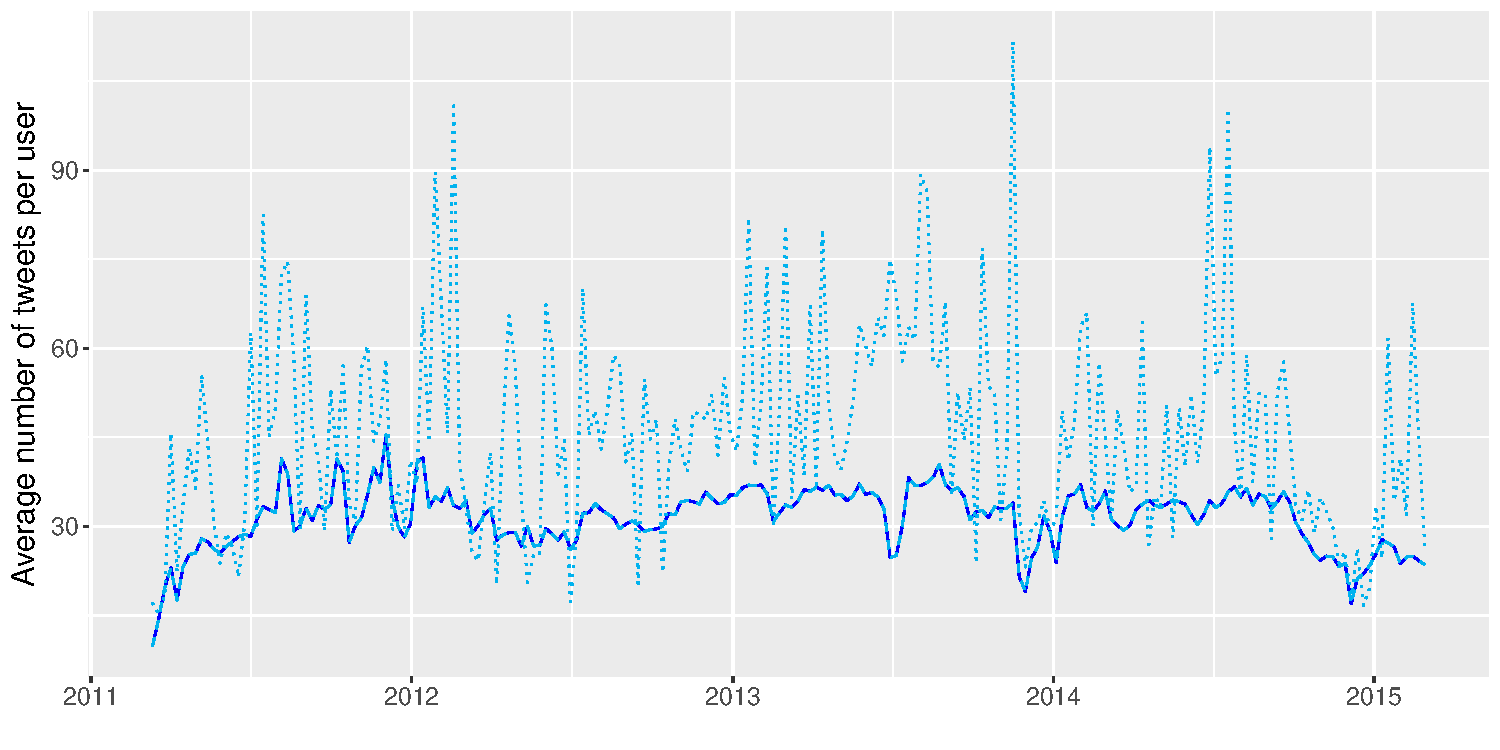
\includegraphics[width=1\linewidth]{10_avg_tw_sick_healthy.pdf}
\caption{The unadjusted mean number of tweets per week sent by sick users (dotted light blue), healthy user (dashed light blue), and total users (solid blue), respectively.}
\label{fig:avg_tw_diff}
\end{figure}

\thispagestyle{empty}
\cleardoublepage

\chapter{What does the classified Twitter data set reveal about the flu?}
\label{ch:results}

In the first part of this chapter, I will describe the performance of the flu classifier compared to the weekly influenza rate estimates of the CDC (Section~\ref{sec:comparison_cdc}. In addition to this, I will critically assess the Twitter classifiers ability to predict the CDC's ILI reports as described in \cite{bodnar_data_2015}, in order to test which of the described findings are reproducible.

In the second part of this chapter, I will present my attempts to faithfully reproduce two key figures and one table from \cite{bodnar_data_2015} by using the processed data and the code provided to me. This part will therefore shed light on the question whether the methodological and theoretical descriptions provided in \cite{bodnar_data_2015} as well as the available data and code basis are sufficient to ensure methods reproducibility.

\section{Can the Twitter classifier compete for gold?}
\label{sec:comparison_cdc}

The CDC publishes weekly ILI reports containing the number of patients with ILI symptoms relative to the total number of patients in the more than 2'800 outpatient healthcare providers that are part of the U.S. Outpatient Influenza-like Illness Surveillance Network (ILINet). The reports provided by the ILINet are commonly regarded as the gold standard of epidemiological flu data, so comparing the performance of the flu classifier is an important first step to assess its validity. 

However, since correctly diagnosing the flu can only be done through microbiological analysis, the CDC uses ``influenza-like illnesses (ILI)" as a proxy to assess the prevalence of influenza cases in the United States. ILI are defined as ``fever (temperature of 100°F [37.8°C] or greater) and a cough and/or a sore throat without a known cause other than influenza" \citep{cdc_surveillance_2016}. It is therefore important to note that I am not comparing the Twitter classifier's results to the number of flu cases in the U.S., but only to the number of registered ILI cases, i.e. a proxy of flu prevalence. But since the CDC's data are commonly very reliable and since the Twitter classifier itself uses the content of single tweets as a proxy between sick and healthy users, these kinds of comparisons make sense. 

Before doing so, however, I will provide additional descriptive statistics of the data set.

\subsection{Spatio-temporal patterns of Twitter usage}

Figure~\ref{fig:tweets_seasonal_full} shows the total number of tweets sent per week relative to the total number of tweets sent in the study period. No obvious pattern is discernible other than an increase in weekly tweets until the third quarter of 2014 when a sudden dip in tweet activity occurs. The activity pattern of the tweets labelled as ``healthy" is almost indiscernible from the temporal pattern of the complete data set. When looking at the weekly amount of tweets labelled as ``sick" one can see a different pattern: The weekly activity is fluctuating more strongly and shows clearly discernible peaks towards the end and the beginning of each year. This pattern turns out to be even more pronounced when correcting for the total amount of tweets sent per week. 

A Kolmogorov-Smirnov test reveals that the weekly activity of the tweets labelled as ``sick" is in fact significantly different from the weekly activity of the tweets labelled as ``healthy" ($p$ = 0.0264 and $p$ = 0 for the normalised and not normalised weekly tweet counts, respectively). As can be seen in Figure~\ref{fig:tweets_seasonal_healthy_sick} the tweets labelled as ``sick" follow a markedly different temporal pattern than those labelled as ``healthy". Also, the distribution of the latter is virtually indistinguishable from the distribution of the total amount of tweets.

Repeating the calculations describe above using number of Twitter users instead of number of tweets yields similar results (see Figure~\ref{fig:tweets_seasonal_healthy_sick_user}; $p$ = 0 and $p$ = 0 for the normalised and not normalised weekly user activity, respectively), However, using Twitter users instead of single tweets as basis for the aggregation reduces the weekly fluctuations of the weekly ``sick" rates considerably (see Section~\ref{sec:comp_cdc} for further discussion.)

Next, I looked at the total amount of tweets sent in each state. As can be seen in Figures~\ref{fig:tweets_state_full}, \ref{fig:tweets_state_full_scatter}, and \ref{fig:tweets_state_full_scatter_log} the relative distribution per state largely follows the relative distribution of the state population. Notable exceptions are Maryland, New Jersey, West Virginia, and Delaware, which were the origin of many more tweets than expected, as well as New York, Idaho, Montana, District of Columbia, Wyoming, and Vermont, from where considerably fewer tweets originated than would be expected with regard to its population.

When comparing the relative number of tweets labelled as ``healthy" with those labelled as ``sick", we can see slight differences in the distribution, which become even more accentuated when normalising with the total number of tweets per state (Figure~\ref{fig:tweets_state_healthy_sick}). However, the states with the most pronounced differences (District of Columbia, Montana, South Dakotam, North Carolina) are almost all states or districts, respectively, with a very low overall tweet count (North Carolina being the exception). A Chi-squared test for independence between the two distributions gives a $p$-value of 0.0801. 

Repeating the calculations described above using the number of Twitter users instead of the number of tweets yields similar results (Figures~\ref{fig:tweets_state_full_user}, \ref{fig:tweets_state_full_scatter_user}, \ref{fig:tweets_state_full_scatter_user_log}, and \ref{fig:tweets_state_healthy_sick_user}; $p$ = 0.0823).\clearpage

\begin{figure}[htbp!]
\centering
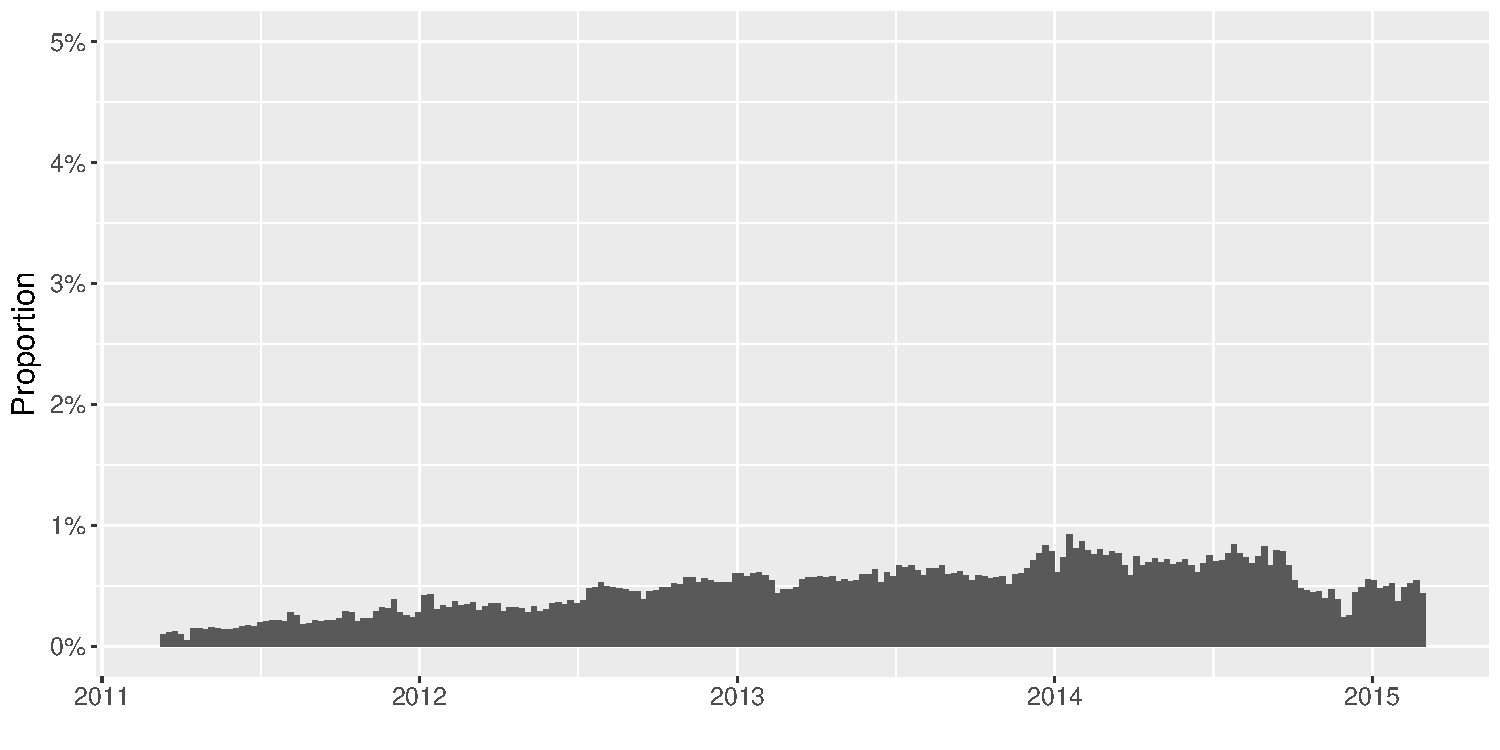
\includegraphics[width=1\linewidth]{11_activity_total_date_Twitter_full_aggregated.pdf}
\caption{Relative number of tweets sent per week in the \texttt{all\_tweets} data set between 2011-03-05 and 2015-07-11 (bin size = 1 week).}
\label{fig:tweets_seasonal_full}
\end{figure}

\begin{figure}[htbp!]
\centering
  \begin{subfigure}[t]{1\textwidth}
  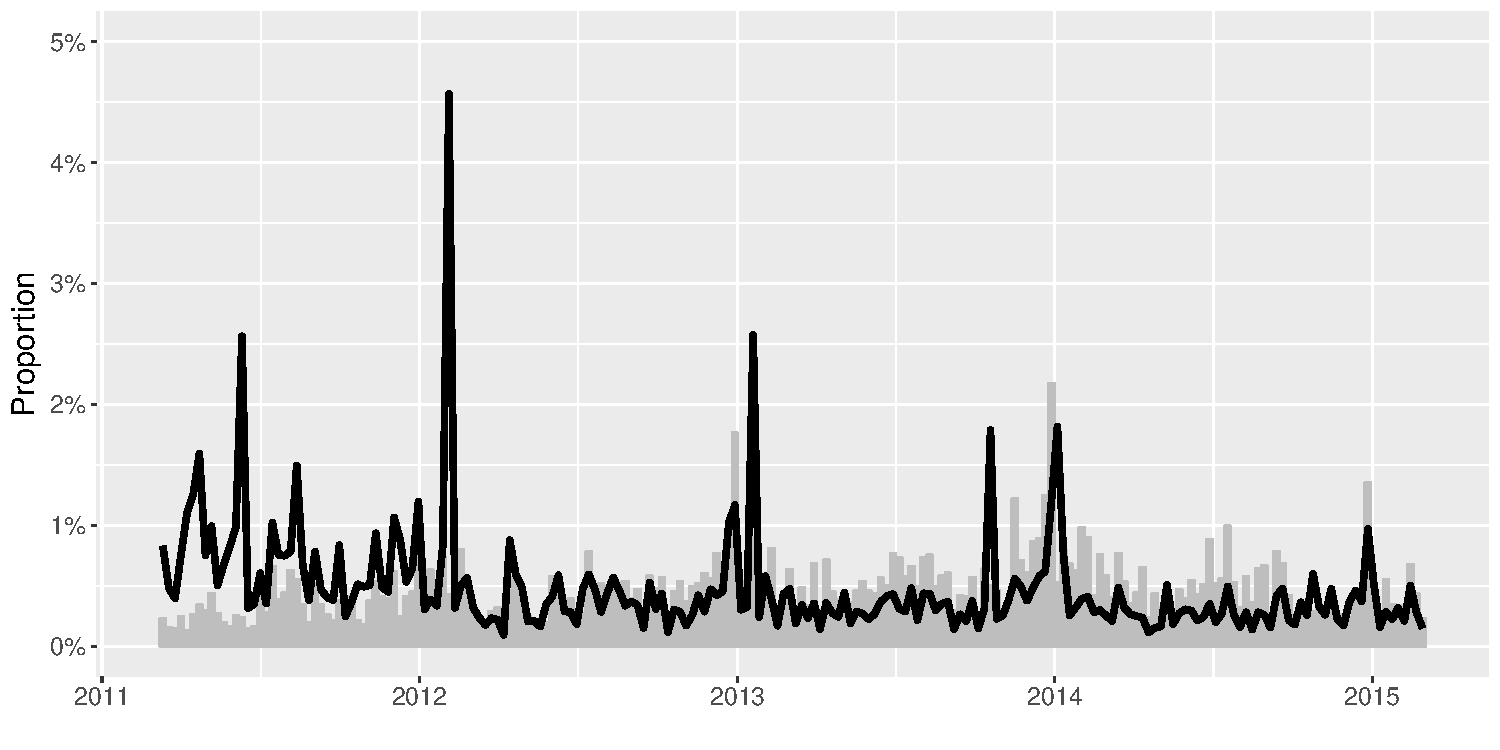
\includegraphics[width=1\linewidth]{12_activity_sick_date_Twitter_full_aggregatedoverlay.pdf}
  \caption{}
  \end{subfigure}
  
  \bigskip 

    \begin{subfigure}[t]{1\textwidth}
  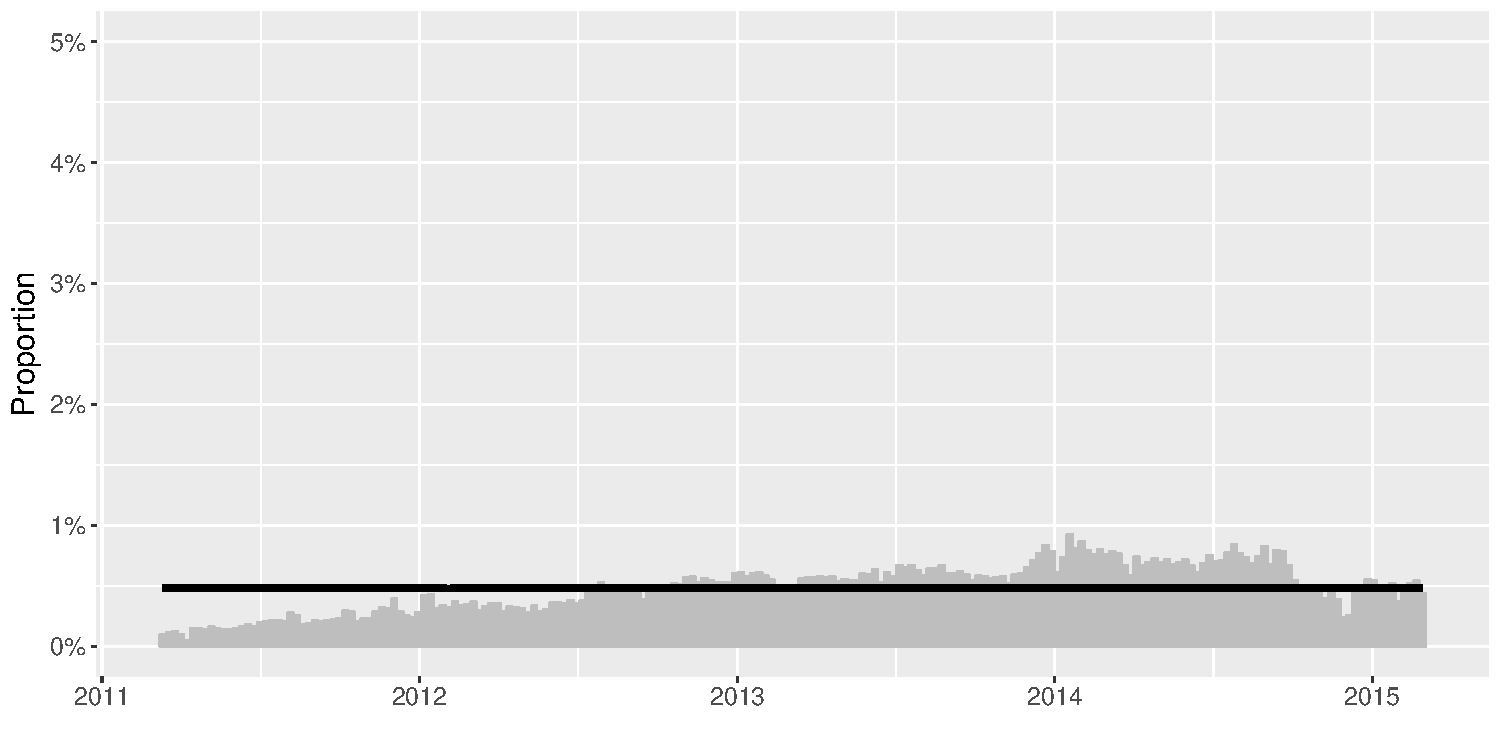
\includegraphics[width=1\linewidth]{13_activity_healthy_date_Twitter_full_aggregatedoverlay.pdf}
  \caption{}
  \end{subfigure}
  \caption{Histograms of numbers of the tweets sent per week during the 208 weeks between 2011-03-05 and 2015-07-11 (bin size = 1 week). (a) shows only tweets labelled as ``sick"; (b) shows only tweets labelled as ``healthy" by the classifier. The grey bars indicate the relative number of sick or healthy tweets sent per week without normalisation. The black lines indicate the relative number of sick or healthy tweets sent per week normalised by the total amount of tweets sent in that week.}
  \label{fig:tweets_seasonal_healthy_sick}
\end{figure}

\begin{figure}[htbp!]
\centering
  \begin{subfigure}[t]{1\textwidth}
  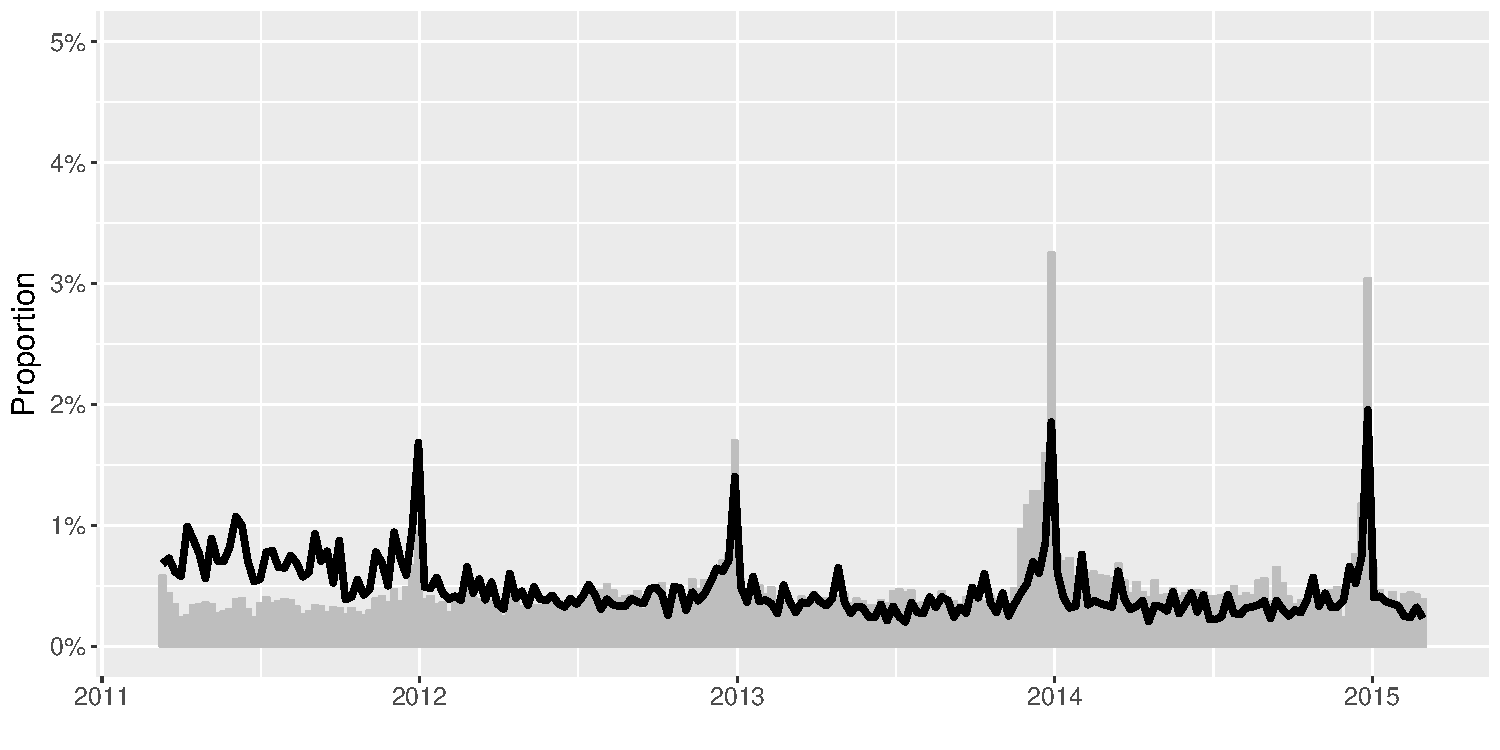
\includegraphics[width=1\linewidth]{12B_activity_sick_user_date_Twitter_full_aggregatedoverlay.pdf}
  \caption{}
  \end{subfigure}
  
  \bigskip 

    \begin{subfigure}[t]{1\textwidth}
  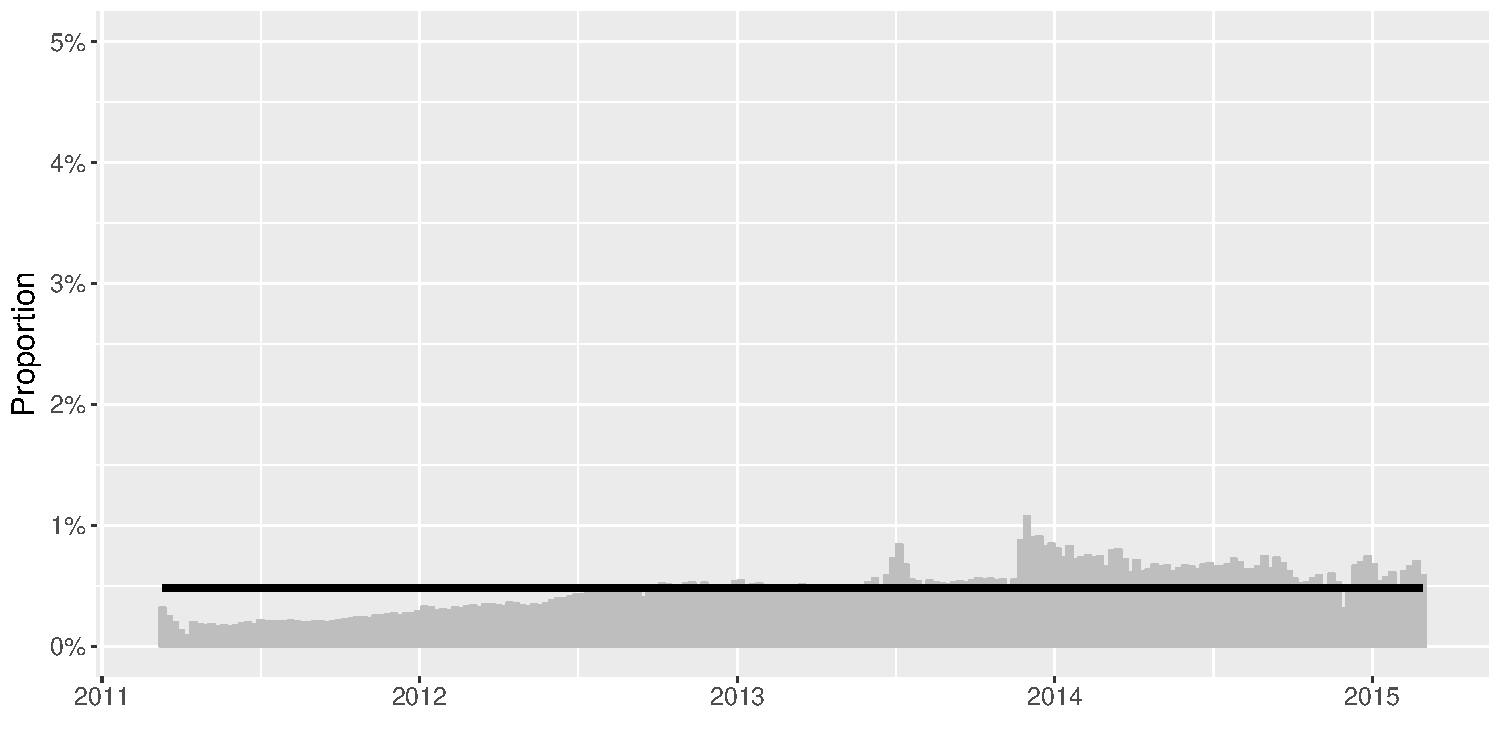
\includegraphics[width=1\linewidth]{13B_activity_healthy_user_date_Twitter_full_aggregatedoverlay.pdf}
  \caption{}
  \end{subfigure}
  \caption{Histograms of numbers of the tweets sent per week during the 208 weeks between 2011-03-05 and 2015-07-11 (bin size = 1 week). (a) shows only tweets labelled as ``sick"; (b) shows only tweets labelled as ``healthy" by the classifier. The grey bars indicate the relative number of sick or healthy tweets sent per week without normalisation. The black lines indicate the relative number of sick or healthy tweets sent per week normalised by the total amount of tweets sent in that week.}
  \label{fig:tweets_seasonal_healthy_sick_user}
\end{figure}

\begin{figure}[htbp!]
\centering
\begin{subfigure}[t]{1\textwidth}
  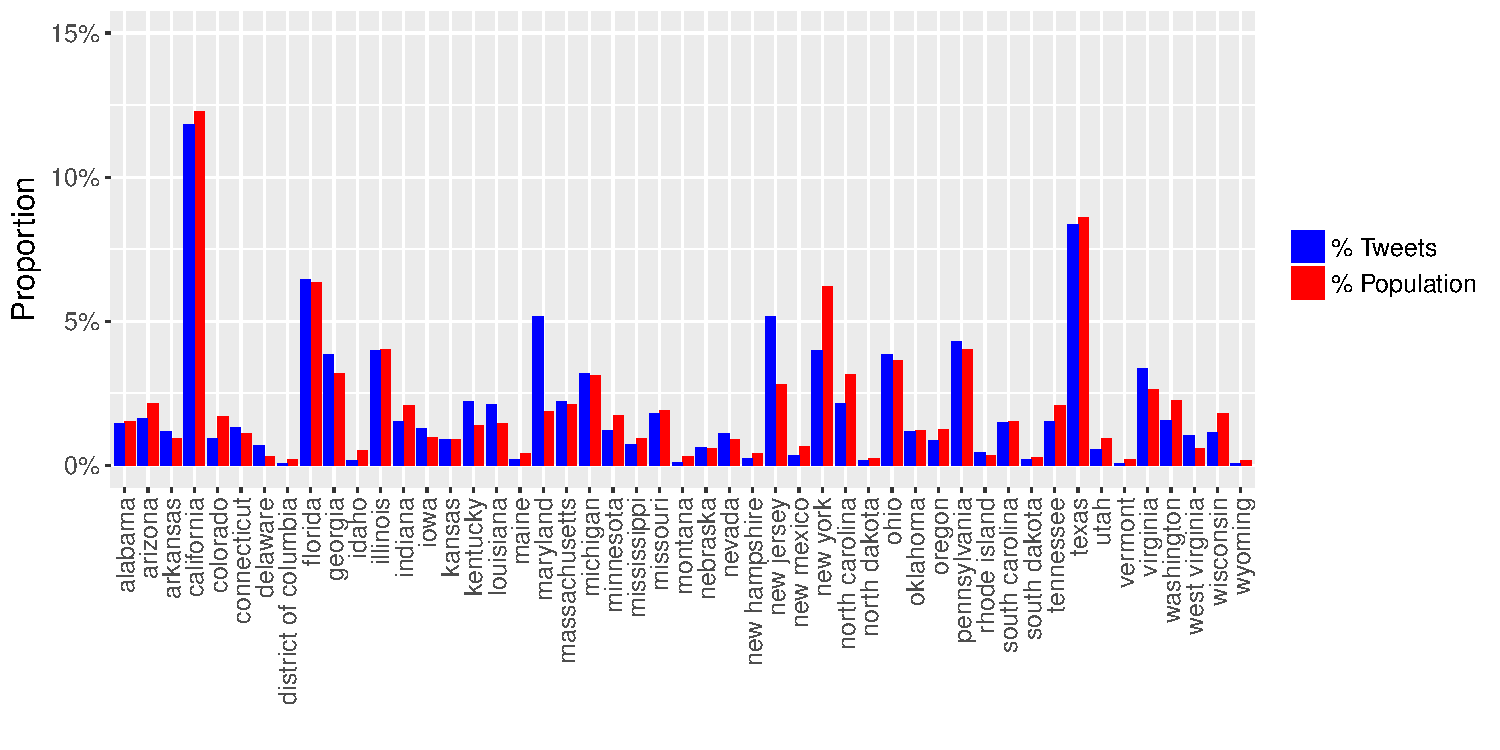
\includegraphics[width=1\linewidth]{14_activity_total_state_Twitter_full_aggregated.pdf}
  \caption{}
  \label{fig:tweets_state_full}
  \end{subfigure}
  
  \begin{subfigure}[t]{1\textwidth}
  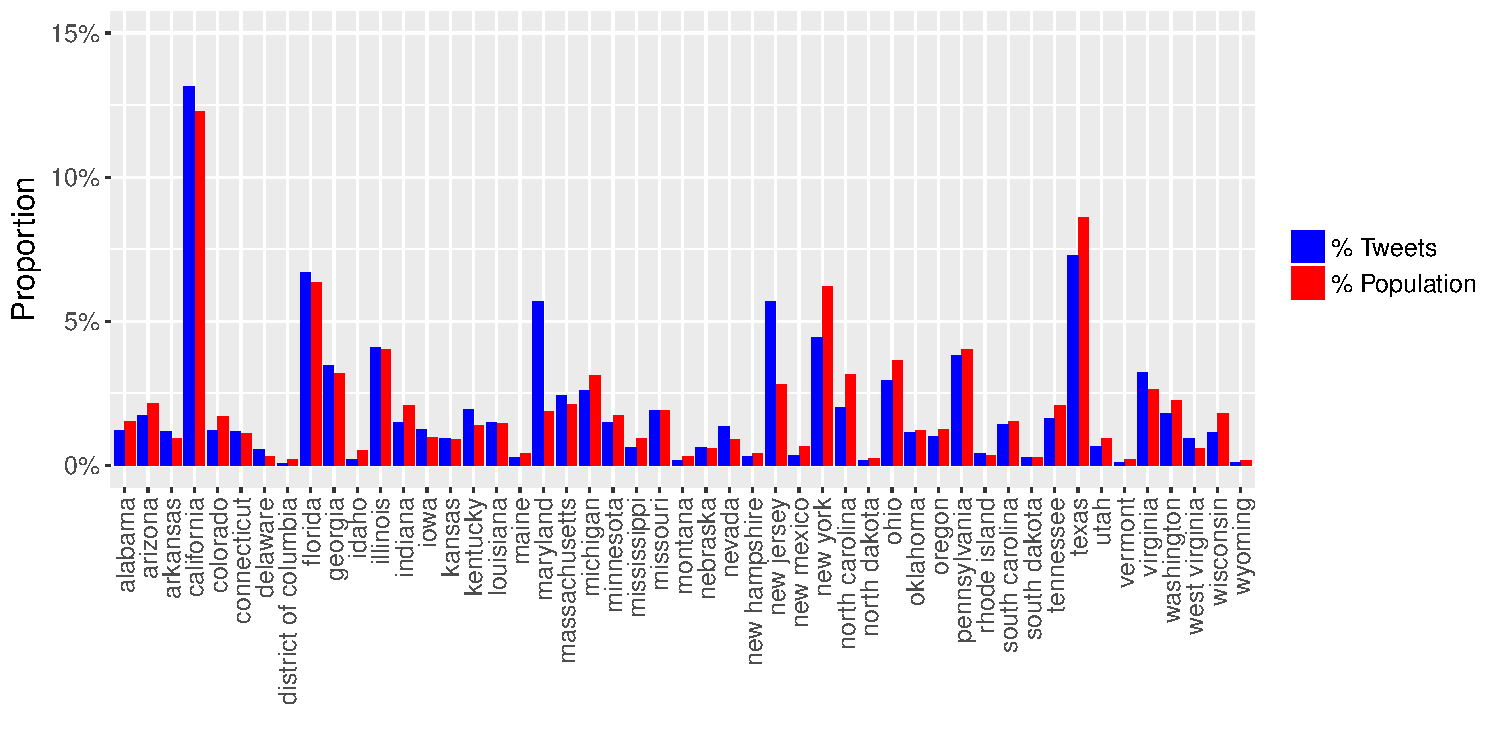
\includegraphics[width=1\linewidth]{15_activity_total_user_state_Twitter_full_aggregated.pdf}
  \caption{}
    \label{fig:tweets_state_full_user}
  \end{subfigure}
\caption{Relative number of tweets sent (a) and Twitter users (b) per state in the \texttt{all\_tweets} data set between 2011-03-05 and 2015-07-11 compared to each state's relative population size.}
\label{fig:tweets_state}
\end{figure}

\begin{figure}[htbp!]
\centering
 \begin{subfigure}[t]{0.6\textwidth}
  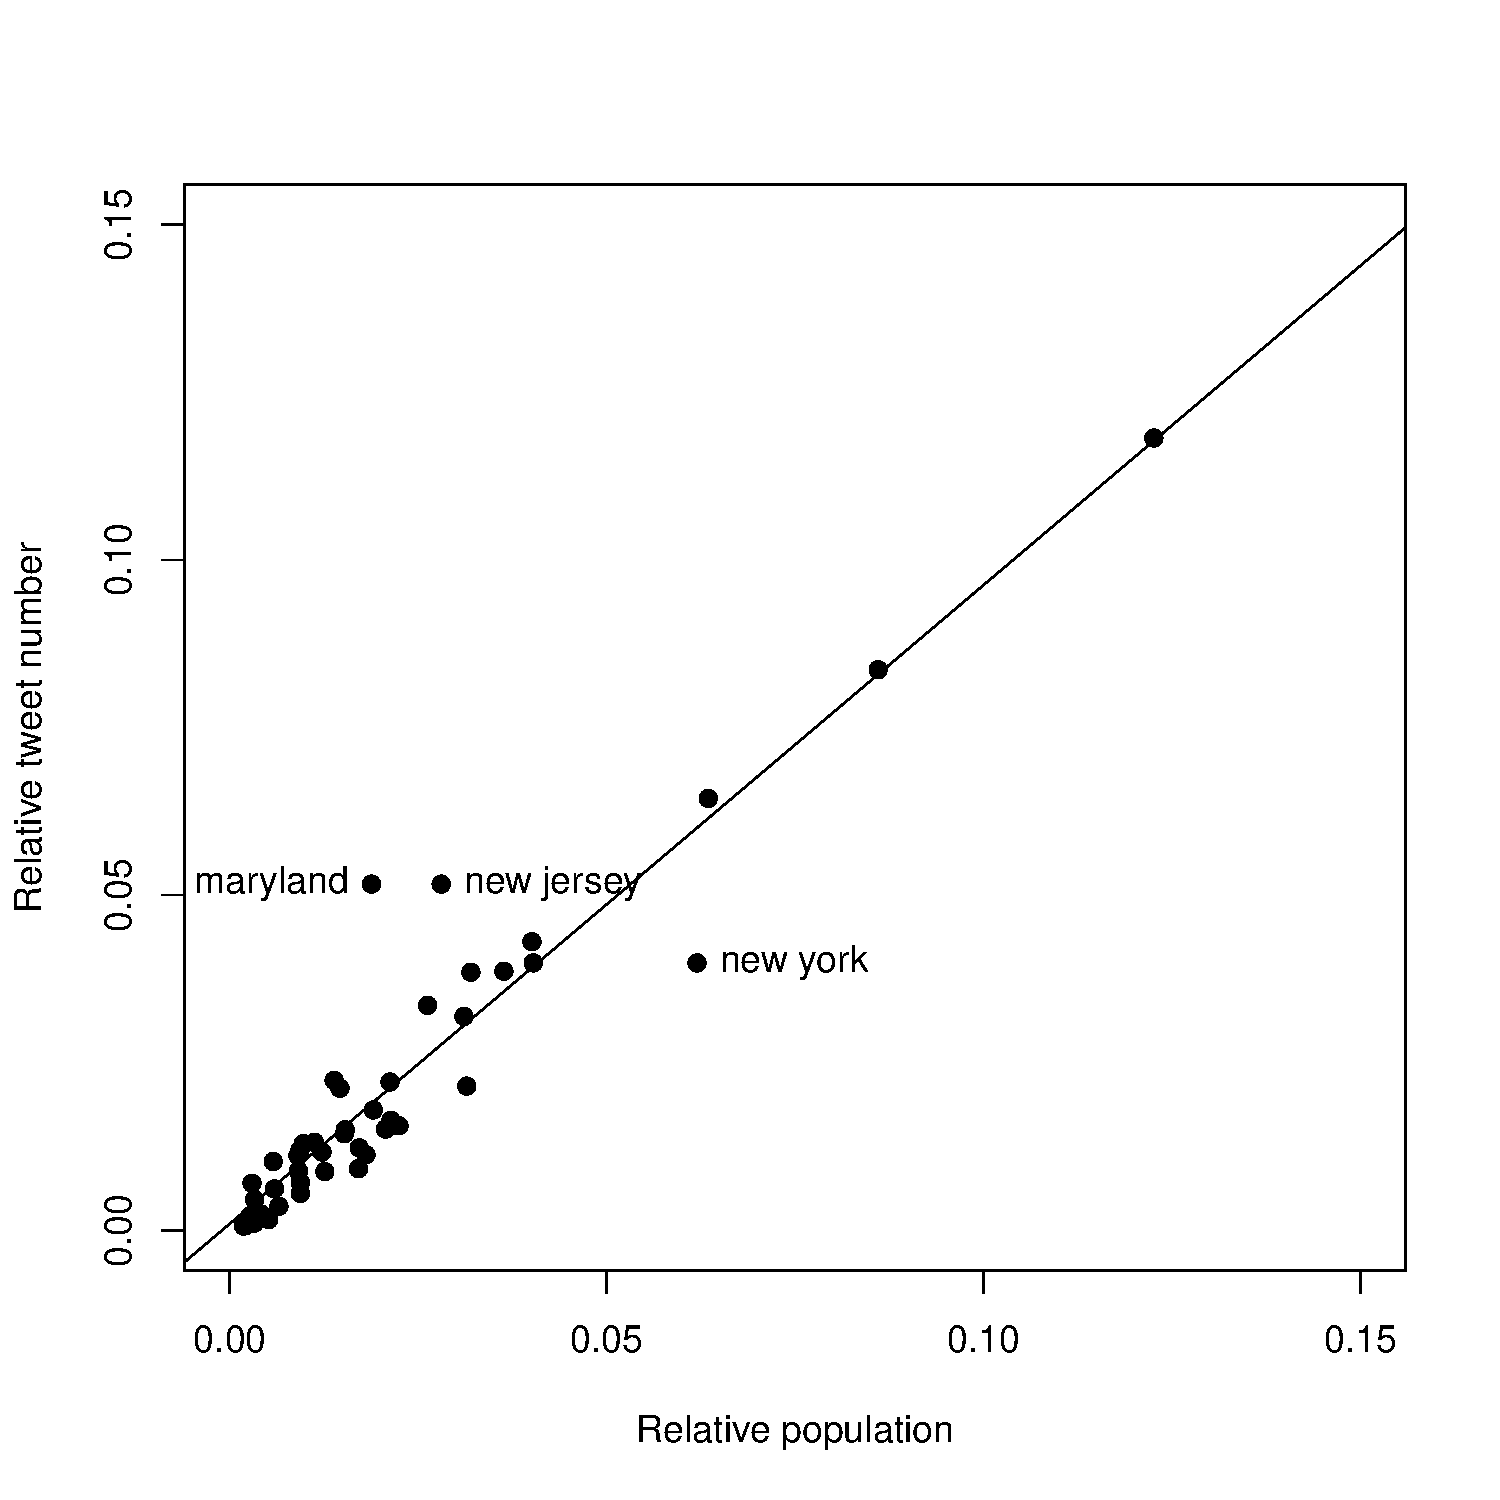
\includegraphics[width=1\linewidth]{16_ScatterTweetPop.pdf}
  \caption{}
  \label{fig:tweets_state_full_scatter}
  \end{subfigure}
  
  \begin{subfigure}[t]{0.6\textwidth}
  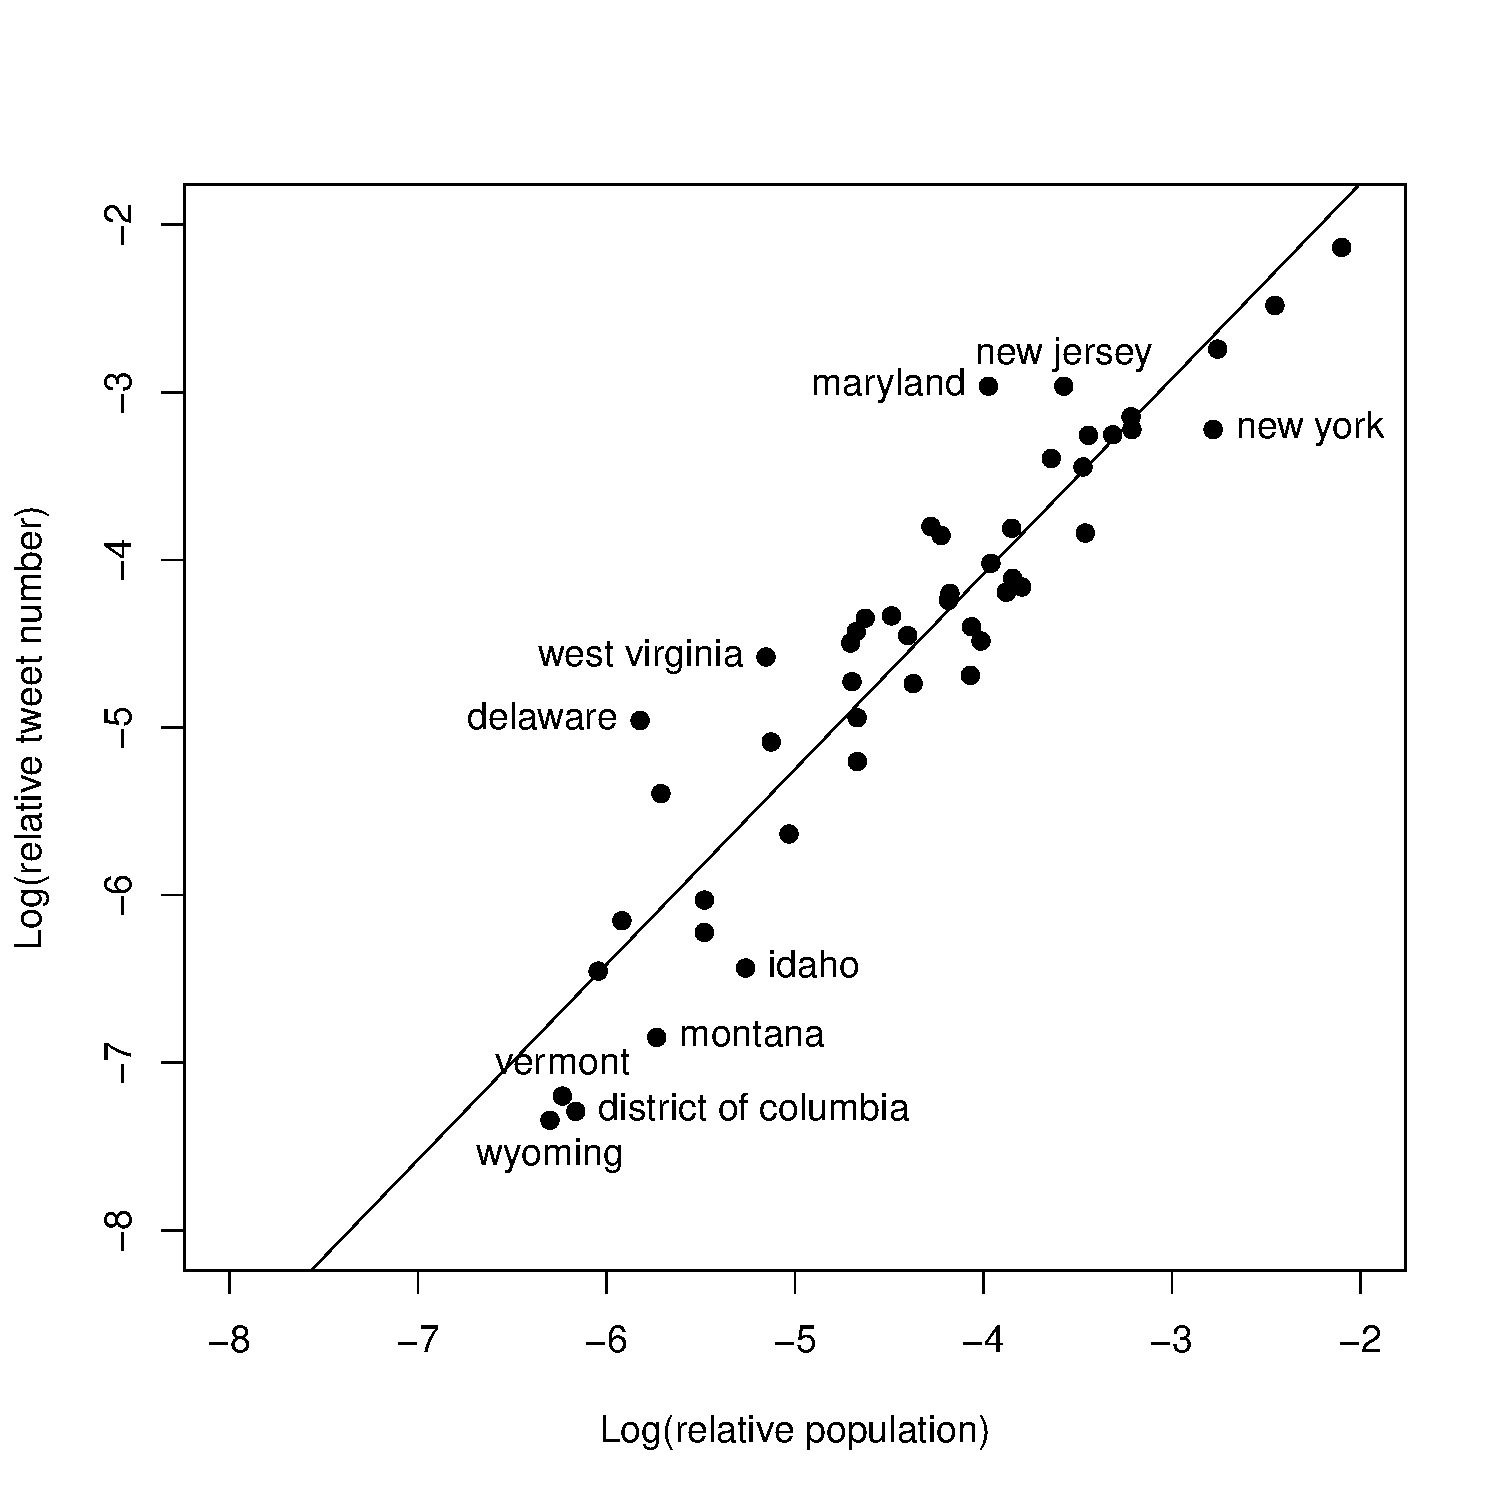
\includegraphics[width=1\linewidth]{17_ScatterTweetPop_log.pdf}
  \caption{}
  \label{fig:tweets_state_full_scatter_log}
  \end{subfigure}

\caption{Relative number of tweets sent per state in the \texttt{all\_tweets} data set between 2011-03-05 and 2015-07-11 plotted against each state's relative population size on a linear (a) and logartihmic scale (b). Some labels were removed to improve readability. The regression lines indicate the best linear fit with intercept = 0 and slope = 0.95 in (a) and intercept = 0.58 and slope = 1.16 in (b), respectively.}
\end{figure}

\begin{figure}[htbp!]
\centering
 \begin{subfigure}[t]{0.6\textwidth}
  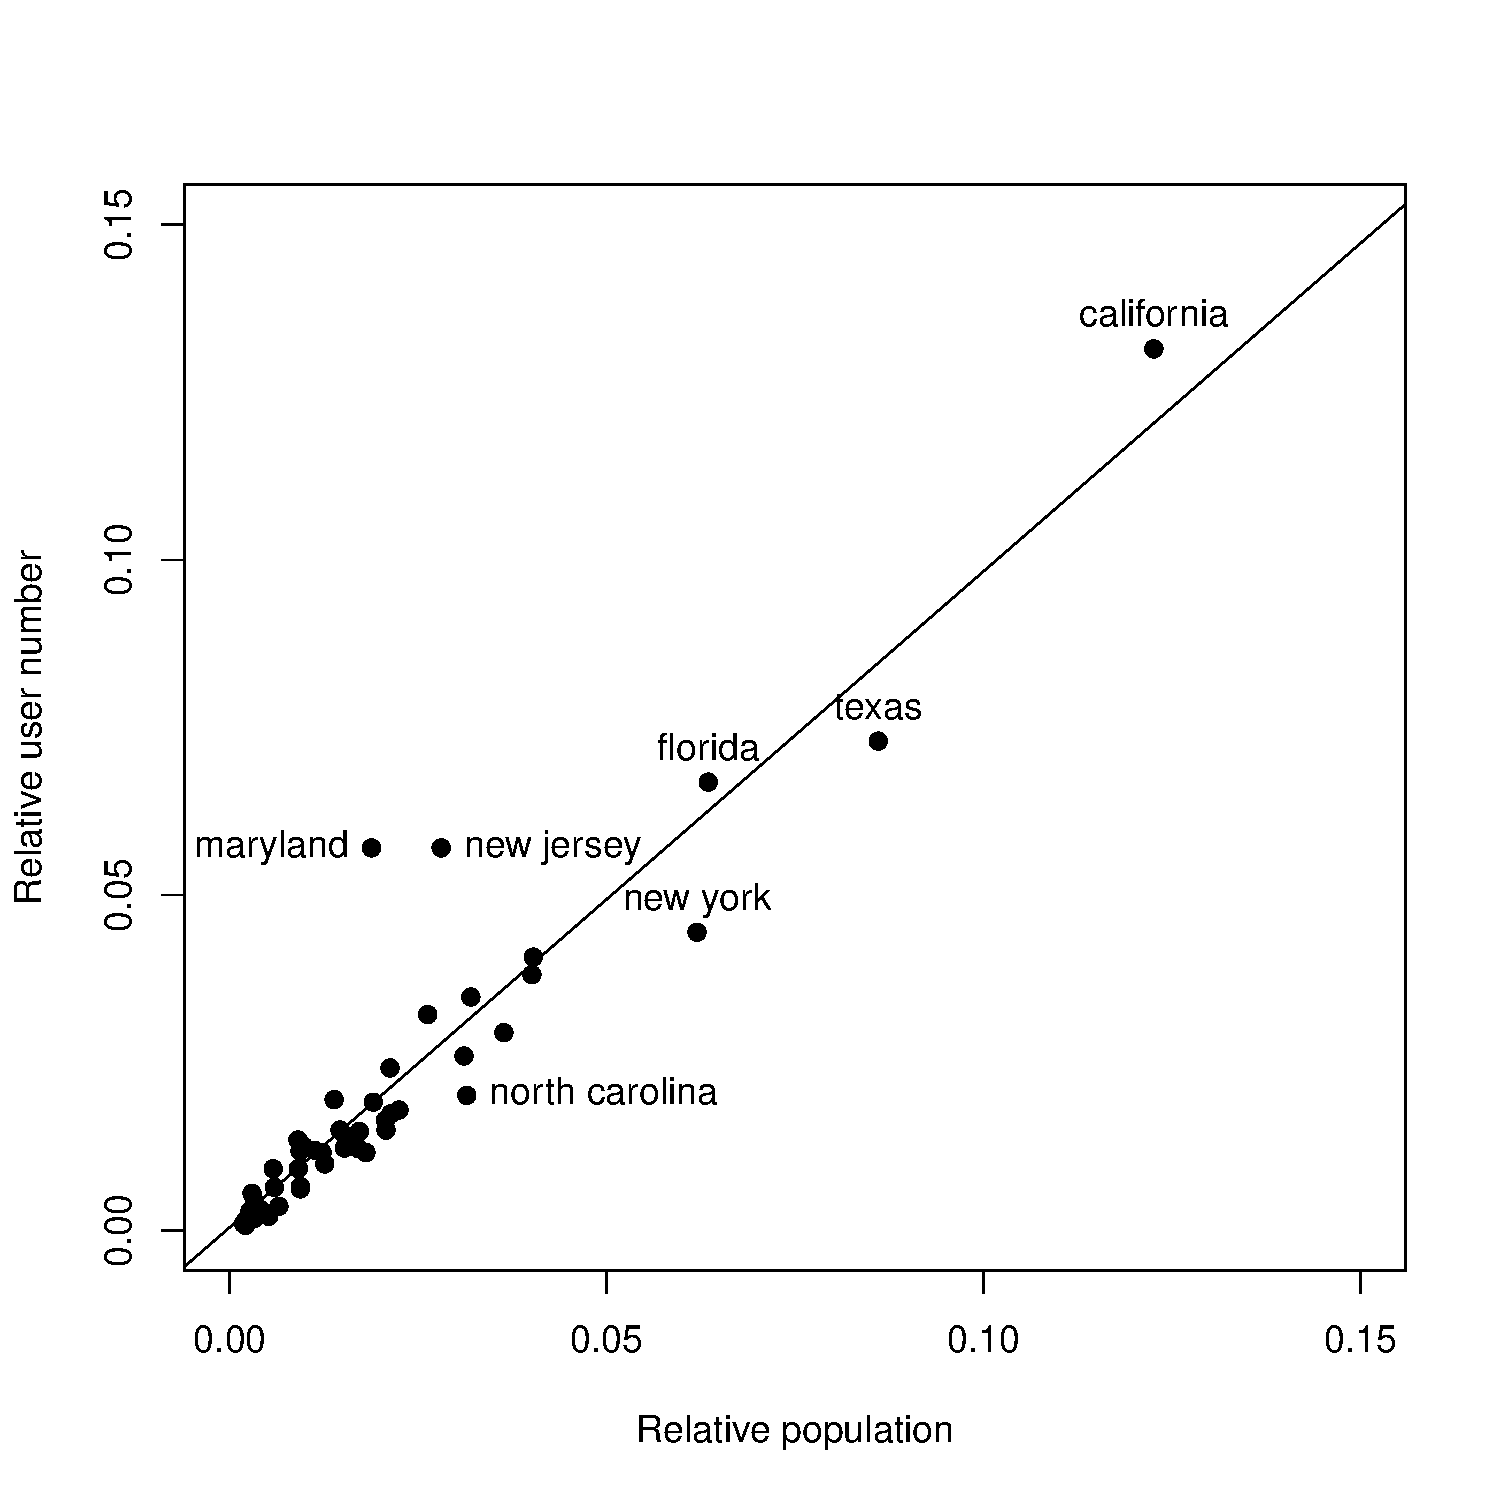
\includegraphics[width=1\linewidth]{18_ScatterTweetPop_user.pdf}
  \caption{}
  \label{fig:tweets_state_full_scatter_user}
  \end{subfigure}
  
  \begin{subfigure}[t]{0.6\textwidth}
  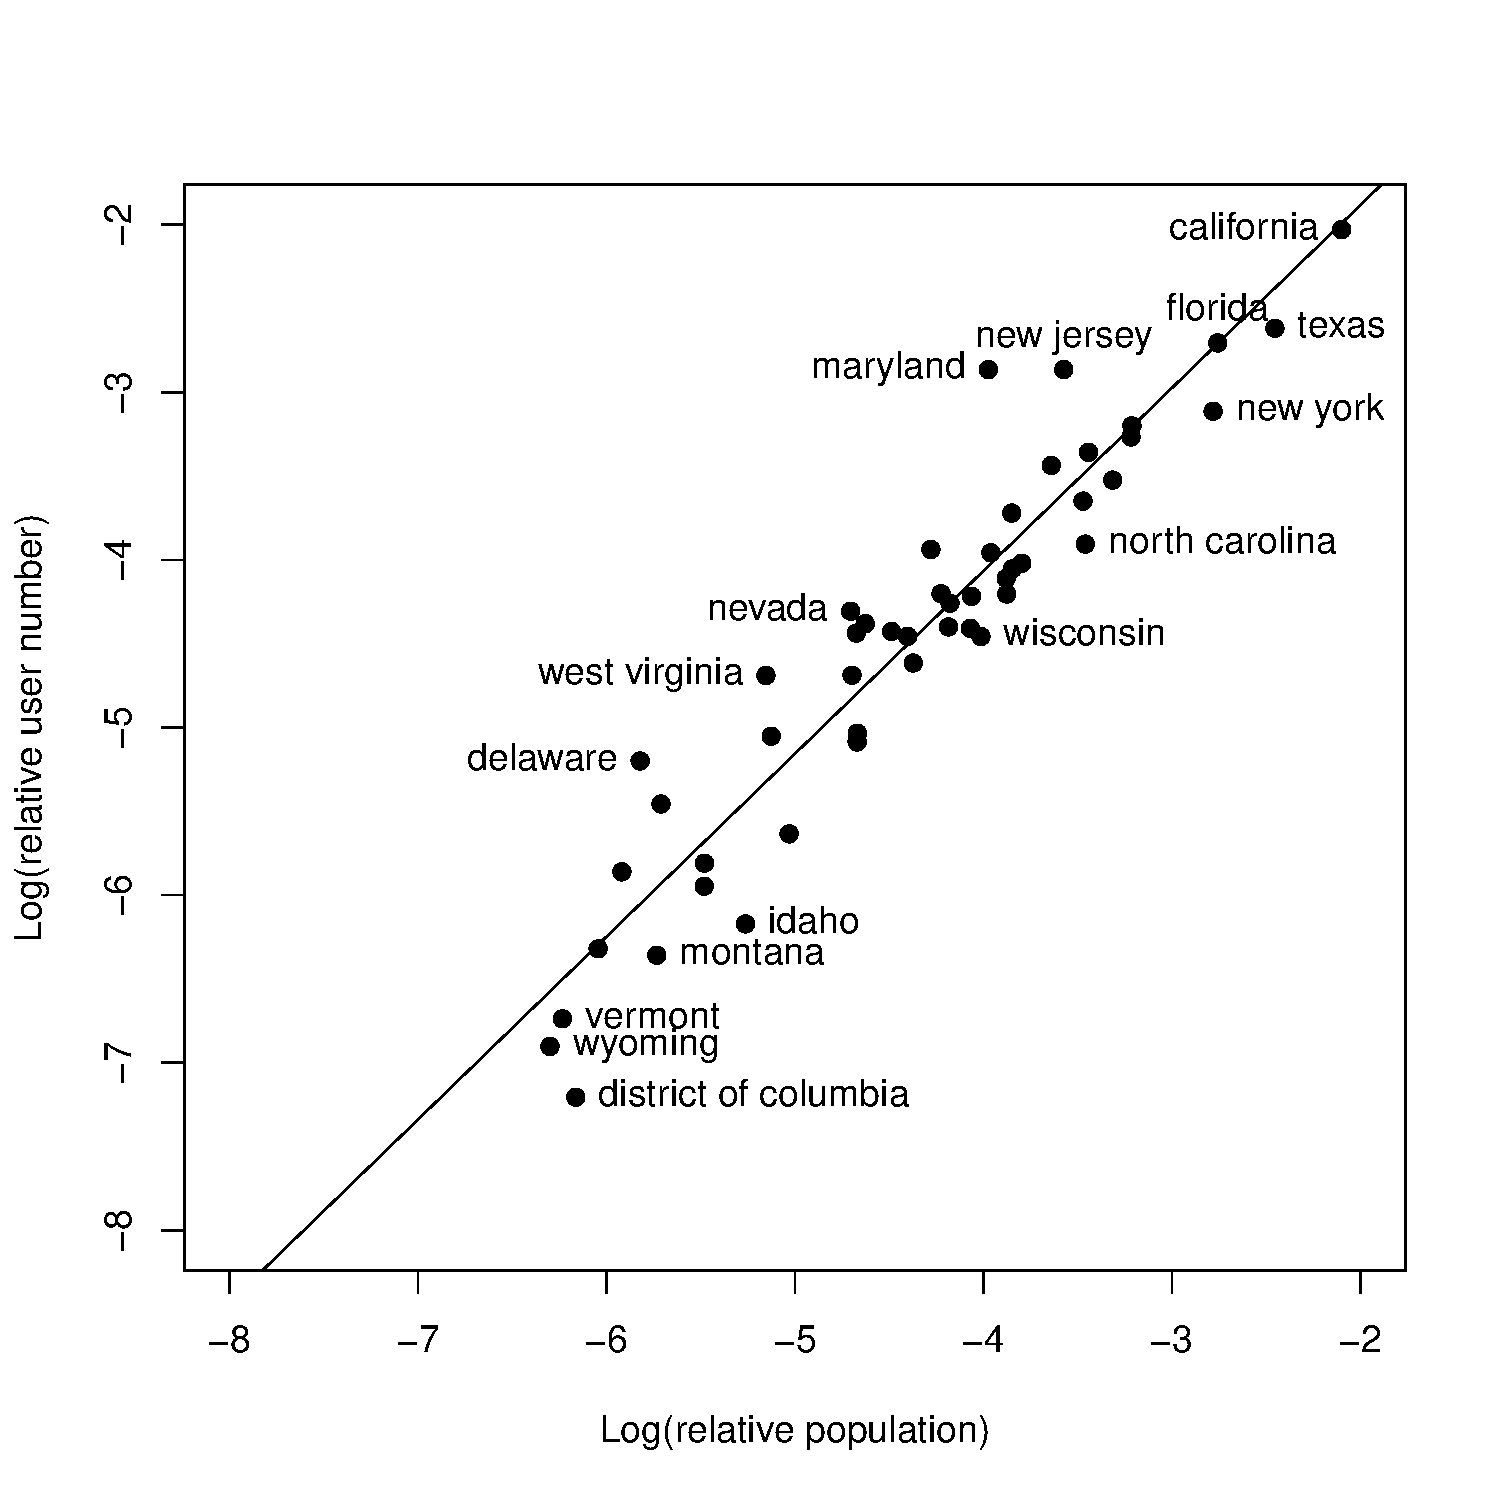
\includegraphics[width=1\linewidth]{19_ScatterTweetPop_user_log.pdf}
  \caption{}
  \label{fig:tweets_state_full_scatter_user_log}
  \end{subfigure}

\caption{Relative number of Twitter users per state in the \texttt{all\_tweets} data set between 2011-03-05 and 2015-07-11 plotted against each state's relative population size on a linear (a) and logartihmic scale (b). Some labels were removed to improve readability. The regression lines indicate the best linear fit with intercept = 0 and slope = 0.98 in (a) and intercept = 0.3 and slope = 1.09 in (b), respectively.}
\end{figure}

\begin{figure}[htbp!]
\centering
  \begin{subfigure}[t]{1\textwidth}
  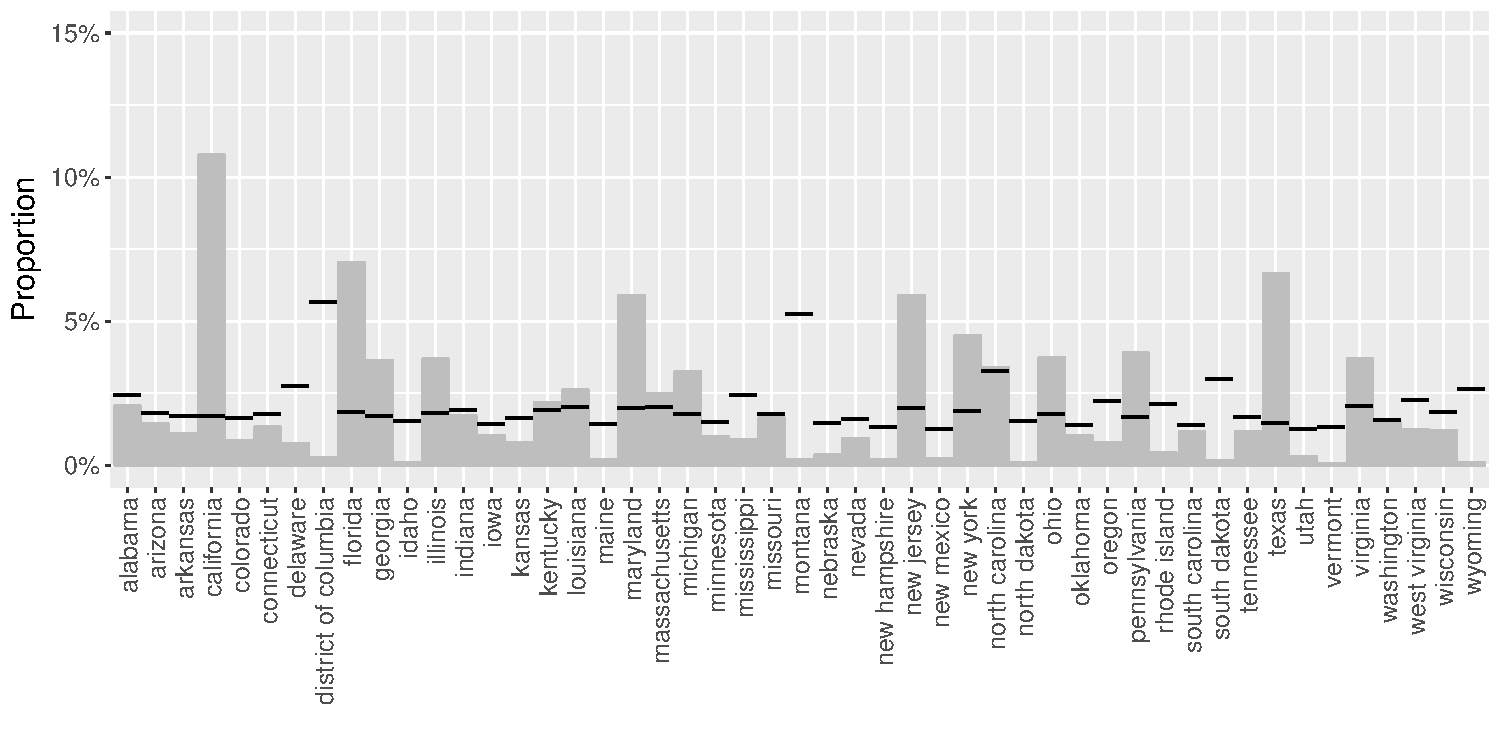
\includegraphics[width=1\linewidth]{20_activity_sick_statename_Twitter_full_aggregatedoverlay.pdf}
  \caption{}
  \end{subfigure}
\hfill
  \begin{subfigure}[t]{1\textwidth}
  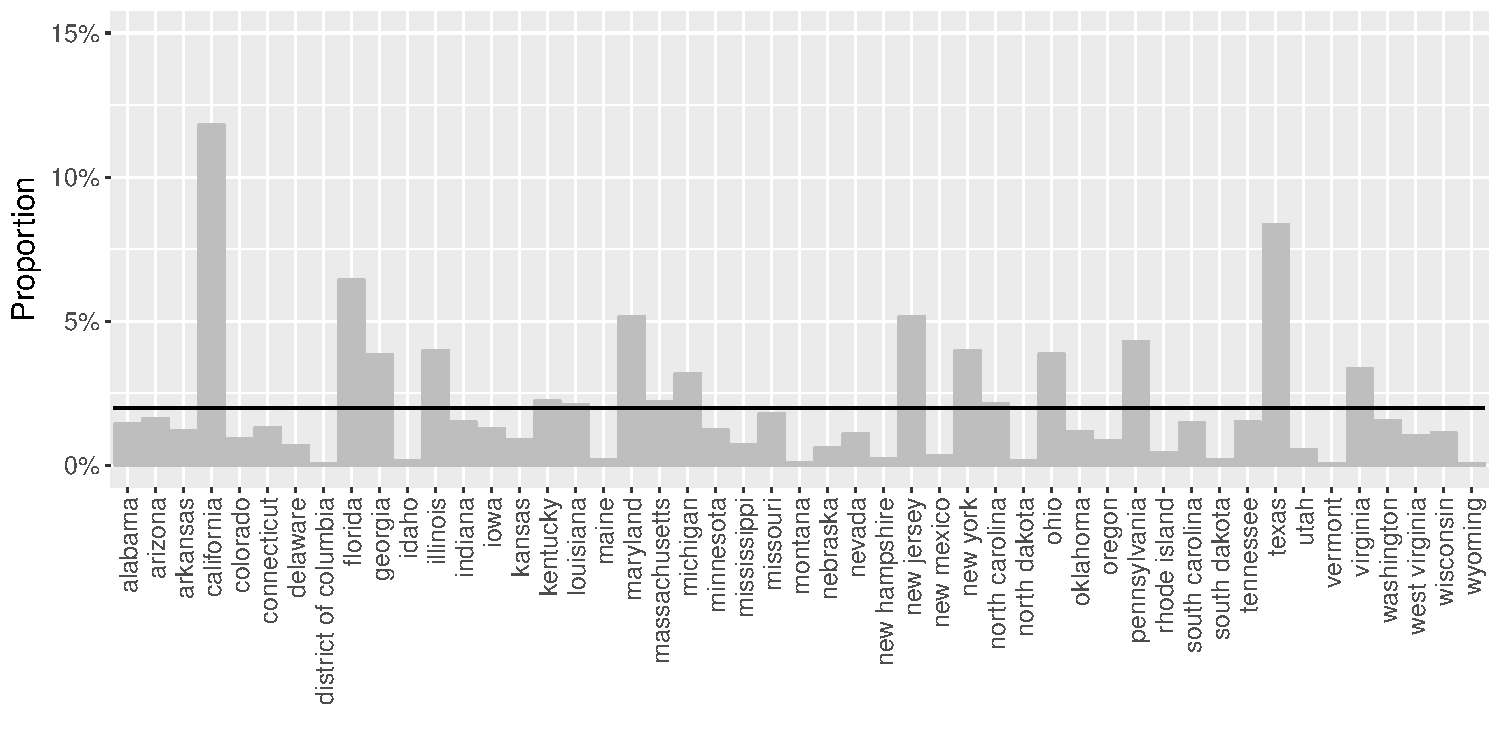
\includegraphics[width=1\linewidth]{21_activity_healthy_statename_Twitter_full_aggregatedoverlay.pdf}
  \caption{}
  \end{subfigure}
  
  \caption{Histograms of numbers of tweets sent from eeach state during the 208 weeks between 2011-03-05 and 2015-07-11 (bin size = 1 week). (a) shows only tweets labelled as ``sick"; (b) shows only tweets labelled as ``healthy" by the classifier. The grey bars indicate the relative number of sick or healthy tweets sent in each state without normalisation. The black lines indicate the relative number of sick or healthy tweets sent in each state normalised by the total amount of tweets sent that state.}
  \label{fig:tweets_state_healthy_sick}
\end{figure}

\begin{figure}[htbp!]
\centering
  \begin{subfigure}[t]{1\textwidth}
  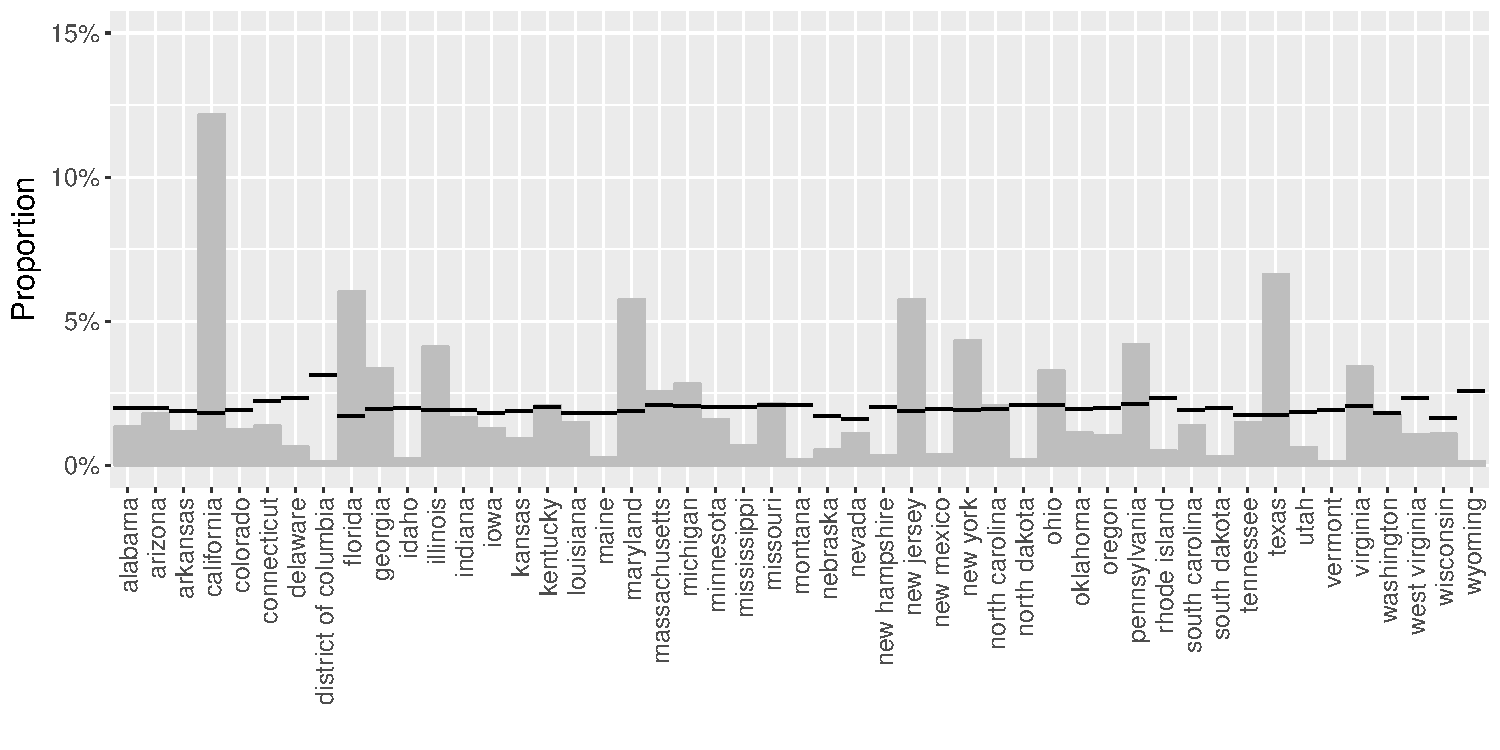
\includegraphics[width=1\linewidth]{22_activity_sick_user_statename_Twitter_full_aggregatedoverlay.pdf}
  \caption{}
  \end{subfigure}
\hfill
  \begin{subfigure}[t]{1\textwidth}
  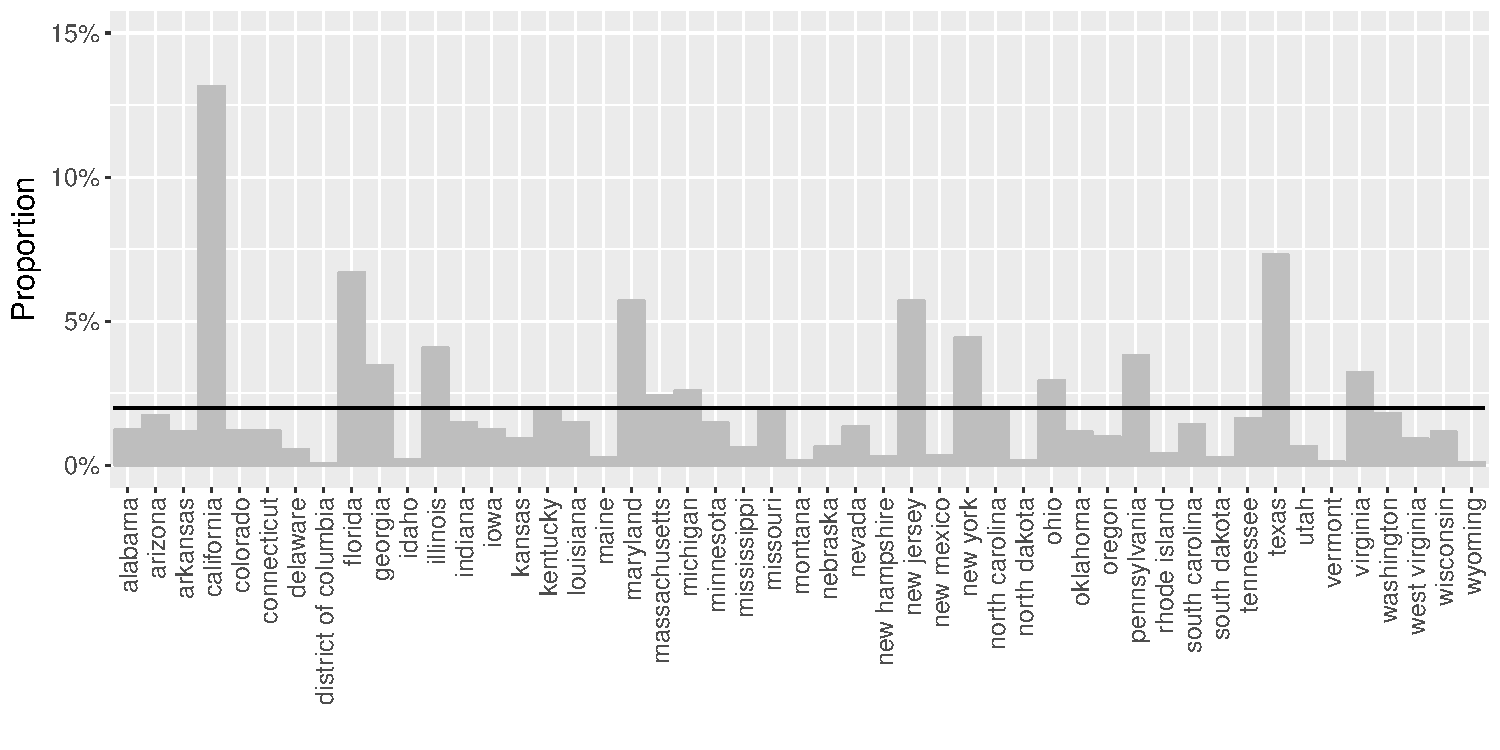
\includegraphics[width=1\linewidth]{23_activity_healthy_user_statename_Twitter_full_aggregatedoverlay.pdf}
  \caption{}
  \end{subfigure}
  \caption{Histograms of numbers of users active in each state during the 208 weeks between 2011-03-05 and 2015-07-11 (bin size = 1 week). (a) shows only users who sent at least one tweet labelled as ``sick"; (b) shows only users who were never classified as ``sick" during the whole study period. The grey bars indicate the relative number of sick or healthy users active in each state without normalisation. The black lines indicate the relative number of sick or healthy users active in each state normalised by the total amount of tweets sent in that week.}
  \label{fig:tweets_state_healthy_sick_user}
\end{figure}

\subsection{Comparing the flu classifier results with CDC ILI rates}
\label{sec:comp_cdc}

In order to assess the validity of the ILI predictions provided by the flu classifier, I compared the results from the Twitter classifier with the official ILI reports from the CDC on the national, regional and state level(extracted using the ``cdcfluview" package \citep{cdcfluview}).

In a first step, I simply compared the official CDC ILI percentage data on the national level with the relative number of tweets labelled as ``sick" per week and the relative number of sick users per week, respectively. As can be seen from Figure~\ref{fig:naive_comparison_CDC_twitter}, the relative results from the Twitter classifer are an order of magnitude smaller than the official ILI data from the CDC.

In order to make them directly comparable to each other, I normalised both time series by the total sum of relative tweets numbers and ILI percentages, respectively. Hence, the percentual values shown in Figure~\ref{fig:cdc_tw_comp_nat_ma1} do not represent weekly ILI percentage, but rather the percentual proportion of the relative number of tweets and the ILI percentages, respectively, of a given week within the whole 208 week study period (In other words: The percentages of each week add up to a 100\%, just like the histogram values shown in Figures~\ref{fig:tweets_seasonal_healthy_sick_user}--\ref{fig:tweets_seasonal_full}). Since the fluctuations in the Twitter data were very high, I plotted the data again after applying a two-week (Figure~\ref{fig:cdc_tw_comp_nat_ma2}) and four-week (Figure~\ref{fig:cdc_tw_comp_nat_ma4}) moving average smoother, using the ``forecast" package \citep{forecast}. This reduced the overall fluctuations a bit, but did not particularly improve the fit with the CDC curve. I did the same for each of the ten CDC flu surveillance regions (Figure~\ref{fig:cdc_tw_comp_regs_ma4}). The situation improves slightly if we use the relative amount of sick users per week (as opposed to the relative amount of sick tweets per week), as can be seen  from Figures~\ref{fig:cdc_tw_comp_nat_user_ma1}, \ref{fig:cdc_tw_comp_nat_user} and \ref{fig:cdc_tw_comp_regs_ma4_user}. In both cases, however, the correlation between the relative ILI estimates based on Twitter data and the official CDC data were abysmal (Spearman's Rho was 0.0077 and 0.0077 for tweet- and user-based four-week average curves, respectively). 

\begin{figure}[htbp!]
\centering
  \begin{subfigure}[t]{1\textwidth}
  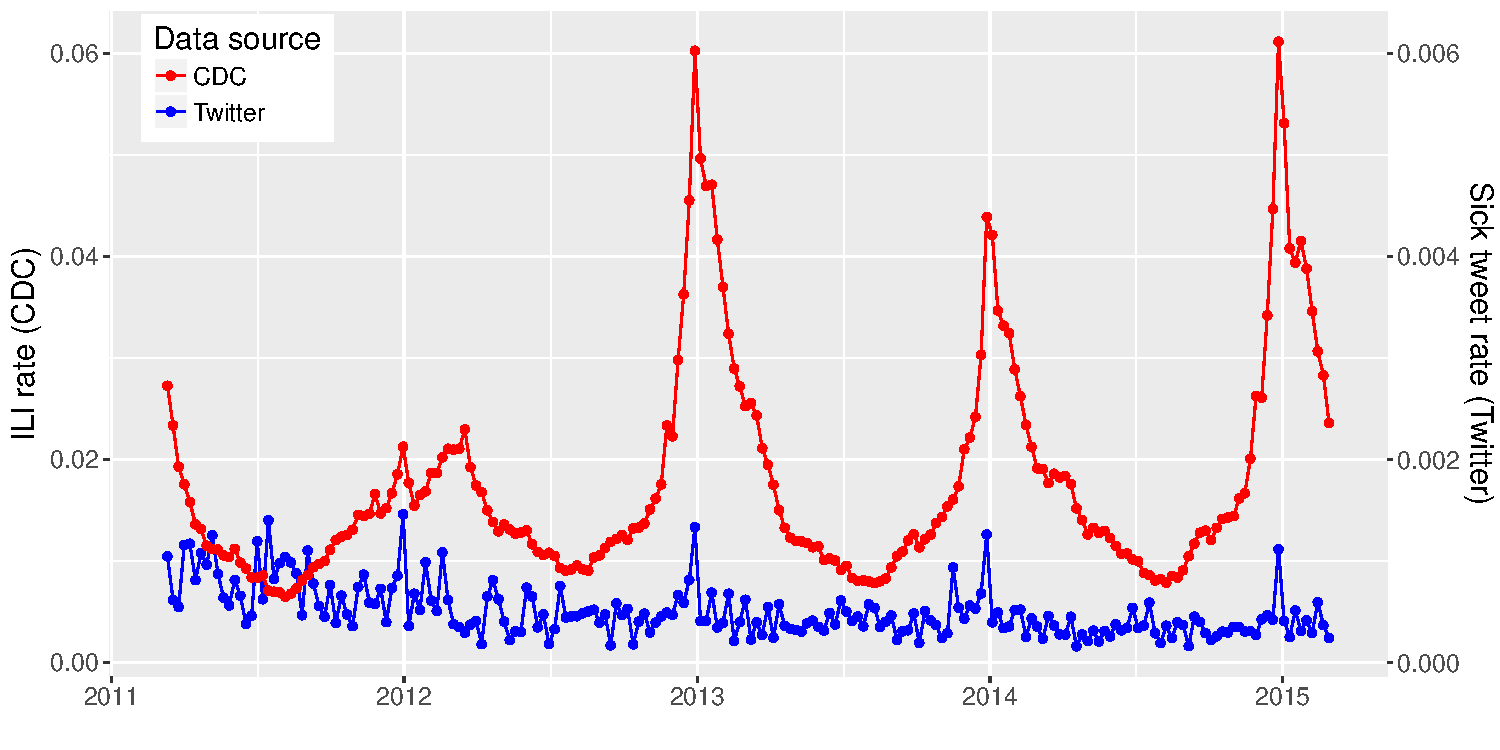
\includegraphics[width=1\linewidth]{24_cdc_twitter_comp_nat_raw.pdf}
  \caption{}
  \end{subfigure}
\hfill
  \begin{subfigure}[t]{1\textwidth}
  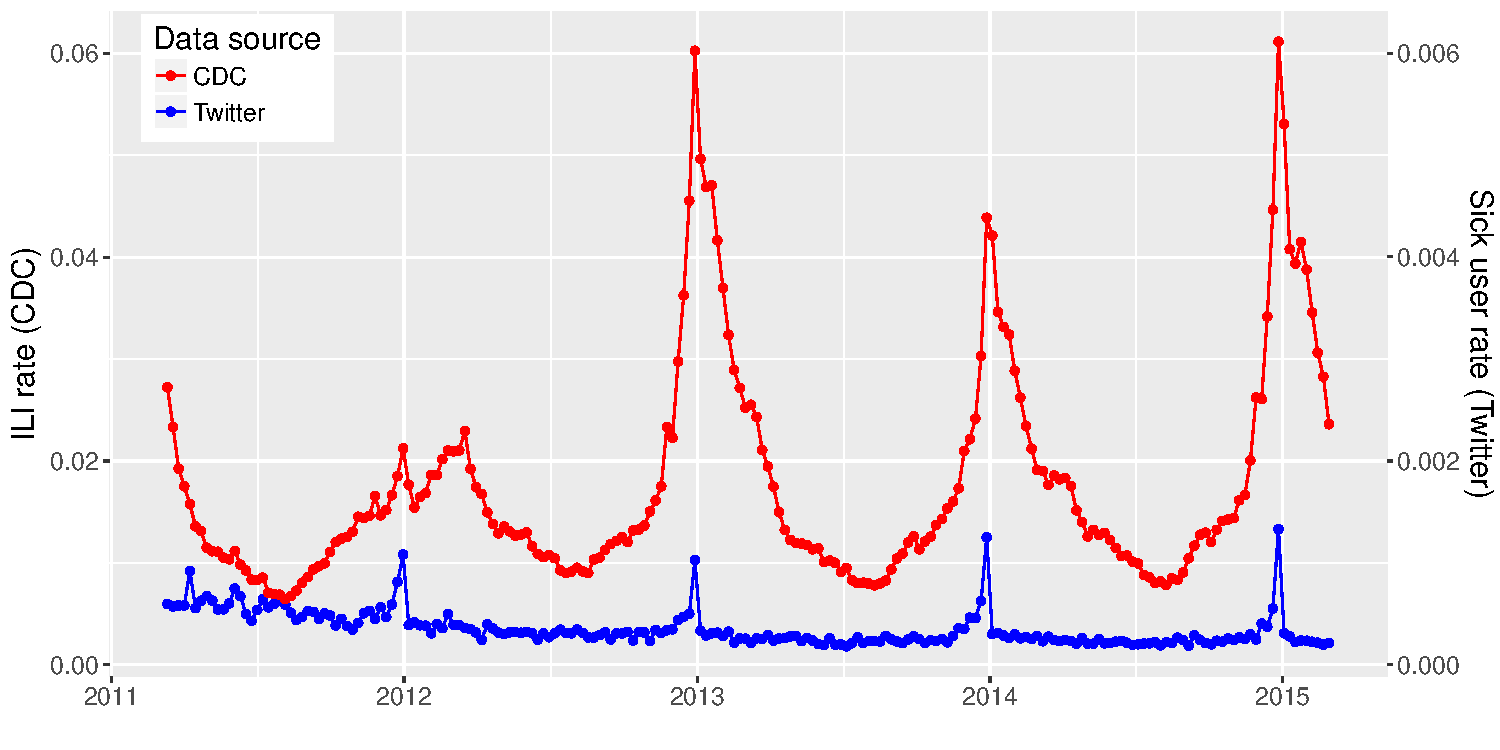
\includegraphics[width=1\linewidth]{25_cdc_twitter_comp_nat_raw_user.pdf}
  \caption{}
  \end{subfigure}
  \caption{Comparison between weekly CDC ILI rates (red) and the results from the Twitter classifier (blue). (a) shows the relative amount of tweets labelled as sick during a given week. (b) shows the relative amount of users labelled as ``sick" by the classifier. Not that the Twitter rates are given in order of per mille of all tweets and users, respectively (right y-axis), while CDC ILI rates ar given in order of percent of all patients visiting ILINet outpatient clinics (left y-axis).}
  \label{fig:naive_comparison_CDC_twitter}
\end{figure}

\begin{figure}[htbp!]
  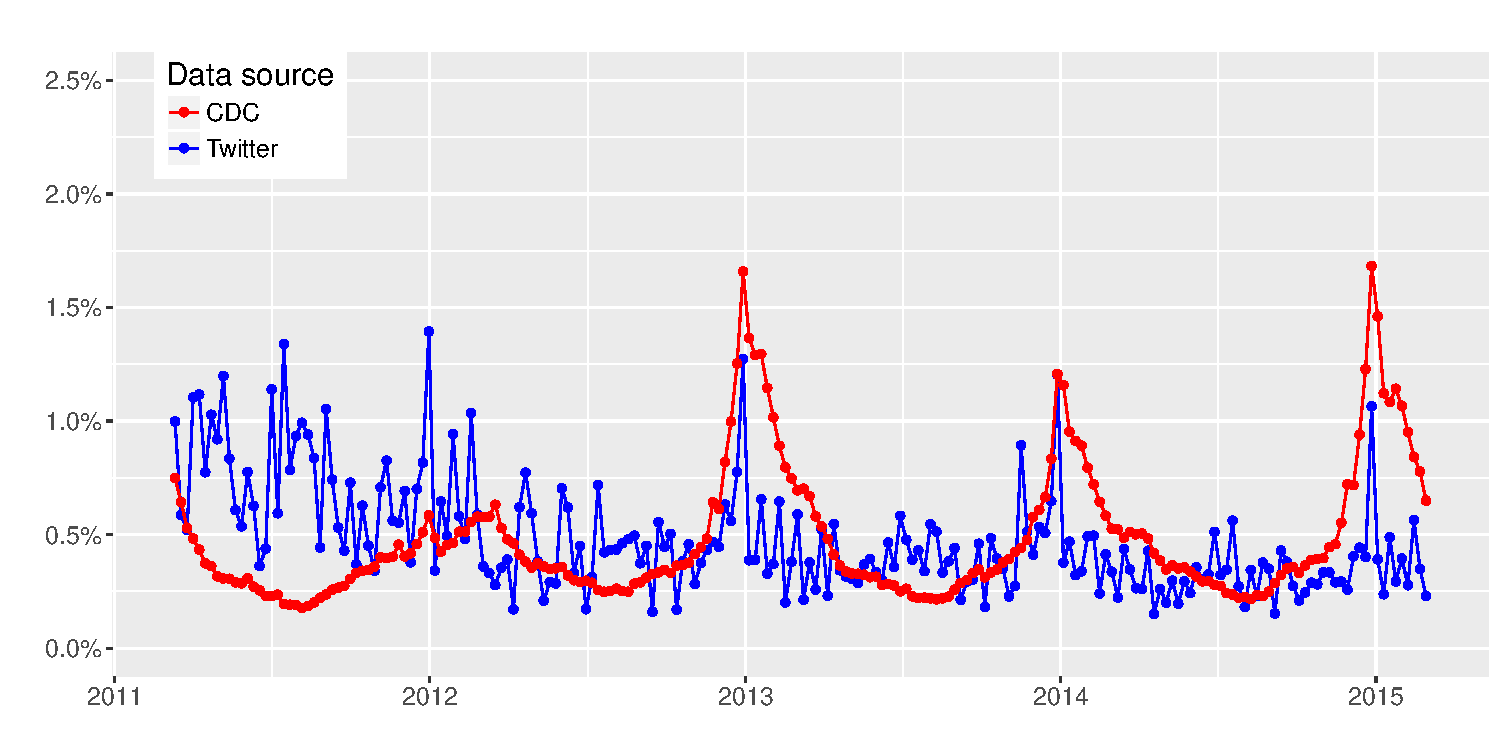
\includegraphics[width=1\linewidth]{26_cdc_twitter_comp_nat_ma1.pdf}
  \caption{}
  \caption{Comparison between weekly CDC ILI rates (red) and the relative amount of tweets labelled as ``sick" from the Twitter flu classifier (blue). The data has been normalised in order to make them comparable, i.e. the percentages do not represent weekly ILI percentages, but instead sum up to a 100\% over the whole time period.}
    \label{fig:cdc_tw_comp_nat_ma1}
\end{figure}

\begin{figure}[htbp!]
\centering
  \begin{subfigure}[t]{1\textwidth}
  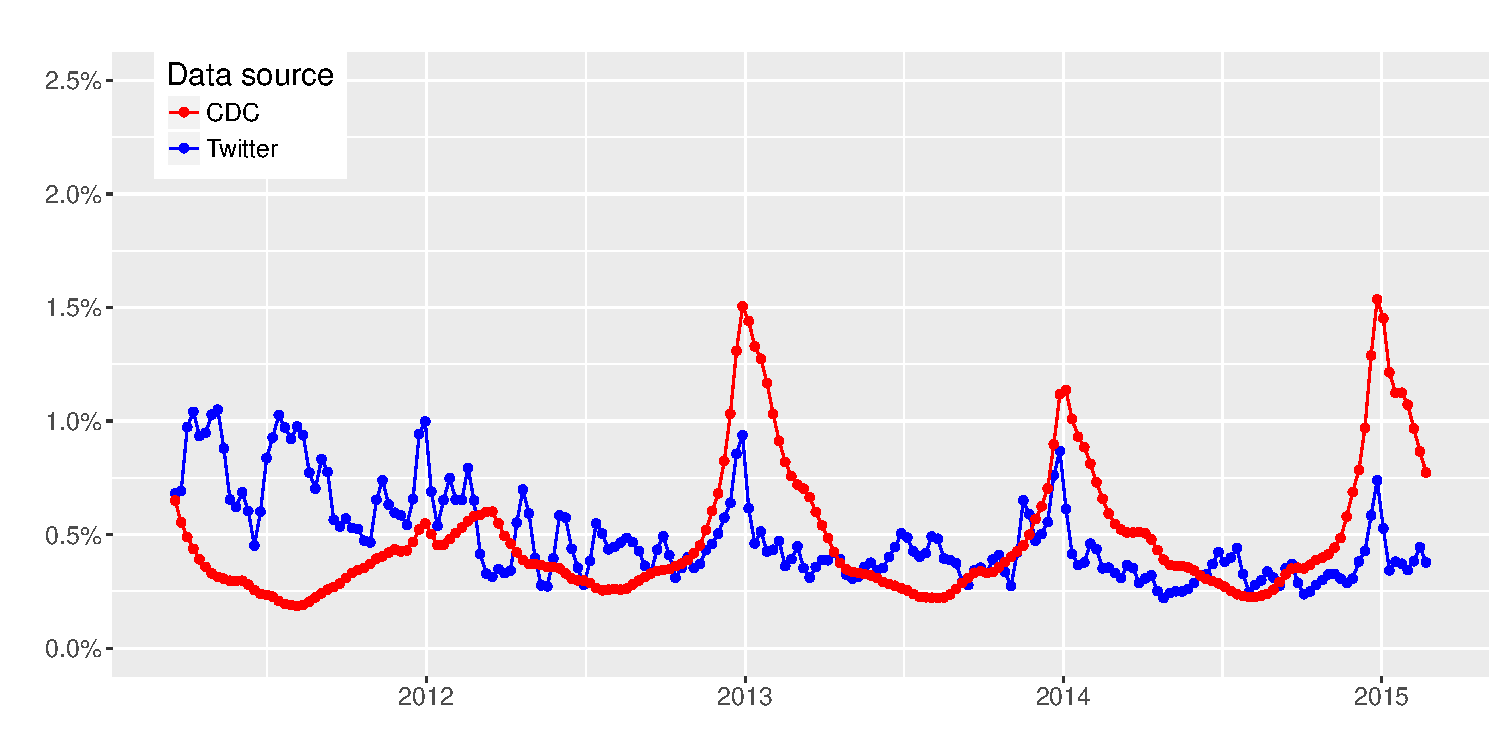
\includegraphics[width=1\linewidth]{27_cdc_twitter_comp_nat_ma2.pdf}
  \caption{}
  \label{fig:cdc_tw_comp_nat_ma2}
  \end{subfigure}
  
  \begin{subfigure}[t]{1\textwidth}
  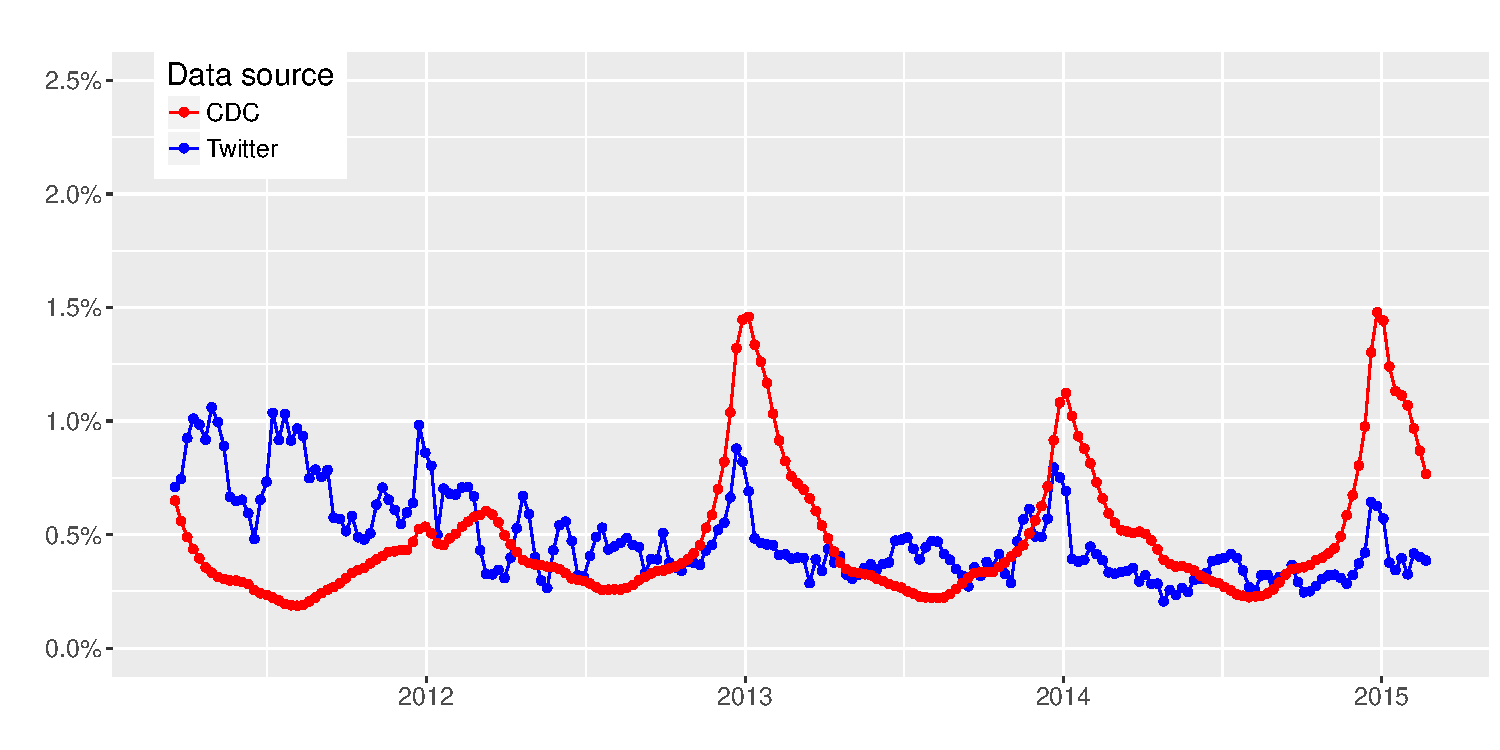
\includegraphics[width=1\linewidth]{28_cdc_twitter_comp_nat_ma4.pdf}
  \caption{}
  \label{fig:cdc_tw_comp_nat_ma4}
  \end{subfigure}
  \caption{Comparison between weekly CDC ILI rates (red) and the relative amount of tweets labelled as ``sick" from the Twitter flu classifier (blue) after applying a two-week moving average smoother (a) and after applying a four-week moving average smoother (b), respectively. The data has been normalised in order to make them comparable, i.e. the percentages do not represent weekly ILI percentages, but instead sum up to a 100\% over the whole time period.}
  \label{fig:cdc_tw_comp_nat_tot}
\end{figure}

\begin{figure}[htbp!]
\centering
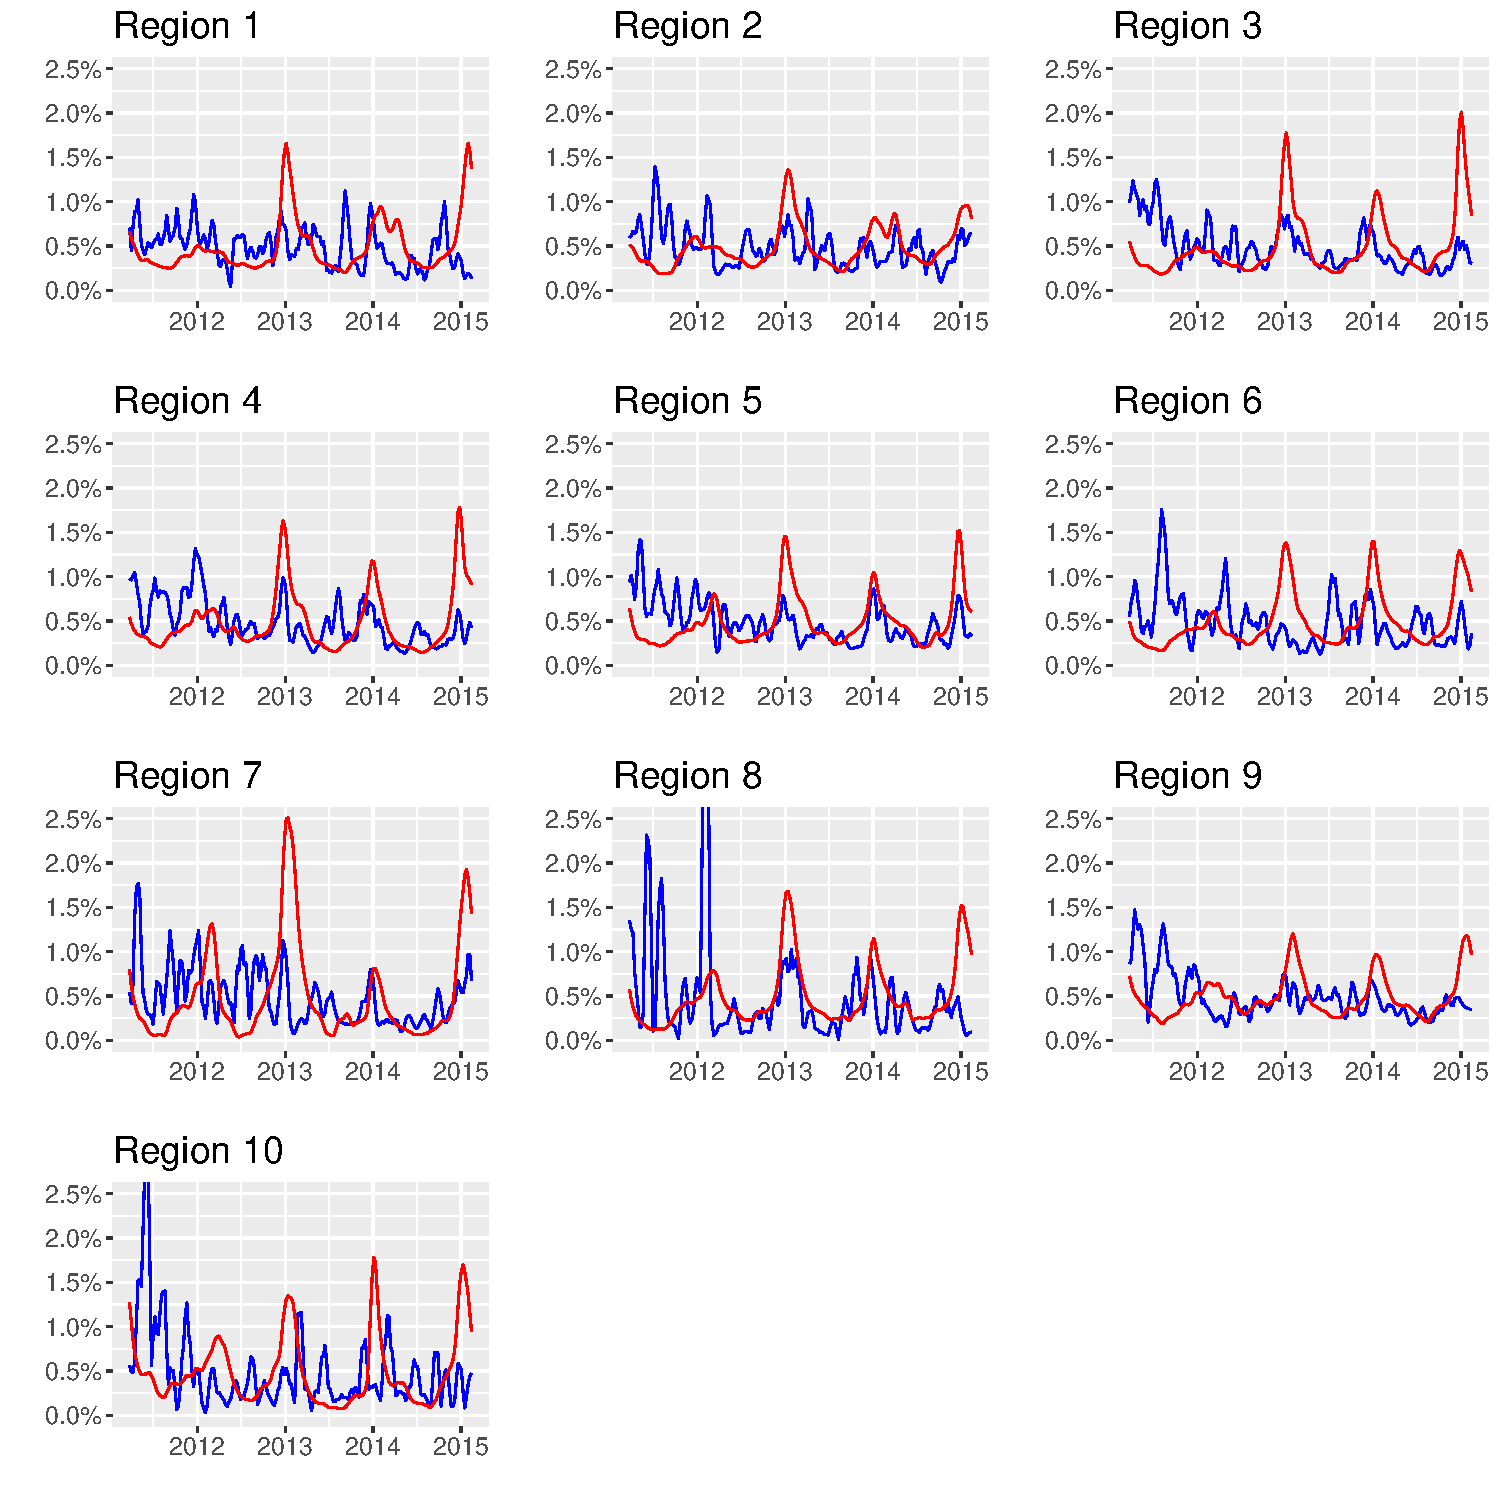
\includegraphics[width=1\linewidth]{29_cdc_twitter_comp_regs_ma4.pdf}
\caption{Relative number of tweets sent within each CDC ILI surveillance region per week (blue) compared with weekly ILI percentages in those regions (red). Data has been normalised and processed with a four-week moving average smoother. Note that Region 2 contains ``Puerto Rico" and ``Virgin Islands", Region 9 contains ``Hawaii" and Region 10 contains ``Alaska", all of which are missing from the Twitter data set.}
\label{fig:cdc_tw_comp_regs_ma4}
\end{figure}

\begin{figure}[htbp!]
  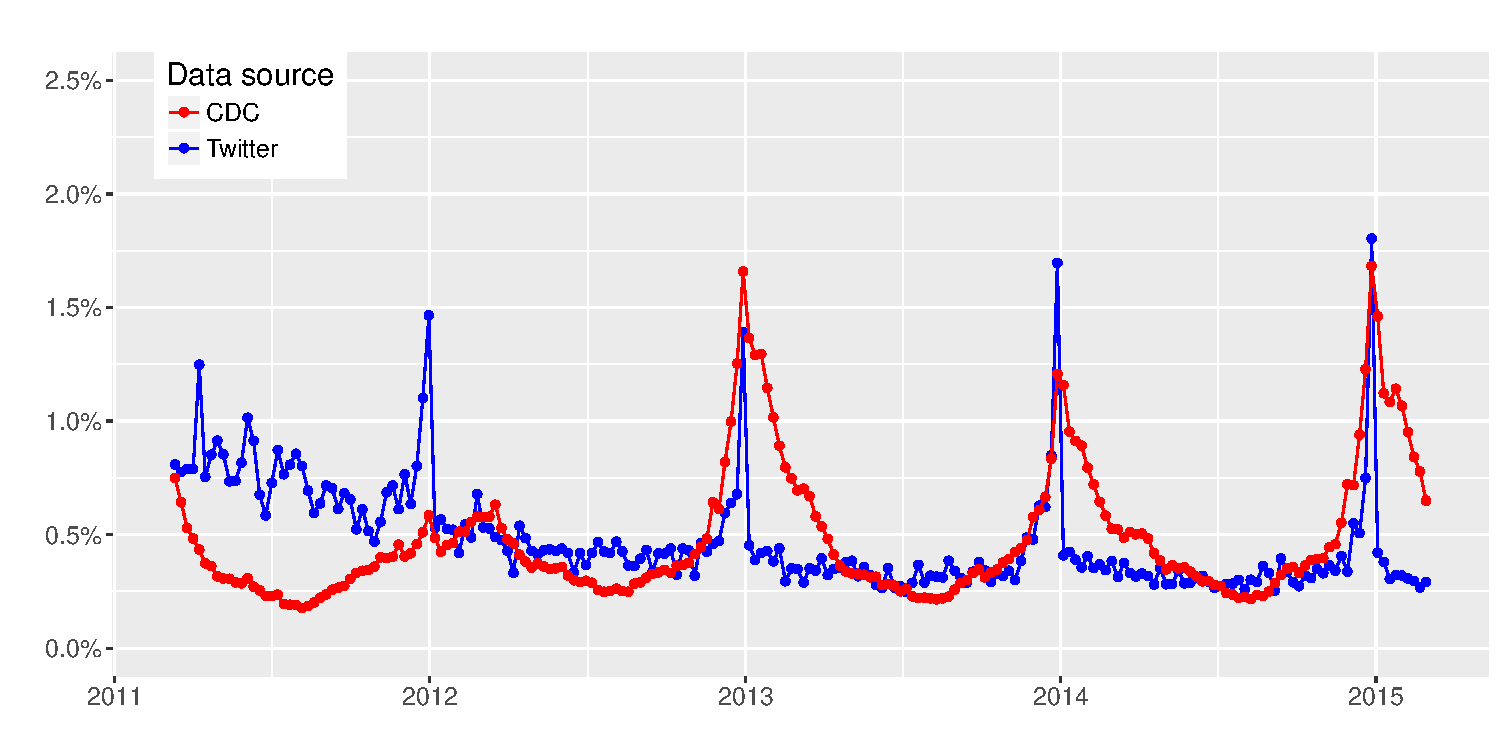
\includegraphics[width=1\linewidth]{30_cdc_twitter_comp_nat_ma1_user.pdf}
  \caption{}
  \caption{Comparison between weekly CDC ILI rates (red) and the relative amount of users who sent at least one tweet classified as ``sick" from the Twitter flu classifier (blue) during a specific week The data has been normalised in order to make them comparable, i.e. the percentages do not represent weekly ILI percentages, but instead sum up to a 100\% over the whole time period.}
    \label{fig:cdc_tw_comp_nat_user_ma1}
\end{figure}

\begin{figure}[htbp!]
\centering
  \begin{subfigure}[t]{1\textwidth}
  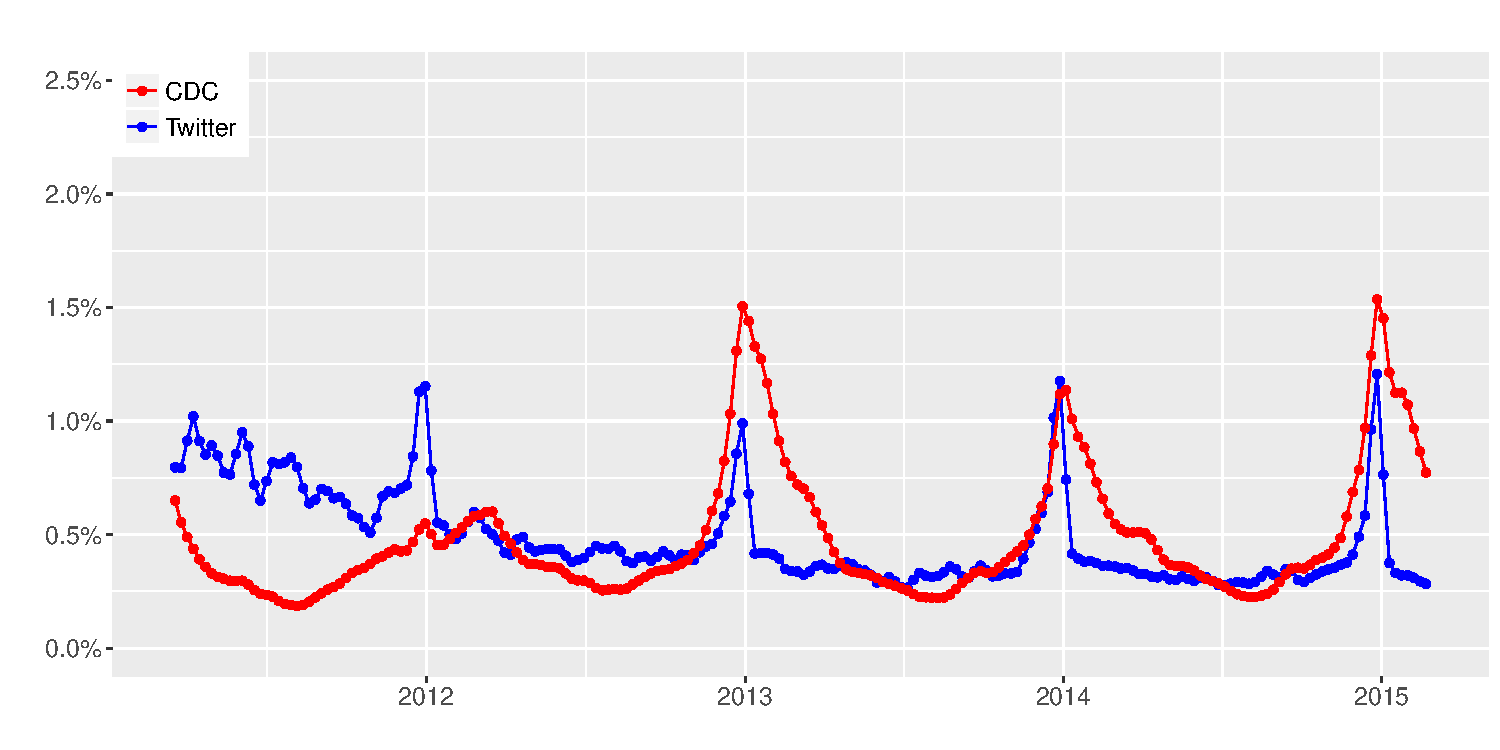
\includegraphics[width=1\linewidth]{31_cdc_twitter_comp_nat_ma2_user.pdf}
  \caption{}
  %\label{cdc_tw_comp_nat_ma2_user}
  \end{subfigure}
  
  \begin{subfigure}[t]{1\textwidth}
  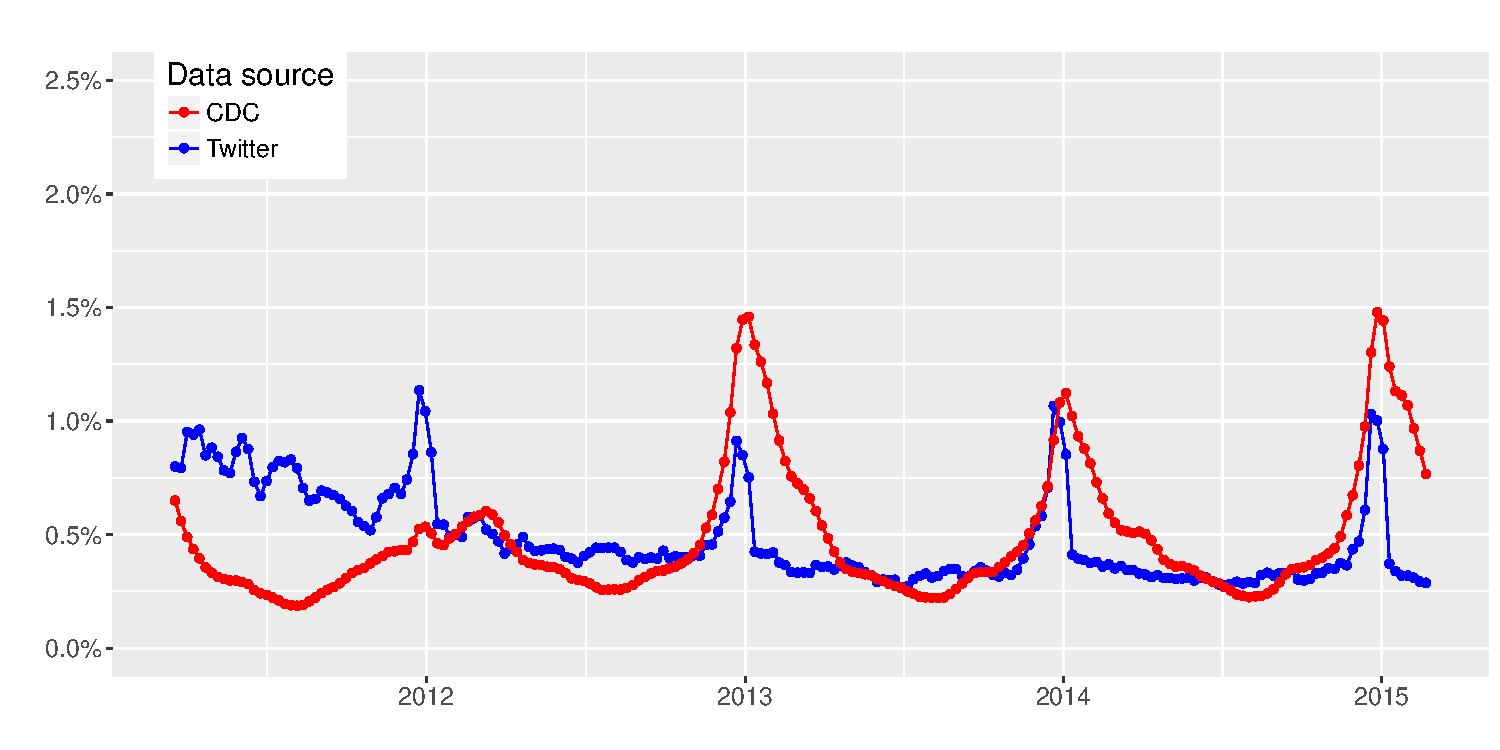
\includegraphics[width=1\linewidth]{32_cdc_twitter_comp_nat_ma4_user.pdf}
  \caption{}
  %\label{cdc_tw_comp_nat_ma4_user}
  \end{subfigure}
  \caption{Comparison between weekly CDC ILI rates (red) and the relative amount of users who sent at least one tweet classified as ``sick" from the Twitter flu classifier (blue) during a specific week (a) and after applying a four-week moving average smoother (b), respectively. The data has been normalised in order to make them comparable, i.e. the percentages do not represent weekly ILI percentages, but instead sum up to a 100\% over the whole time period.}
  \label{fig:cdc_tw_comp_nat_user}
\end{figure}

\begin{figure}[htbp!]
\centering
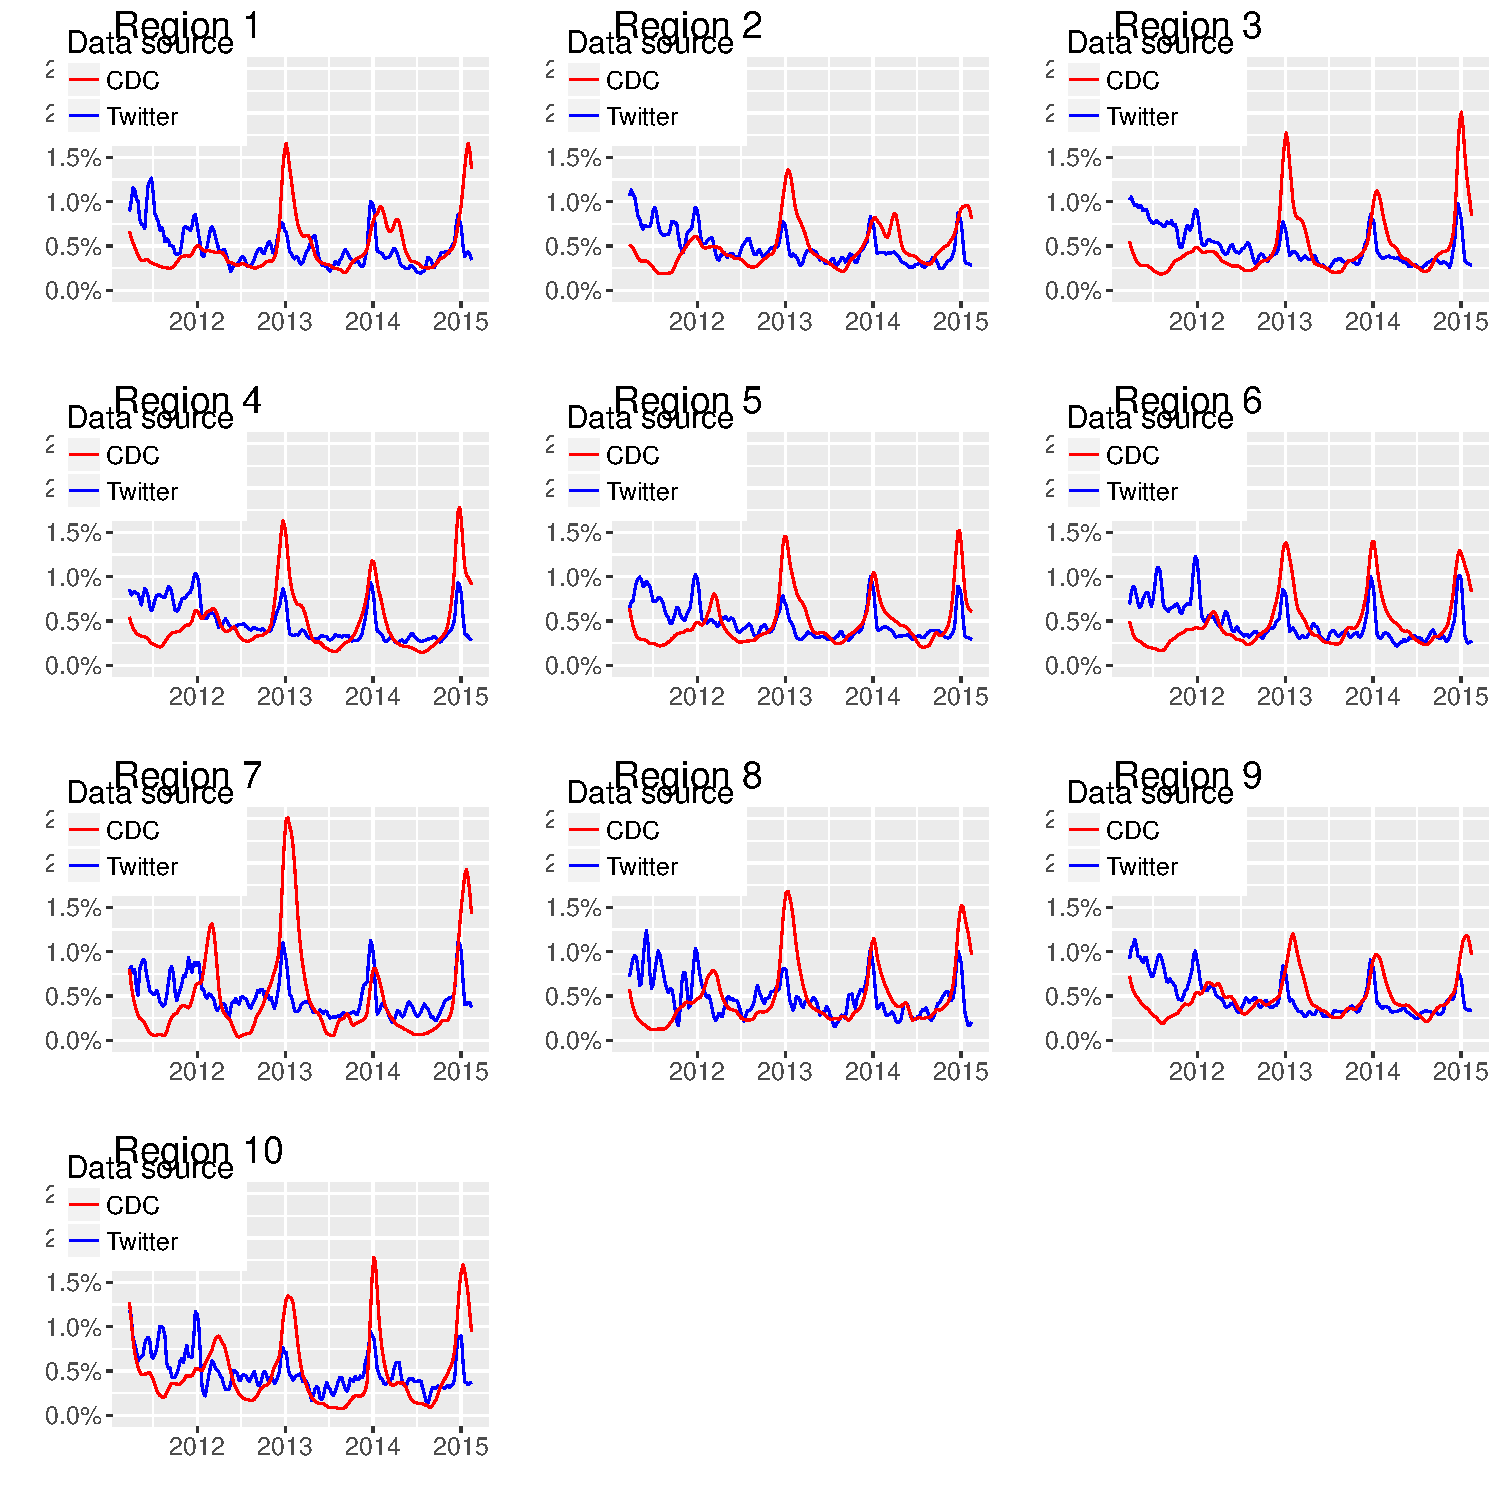
\includegraphics[width=1\linewidth]{33_cdc_twitter_comp_regs_ma4_user.pdf}
\caption{Relative number of users who sent at least one tweet labelled as ``sick" within each CDC ILI surveillance region per week (blue) compared with weekly ILI percentages in those regions (red). Data has been normalised and processed with a four-week moving average smoother. Note that Region 2 contains ``Puerto Rico" and ``Virgin Islands", Region 9 contains ``Hawaii" and Region 10 contains ``Alaska", all of which are missing from the Twitter data set.}
\label{fig:cdc_tw_comp_regs_ma4_user}
\end{figure}

\subsection{Comparing classifier results with CDC activity levels}
\label{sec:comp_cdc_ac}
Next, I attempted to reduce the fluctations and increase the comparibility with the CDC data by grouping the percentual values into one of ten activity levels inspired by the CDC's same grouping used for reporting.

The CDC differentiates between ten different ILI activity levels which represent the deviation relative to the ILI baseline values. The activity levels compare the mean reported percent of visits due to ILI for the current week to the ILI baseline based on the number of reported ILI cases during non-influenza weeks, which are defined as weeks with less than 2\% of reported patient visits due to ILI. More precisely, the baseline is calculated by averaging the percentages of recorded ILI patients during non-influenza weeks for the previous three seasons and then adding two standard deviations \citep{cdc_surveillance_2016}.

An activity level of 1 corresponds to values that are below the baseline, level 2 corresponds to an ILI percentage less than 1 standard deviation above the baseline, level 3 corresponds to ILI more than 1, but less than 2 standard deviations above the baseline, and so on, with an activity level of 10 corresponding to ILI 8 or more standard deviations above the baseline \citep{cdc_surveillance_2016}.
  
Since a similar threshold does not exist for the Twitter data, I simply used the relative number of tweets labelled as ``sick" during weeks outside the flu season (June to September; seasonal flu activity can begin as early as October and continue to occur as late as May) as source to calculate yearly baseline values during off-season weeks. I then used these baseline values to calculate the weekly activity levels according to the rationale describe above. Figure~\ref{fig:cdc_tw_comp_nat_ac_sick} and Figure~\ref{fig:cdc_tw_comp_regs_ac_sick} shows the comparison on the national and regional level, respectively. I then did the same using the relative number of sick users (as opposed to sick tweets) instead (Figure~\ref{fig:cdc_tw_comp_nat_ac_sick_user} and Figures~\ref{fig:cdc_tw_comp_regs_ac_sick_user}). Note that the Twitter data available to me only spanned the time period between 2011 and 2015. In order not too lose too many years worth of data to the baseline calculation, I only calculated the baseline based on the off-season weeks directly preceding a specific flu season (as opposed to calculating the baseline based on the off-season weeks of the three preceding weeks).\clearpage

\begin{figure}[htbp!]
\centering
  \begin{subfigure}[t]{1\textwidth}
  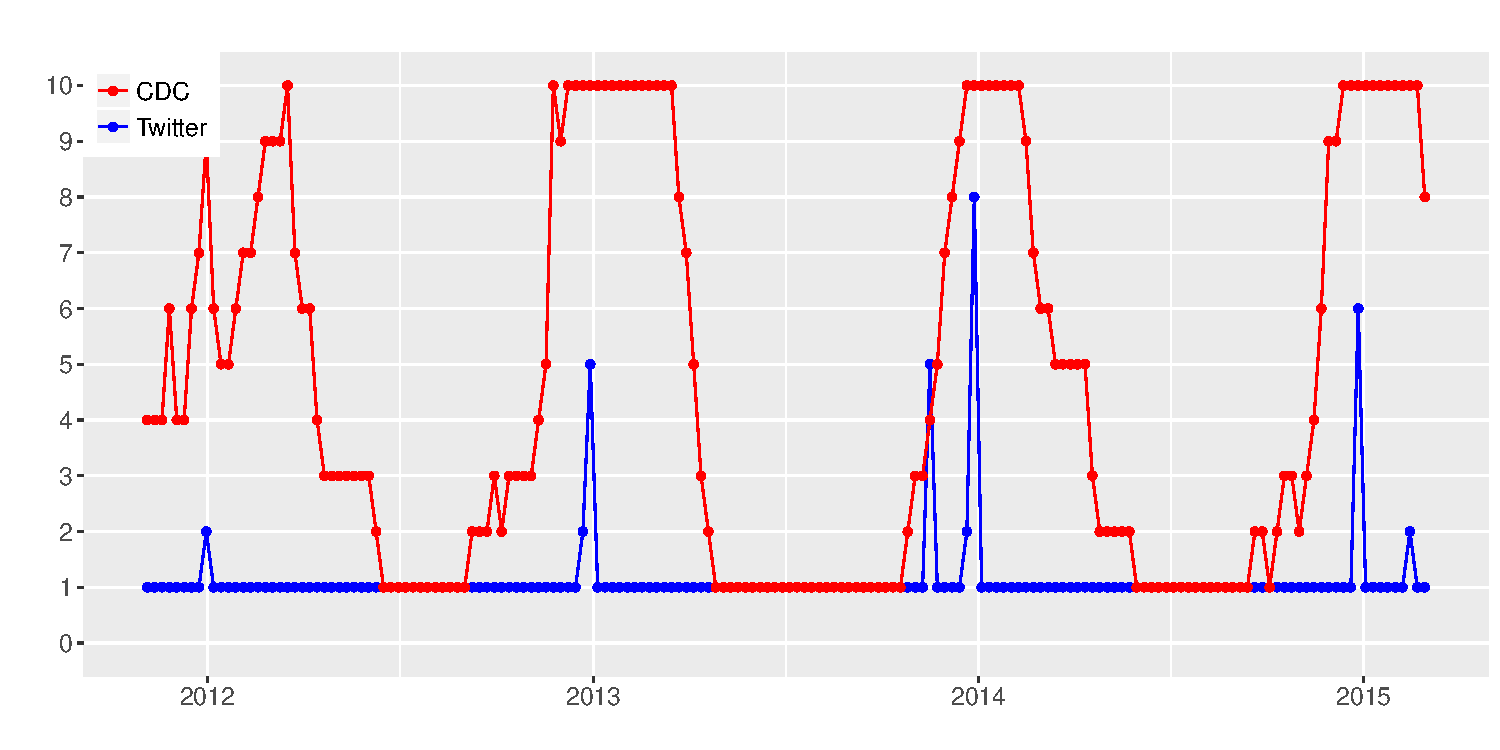
\includegraphics[width=1\linewidth]{34_cdc_twitter_comp_nat_activity_sick.pdf}
    \caption{}
  \label{fig:cdc_tw_comp_nat_ac_sick}
  \end{subfigure}
  
  \begin{subfigure}[t]{1\textwidth}
  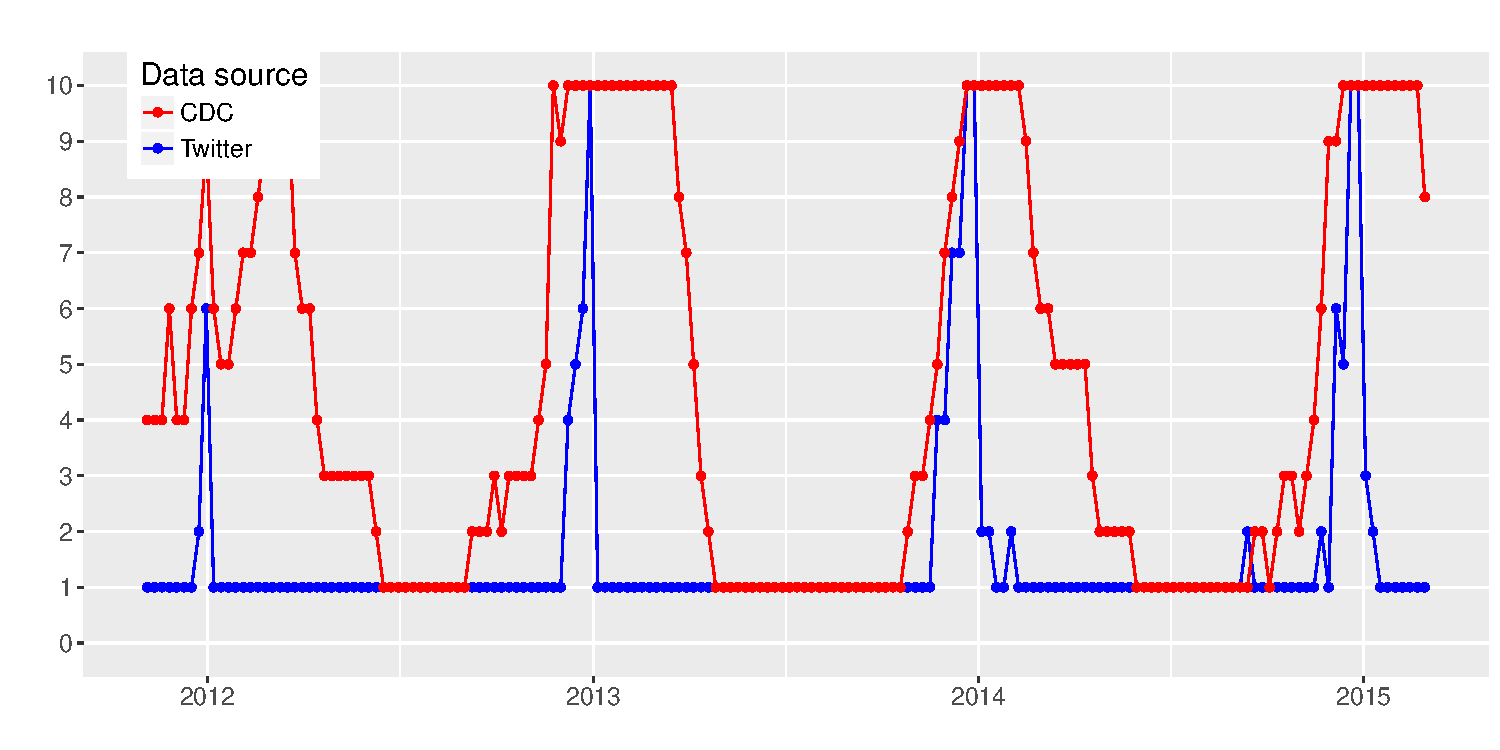
\includegraphics[width=1\linewidth]{35_cdc_twitter_comp_nat_activity_sick_user.pdf}
    \caption{}
  \label{fig:cdc_tw_comp_nat_ac_sick_user}
  \end{subfigure}
  
  \caption{Comparison between the weekly ILI activity levels reported by the CDC and the activity levels calculated based on the Twitter data set. (a) Twitter activity levels based on the relative number of sick tweets (b) Twitter activity levels calculated based on the relative number of sick users}
\end{figure}

\begin{figure}[htbp!]
\centering
  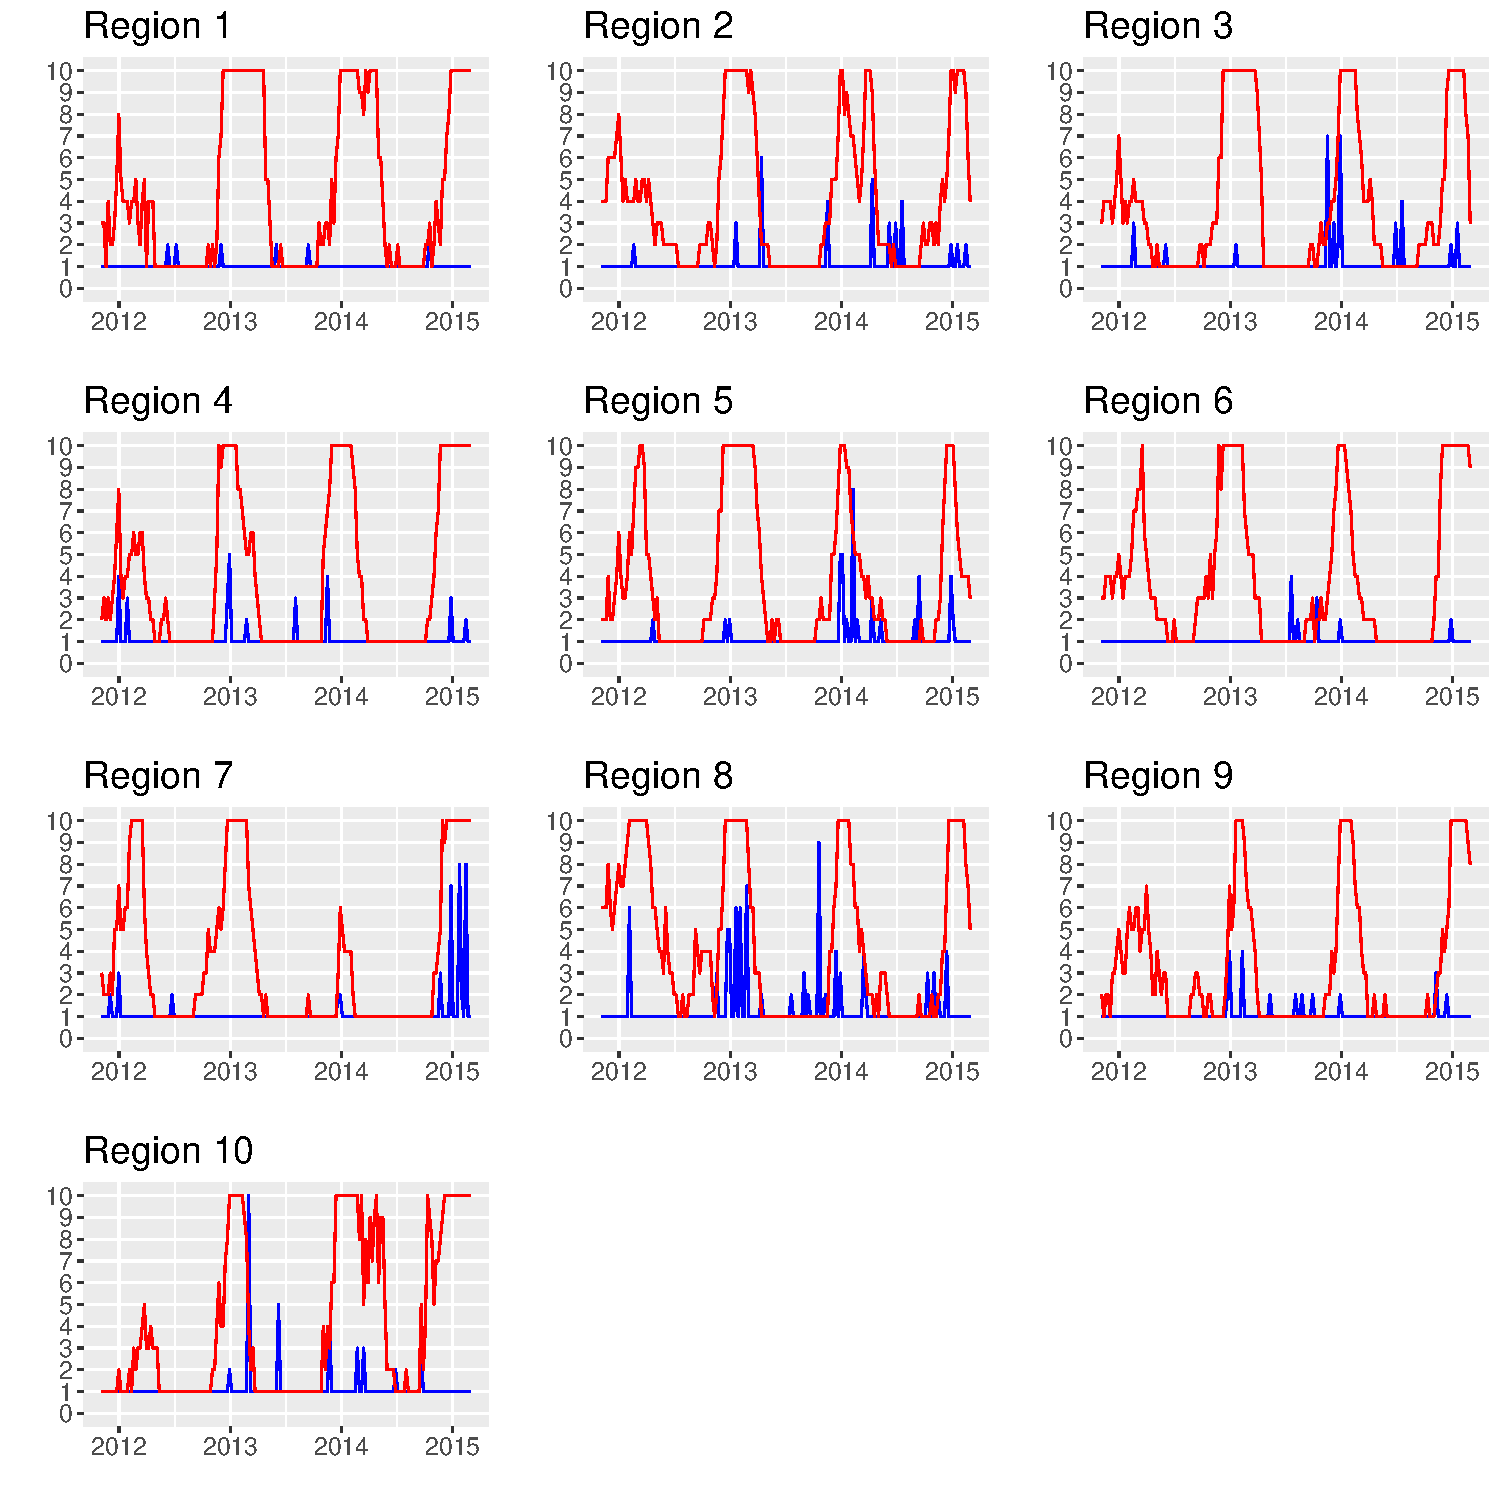
\includegraphics[width=1\linewidth]{36_cdc_twitter_comp_regs_activity_sick.pdf}
  \caption{Comparison between the regional weekly ILI activity levels reported by the CDC and the activity levels calculated based on the relative number of sick tweets per week.}
    \label{fig:cdc_tw_comp_regs_ac_sick}
\end{figure}

\begin{figure}[htbp!]
\centering
  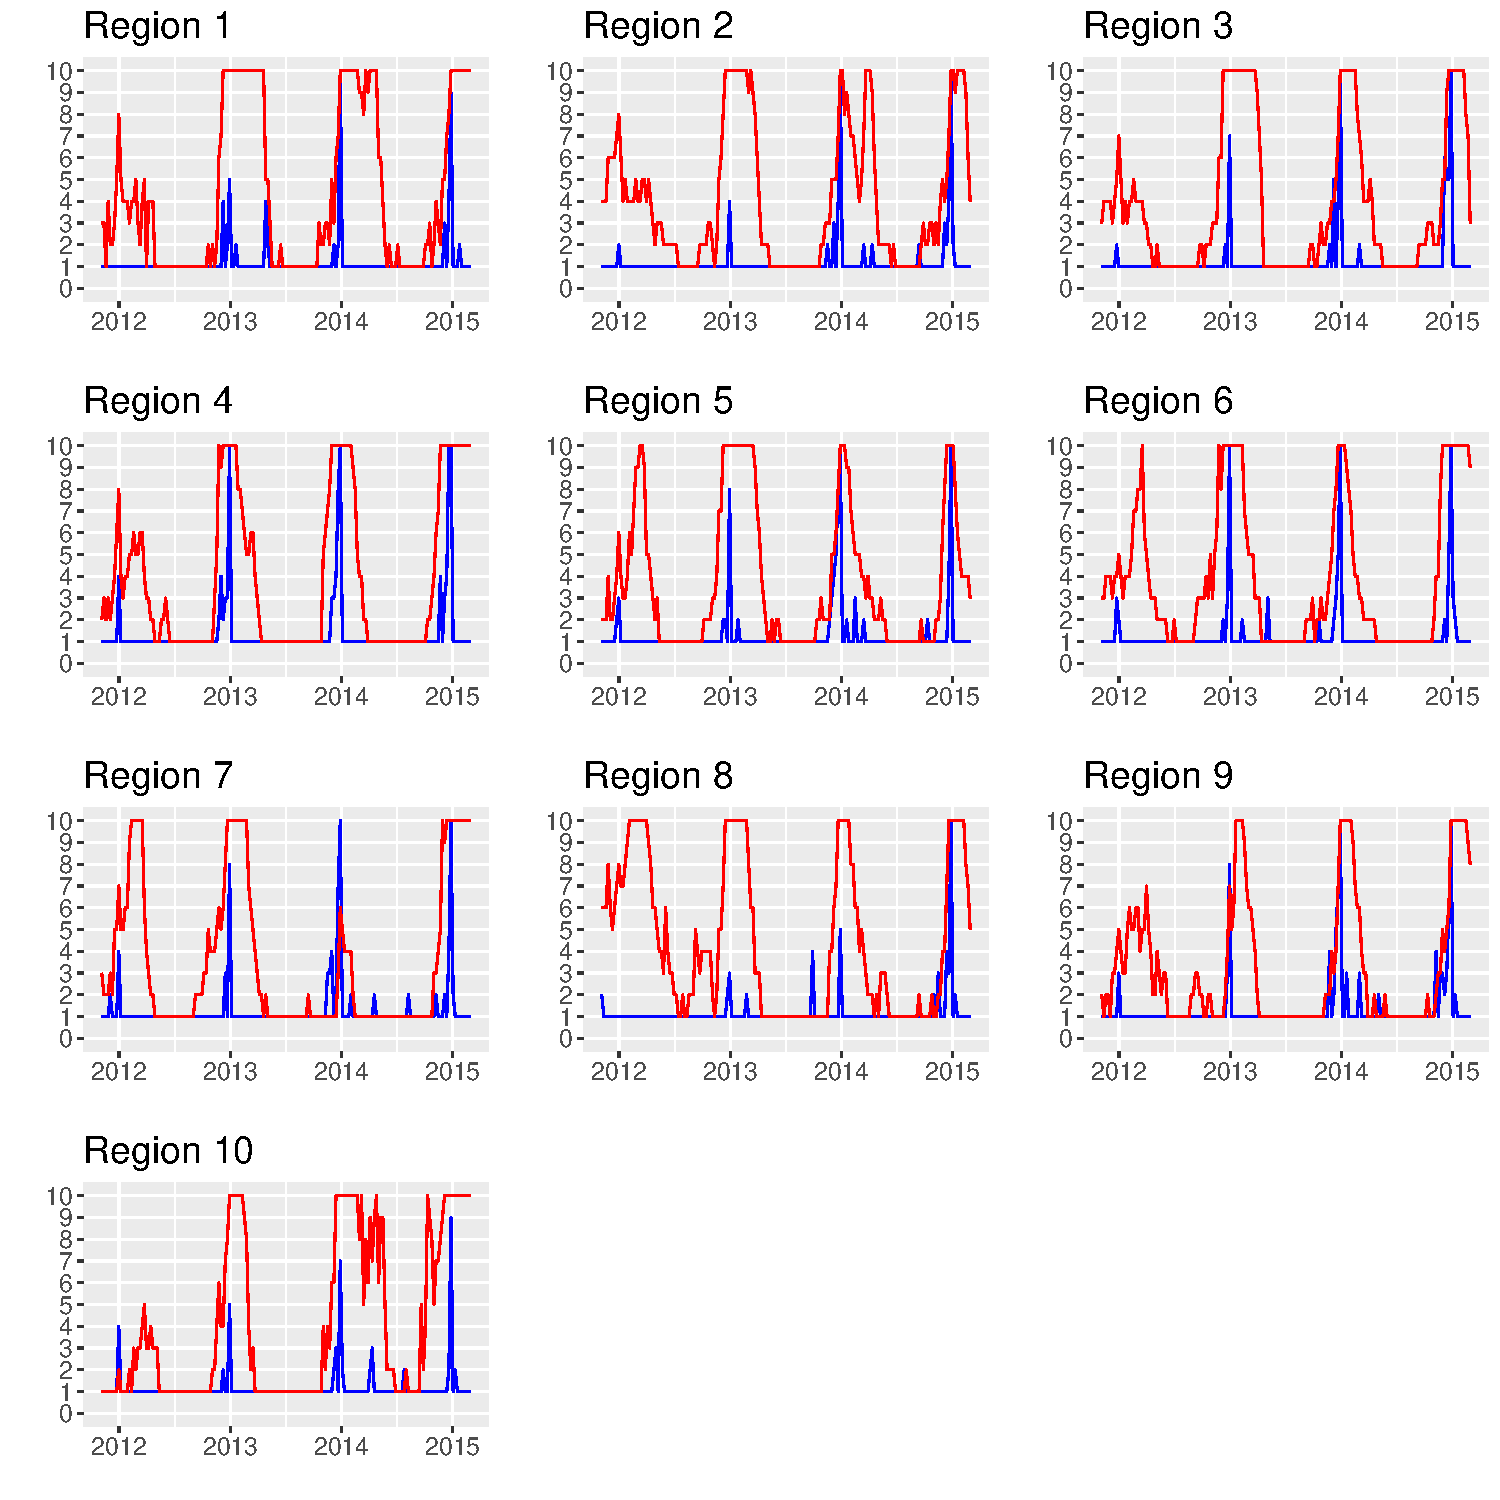
\includegraphics[width=1\linewidth]{37_cdc_twitter_comp_regs_activity_sick_user.pdf}
  \caption{Comparison between the regional weekly ILI activity levels reported by the CDC and the activity levels calculated based on the relative number of sick users per week.}
    \label{fig:cdc_tw_comp_regs_ac_sick_user}
\end{figure}\clearpage

To get a better understanding of the spatio-temporal pattern of ILI activity levels, I additionally built a function that would take CDC ILI data as well as classified Twitter data and build a map of flu activity over time. Below, you can see the two videos showing the activity levels based on the ILI rates provided by the CDC and the flu rates indicated by the Twitter classifier, respectively. Video~\ref{fig:cdc_flu_regio} contains a visualisation of the ILI activation levels provided by the CDC and serves as proof of principle for the validity of the time-lapsed flu map, allowing for a direct visualisation of the yearly flu epidemics in the USA. Video~\ref{fig:twitter_flu_regio} also shows regional activity levels, but the results from the Twitter classifier. 

\begin{center}
\href{run:vids/1_cdc_flu_regio.avi}{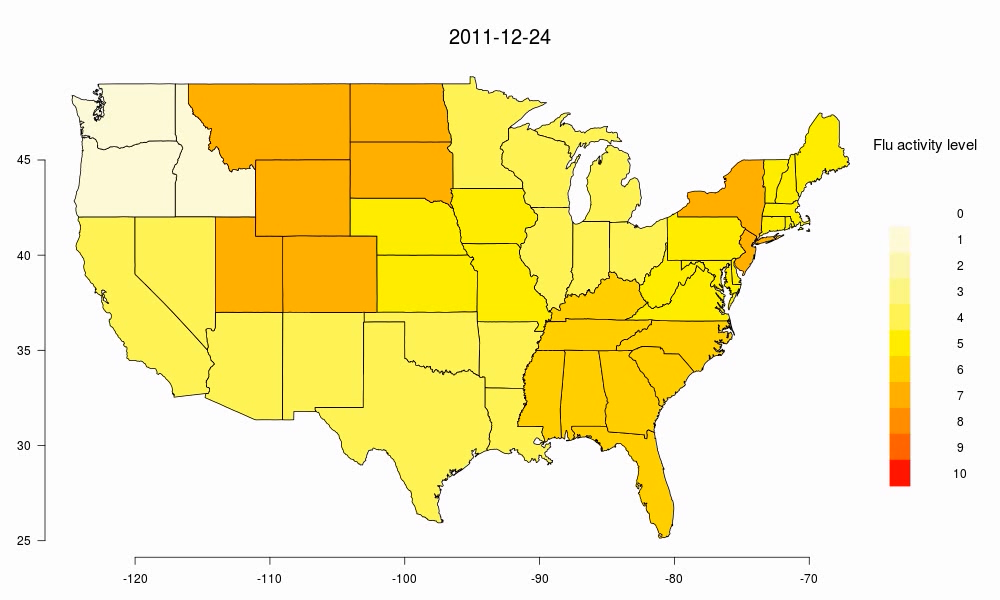
\includegraphics[width=0.9\linewidth]{vids/1_cdc_flu_regio.png}}
\end{center}
\begin{figure}[htbp!]
\centering
  \caption{ILI activity levels as provided by the CDC for the 10 surveillance regions. Red corresponds to activity level 10, while light yellow corresponds to activity level 1, which indicate the highest and lowest ILI activity, respectively. The PDF-version of this thesis contains a playable video.}
    \label{fig:cdc_flu_regio}
\end{figure}

\begin{center}
\href{run:vids/2_twitter_flu_regio.avi}{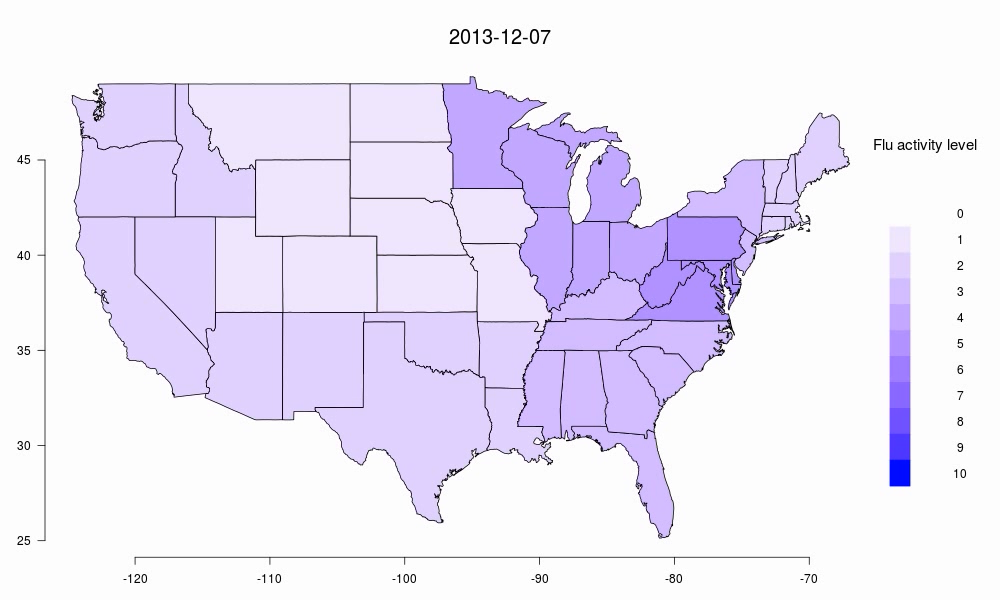
\includegraphics[width=0.9\linewidth]{vids/2_twitter_flu_regio.png}}
\end{center}
\begin{figure}[htbp!]
\centering
  \caption{Flu activity levels as calculated based on the relative number of Twitter users classified as ``sick" in each week aggregated within each of the 10 surveillance regions. Dark blue corresponds to activity level 10, while light blue corresponds to activity level 1, which indicate the highest and lowest ILI activity, respectively. The PDF-version of this thesis contains a playable video.}
    \label{fig:twitter_flu_regio}
\end{figure}

In order to directly compare the CDC and Twitter flu activity levels, I subtracted the Twitter activity levels in each week and region from each corresponding CDC activity level. I then remapped the values onto the USA over the whole 208 week interval for which I had data. Video~\ref{fig:cdc_twitter_comp_regio} shows performance of the Twitter classifier results over space and time. As can be seen, the Twitter ILI classifier hardly ever manages to emulate the CDC activity levels and when it does, it mainly happens during off-season weeks. 

\begin{center}
\href{run:vids/3_cdc_twitter_diff_user_regio.avi}{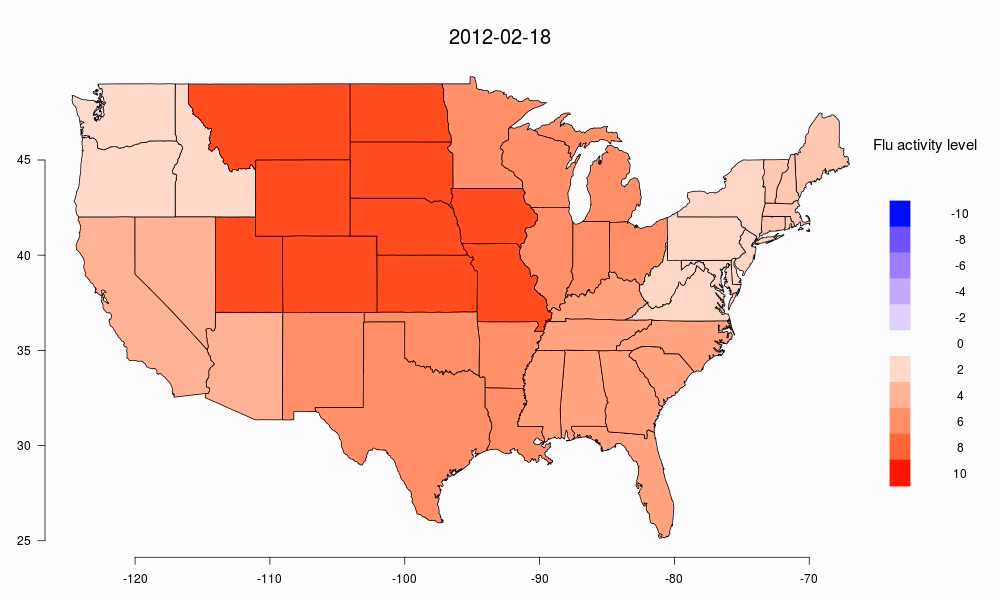
\includegraphics[width=0.9\linewidth]{vids/3_cdc_twitter_diff_user_regio.png}}
\end{center}
\begin{figure}[htbp!]
\centering
  \caption{Difference between the official ILI activity levels provided by the CDC and those calculated based on the relative amount of sick Twitter users in each corresponding region and week. White means that CDC and Twitter activity levels are exactly the same, red means that the CDC reported higher ILI activity levels in a given state and week than those calculated from the Twitter data set, blue indicates the opposite.}
    \label{fig:cdc_twitter_comp_regio}
\end{figure}

\subsection{Comparing classifier results and ILI rates on the state level}
\label{sec:comp_cdc_state}
In a next step, I tried to assess the performance of Twitter flu classifier by looking at state-level data. To do so, I again calculated activity levels for each state and week based on the relative amount of tweets labelled as ``sick" and the relative number of users classified as ``sick", respectively. Since the fit with the CDC activity curves was worse than for the regional and national data, I did not include the individual time series to this thesis, but only the a video showing the spatio-temporal differences in ILI activity levels (all additional videos and figures can be found on Github, however). Video~\ref{fig:cdc_twitter_comp_state} contains the comparison with activity levels based on the relative number of users classified as ``sick" during a specific week and within a given state. Again, it is clear the activity levels based on the Twitter data fit the official CDC only poorly.

\begin{center}
\href{run:vids/4_cdc_twitter_diff_user_state.avi}{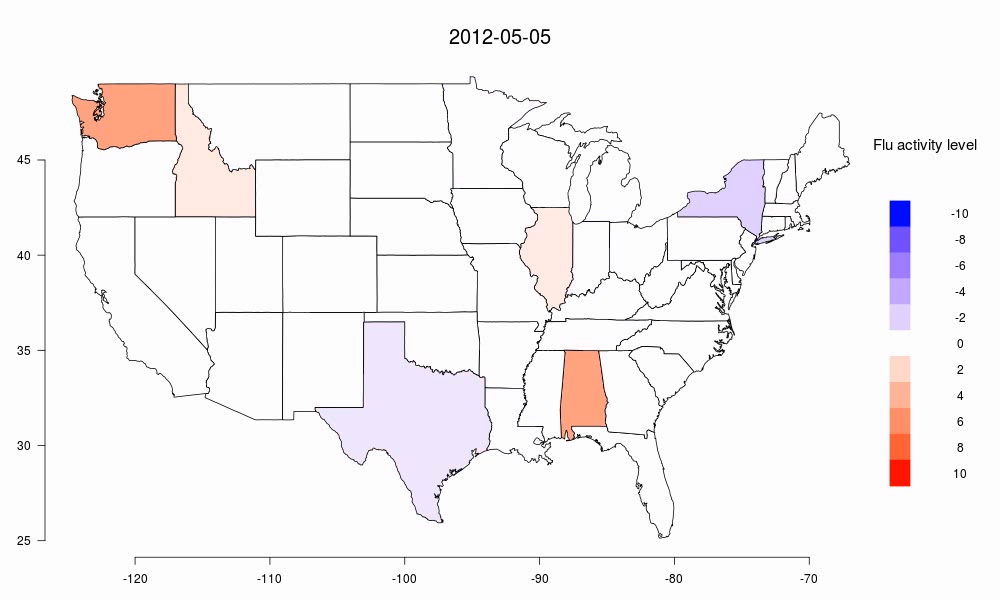
\includegraphics[width=0.9\linewidth]{vids/4_cdc_twitter_diff_user_state.png}}
\end{center}
\begin{figure}[htbp!]
\centering
  \caption{Difference between the official ILI activity levels provided by the CDC and those calculated based on the relative amount of sick Twitter users in each corresponding state and week. White means that CDC and Twitter activity levels are exactly the same, red means that the CDC reported higher ILI activity levels in a given state and week than those calculated from the Twitter data set, blue indicates the opposite.}
    \label{fig:cdc_twitter_comp_state}
\end{figure}

\subsection{Comparing classifier results and ILI rates on the county level}
\label{sec:comp_cdc_county}
In order to assess the performance of the classifier on the county level, I contacted 18 state health departments (Arkansas, California, Florida, Illinois, Iowa, Louisiana, Maine, Michigan, Minnesota, Mississippi, Missouri, New Jersey, New York, North Dakota, Oregon, South Dakota), asking them for their county-level or regional ILI data between 2011 and 2015. I only received the county-level data from the state of Oregon, while the state of California provided me with state-level data only. All other states did either not answer or declined my request. Luckily, the states of New Jersey and Mississippi provided (almost) complete county-level ILI data on their website for the requested time period. Since the data was only provided in PDF-format, I built a scraper for both states in order to retrieve the relevant information. 

Below, you can see the spatio-temporal comparison of the performance of the Twitter flu classifier for the counties of New Jersey (Video~\ref{fig:cdc_twitter_comp_jersey}) and Oregon (Video~\ref{fig:cdc_twitter_comp_oregon}). Note, that Oregon did not provide ILI estimates for all counties (most of the northeastern counties are missing, for example).

\begin{center}
\href{run:vids/5_cdc_twitter_diff_user_jersey.avi}{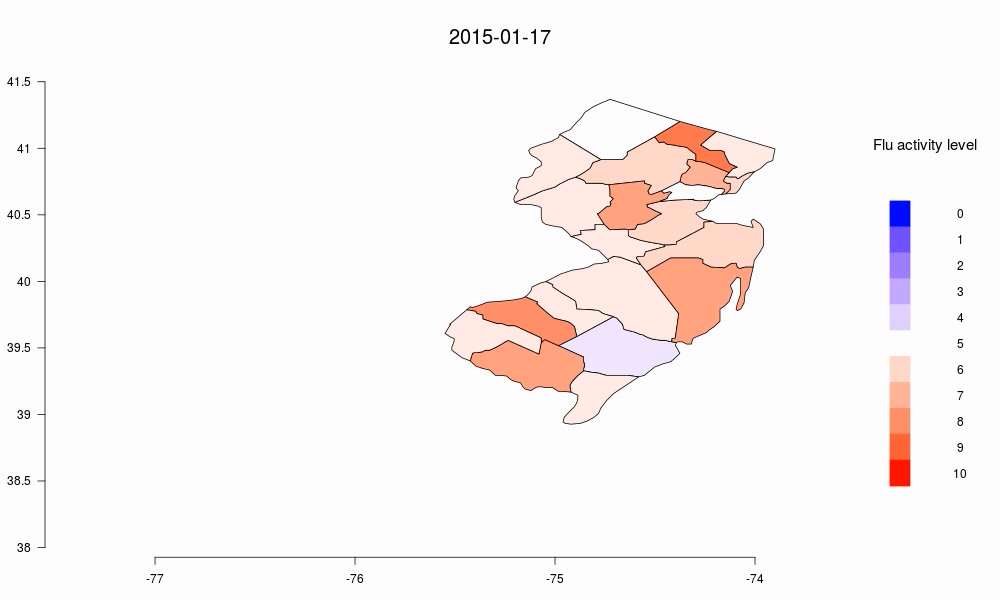
\includegraphics[width=0.9\linewidth]{vids/5_cdc_twitter_diff_user_jersey.png}}
\end{center}
\begin{figure}[htbp!]
\centering
  \caption{Difference between the official ILI activity levels provided by the state of New Jersey and those calculated based on the relative amount of sick Twitter users in each corresponding week and county of New Jersey. White means that the official and Twitter activity levels are exactly the same, red means that the state of New Jersey reported higher ILI activity levels in a given county and week than those calculated from the Twitter data set, blue indicates the opposite.}
    \label{fig:cdc_twitter_comp_jersey}
\end{figure}

\begin{center}
\href{run:vids/6_cdc_twitter_diff_user_oregon.avi}{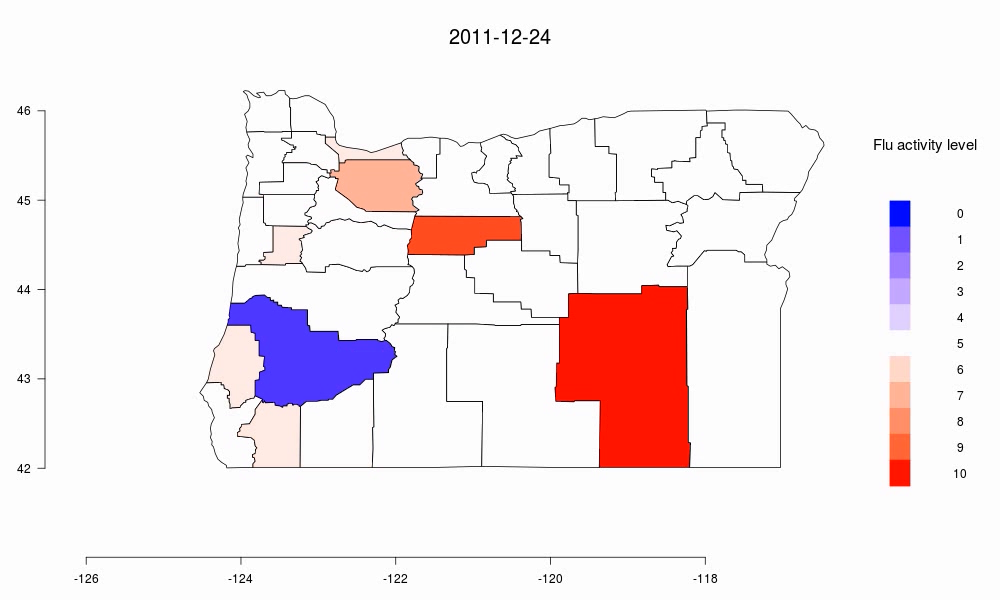
\includegraphics[width=0.9\linewidth]{vids/6_cdc_twitter_diff_user_oregon.png}}
\end{center}
\begin{figure}[htbp!]
\centering
  \caption{Difference between the official ILI activity levels provided by the state of New Jersey and those calculated based on the relative amount of sick Twitter users in each corresponding week and county of Oregon. White means that the official and Twitter activity levels are exactly the same, red means that the state of Oregon reported higher ILI activity levels in a given county and week than those calculated from the Twitter data set, blue indicates the opposite.}
    \label{fig:cdc_twitter_comp_oregon}
\end{figure}

\section{Attempts to reproduce key figures and findings from \cite{bodnar_data_2015}}
\label{sec:methods_reproduce}
As the results depicted above show, the output from the Twitter classifier that served as the basis of my analysis does neither serve as a very good approximation of the official CDC data nor does it reflect the results shown in \cite{bodnar_data_2015}. There are various potential reasons for this which I will lay out in Chapter~\ref{ch:discussion}. Before doing so, however, I will summarise additional attempts of mine to reproduce some key results reported in \cite{bodnar_data_2015}.

\subsection{Reclassification of the raw Twitter data}
As described in Chapter~\ref{ch:data_set_description}, the data set I was working with a data set that contained the output of the Twitter classifier described in Chapter~\ref{ch:intro}. Since there might very well be discrepancies between this data set and the one used in \citep{bodnar_data_2015}, I wanted to reclassify the geotagged raw Twitter data collected between 2011 and 2015 in order to assess whether these results would diverge from the data set I was working on.

To do so, I retrieved the full Java-based Twitter classifier from Todd Bodnar's \href{https://github.com/ToddBodnar/Twitter-Parser}{Github repository}. However, some libraries used for building the classifier were missing from the repository, while others (most notably the \href{https://aws.amazon.com/de/sdk-for-java/}{Amazon Web Services (AWS) SDK for Java} have in the meantime been superceded by newer vesions which are not backwards compatible with older version and thus incompatible with the Twitter classifier. Even though I managed to retrieve the missing libraries through personal communication with Todd Bodnar and also managed to retrieve the same AWS SDK version that was used for the original version of the Twitter classifier, additional compilation errors remained, so I was unable to compile the classifier.

Finally, I received a compiled version of the Twitter classifier (``TwitterParser.jar") directly from Todd Bodnar, allowing me to circumvent the necessity to debug the original code.  Unfortunately, the jar-file encountered runtime erros when trying to analyse raw Twitter files, both on Ubuntu 16.04.2 LTS as well as on Windows 7. Hence, I still failed to reclassify the raw Twitter data using the Twitter classifier. All files belonging to the Twitter classifier, including the compiled version of it, can be found on \href{https://github.com/salathegroup/2016_TwitterEpi}{Github} in the folder ``Twitter\_Parser".

\subsection{Reproduction of the SIR model described in \cite{bodnar_data_2015}}
Since I was unable to reproduce the original results of the Twitter classifier due to compilation and runtime errors of said classifier, and hence was unable to assess the validiy of the data set I was working on, I went at it from the opposite direction: I started from the final results described in \cite{bodnar_data_2015} and tried to ``reverse engineer" them in order to learn how the excellent fit of the Twitter data with the CDC data came about. Specifically, I focused on chapter 4 of \cite{bodnar_data_2015} and tried to reproduce the findings shown in Figures~\ref{fig:cdc_fit_bodnar_thesis} and \ref{fig:cdc_fit_bodnar_thesis_SIR} as well as Table~\ref{tab:nationalparams}.

In a first step, I asked Todd Bodnar for the data and the code used to create the SIR model as well as the figures. I received the R-files used to build the SIR model as well csv-files containing the data used to create Figures~\ref{fig:cdc_fit_bodnar_thesis} and \ref{fig:cdc_fit_bodnar_thesis_SIR}  However, I did not receive the R-files or the model specifications in order to create the data contained in said file from the Twitter data set. Hence, I could neither associate the data within these files to the raw results from the Twitter classifier nor to the R-code-files that were provided to me. A follow-up e-mail regarding this matter is pending response. Data and code files can be found on \href{https://github.com/salathegroup/2016_TwitterEpi}{Github} in the folder ``PhDThesisBodnar".

In order to recreate the figures mentioned above, I used the data available in the file ``predictions\_r\_results.csv", which contained weekly ILI estimates from the CDC as well as additional ILI estimates using different autocorrelation models with or without using the data from the Twitter classifier. The data spanned a four year period, starting on October $3^{rd}$ 2011 (week 40) and ending on September $28^{th}$ 2014 (week 39). The 11 columns contained in the data set have the following meaning (Bodnar, personal communication):

\begin{itemize}
  \item \texttt{cdcoffset} The official ILI data from the CDC
  \item \texttt{predictions\_base} The percentage of Twitter users classified as ill based on the predictive base model
  \item \texttt{predictions\_autocor} Predictive AR(1) model based on the ``cdcoffset" data
  \item \texttt{predictions\_autocor2} Predictive AR(2) model based on the ``cdcoffset" data
  \item \texttt{predictions\_both} Predictive AR(1) model based on the ``cdcoffset" data combined with the values from the predictive Twitter base model
  \item \texttt{predictions\_both2} Predictive AR(2) model based on the ``cdcoffset" data combined with the values from the predictive Twitter base model
 \item \texttt{full\_base} The percentage of Twitter users classified as ill based on the retrospective base model
  \item \texttt{full\_autocor} Retrospective AR(1) model based on the ``cdcoffset" data
  \item \texttt{full\_autocor2} Retrospective AR(2) model based on the ``cdcoffset" data
  \item \texttt{full\_both} Retrospective AR(1) model based on the ``cdcoffset" data combined with the values from the retrospective Twitter base model
  \item \texttt{full\_both2} Retrospective AR(2) model based on the ``cdcoffset" data combined with the values from the retrospective Twitter base model
\end{itemize}

For the predictive models, only values between weeks $0$ and $t-1$ were used for model building, for the retrospective models the complete available data was used. According to Bodnar \texttt{full\_base} column corresponds to the weekly aggregated results of the Twitter classifier (personal communication).

I started with the replication of Figure~\ref{fig:cdc_fit_bodnar_thesis_SIR} and the corresponding parameters. I did so by using the grid-search method described in \cite{bodnar_data_2015}: 

``Specifically, we search through three variables, the two transmission parameters $\gamma$,$\beta$, and S(0), the initial susceptibility rate which may be less than 1 due to innate immunity or previous vaccination. Next, we generate a logarithmically spaced 25 by 25 by 25 grid of potential values over this range. We then set $I(0)$ to be the same as the first infection value in the data and $R(0)$ (sic!). We then solve an SIR model, with each of the parameter combinations." 

Note that in the R-code I received the optimisation only happened for $\gamma$ and $\beta$, not for $S(0)$, as desribed. This makes intuitive sense: Since we know the initial value of $I(0)$ both for the CDC data as well as for the Twitter model, there is no need to algorithmically find the initial value of $S(0)$, since it can simply be calculated as $S(0)=1-I(0)$, while $R(0)=0$. Indeed, this is exactly the way the initial values were set in the algorithm.

First, I built the SIR model based on the CDC data, since this was the most straightforward way to go. As can be seen from Figure~\ref{fig:SIR_comparison_CDC}, the yearly and combined ILI curves calculated from the model are very similar to the ones depicted in Figure~\ref{fig:cdc_fit_bodnar_thesis_SIR}, however small deviations remain.

Therefore, I went on to fit the very same SIR model that is shown in Figure~\ref{fig:cdc_fit_bodnar_thesis_SIR}. To do so, I needed to know which data the model was built on. I extracted the three starting coordinates of the yearly curves shown in the figure and compared them with the data provided to me by Todd. It turned out that the starting coordinates of the curve only matched the values from the full retrospective Twitter model (i.e. retrospective AR(2) model based on the CDC data combined with the retrospective Twitter base model), so I built my second SIR model based on these values. As can be seen from Figure~\ref{fig:SIR_comparison_full}, the resulting yearly and combined ILI curves are virtually indistinguishable from the ones shown in \cite{bodnar_data_2015}.

It is very peculiar, however, that the model parameters which I calculated for the two replicated SIR models described above do not match the yearly and combined values for $\gamma$ and $\beta$ presented in \citep{bodnar_data_2015}---even though the model curves seem to match. As can be seen from Table~\ref{tab:nationalparams_replicated}, the optimal yearly and combined values of $\gamma$ and $\beta$ deviate considerably from the ones depicted in Table~\ref{tab:nationalparams} (i.e. the values reported in \citep{bodnar_data_2015}). This is true for the SIR model based on the CDC data as well as for the SIR model based on the full retrospective model data. At the same time, however, the curves that result when creating an SIR model based on the values in Table~\ref{tab:nationalparams_replicated} and the \texttt{full\_both2} data provided to me are virtually indistinguishable from the curves depicted in \cite{bodnar_data_2015}, i.e. in Figure~\ref{fig:cdc_fit_bodnar_thesis_SIR}. This implies that the $\beta$ and $\gamma$ values reported in \cite{bodnar_data_2015} are not the ones that were used to create Figure~\ref{fig:cdc_fit_bodnar_thesis_SIR}.

In order to corroborate this assumption, I recreated SIR model curves based on the values reported in Table~\ref{tab:nationalparams} and compared them to the SIR model curves resulting from the values in Table~\ref{tab:nationalparams_replicated}, which are depicted in cyan and blue, respectively, in Figure~\ref{fig:40A_40B_remodeling_comparison}. The comparison reveals a marked difference between the two model curves and makes clear that the model curves based on the recreated values in Table~\ref{tab:nationalparams_replicated} are much more similar to the original curves depicted in in Figure~\ref{fig:cdc_fit_bodnar_thesis_SIR} than the model curves based on the values from \cite{bodnar_data_2015} depicted in Table~\ref{tab:nationalparams}.

 \begin{table}[htbp!]
\centering
\caption{Combined and yearly best-fit parameters for the SIR model I recalculated based on the CDC's data (white) and the Twitter base model data (grey) provided to me by Bodnar (personal communication).}
\begin{tabular}{l l l l l}
 Year & \(\gamma\) & \(\beta\) & RSS\\ \hline
& 0.3962286 & 0.4446748  & \ensuremath{4.0608281\times 10^{-4}}   \\ 
 {\multirow{-2}{*}{ 2011-2012 }}  & \cellcolor{grey}0.3666311  & \cellcolor{grey}0.4087479 & \cellcolor{grey}\ensuremath{3.6266689\times 10^{-4}}  \\ \cline{2-4}
  {\multirow{2}{*}{ 2012-2013 }}& 0.5121045 & 0.6777425  & 0.0029532  \\ 
   & \cellcolor{grey}0.5021989  & \cellcolor{grey}0.6546756 & \cellcolor{grey}0.0027735   \\ \cline{2-4}
  {\multirow{2}{*}{ 2013-2014 }}& 0.451297 & 0.5699723    & 0.0014841   \\ 
   & \cellcolor{grey}0.4294719 & \cellcolor{grey}0.535259 & \cellcolor{grey}0.0013076  \\ \cline{2-4}
  {\multirow{2}{*}{ Combined }}& 0.4878438 & 0.6068527 & 0.008631   \\ 
   & \cellcolor{grey}0.4641424  & \cellcolor{grey}0.5698395  & \cellcolor{grey}0.0077089   \\ 
\end{tabular}
\label{tab:nationalparams_replicated}
\end{table}

\begin{figure}[htbp!]
\centering
  \begin{subfigure}[t]{1\textwidth}
  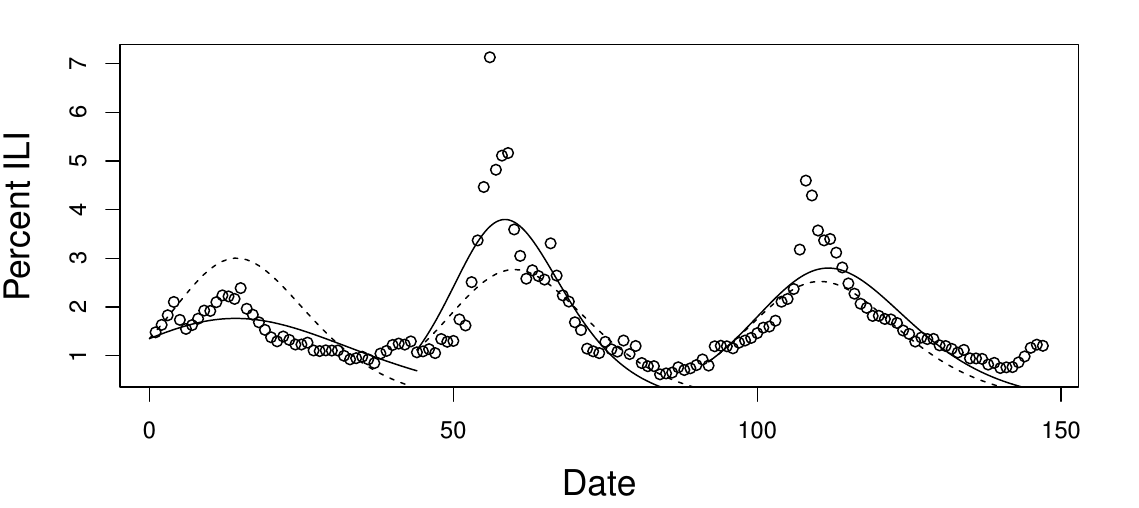
\includegraphics[width=1\linewidth]{02_todd_bodnar_SIR.png}
  \caption{}
  \end{subfigure}
  
  \begin{subfigure}[t]{1\textwidth}
  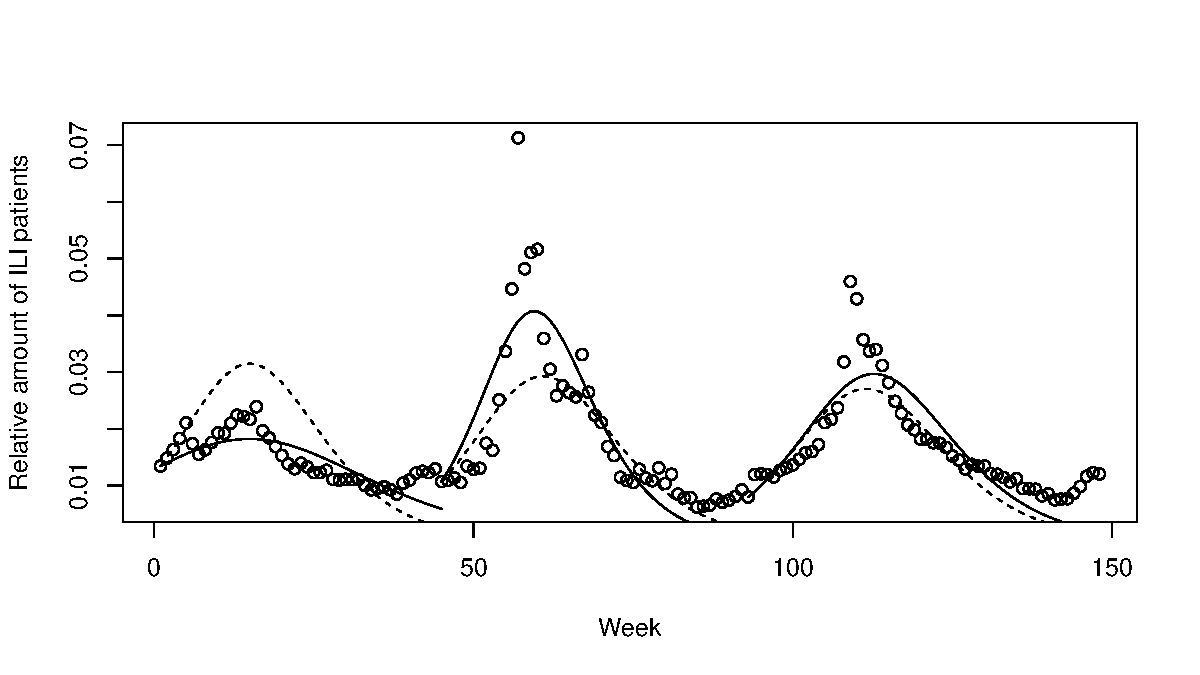
\includegraphics[width=1\linewidth]{38_SIR_model_cdc_data_25.pdf}
  \caption{}
  \end{subfigure}
  \caption{Comparison between the SIR model depicted in \cite{bodnar_data_2015} (a) and a replication based on the official CDC ILI rates (b).}
  \label{fig:SIR_comparison_CDC}
  %\label{fig:SIR_comparison}
\end{figure}

\begin{figure}[htbp!]
\centering
  \begin{subfigure}[t]{1\textwidth}
  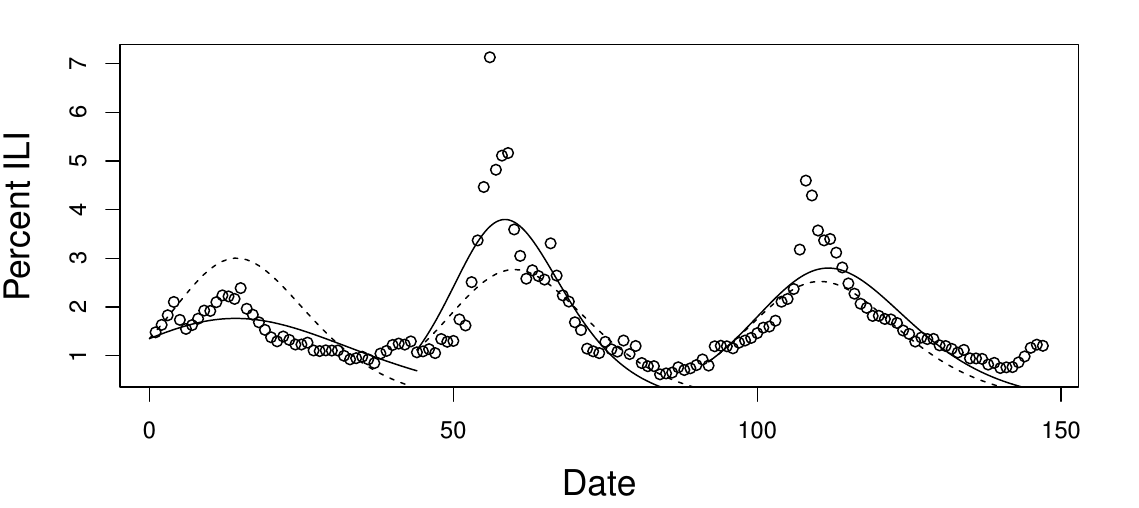
\includegraphics[width=1\linewidth]{02_todd_bodnar_SIR.png}
  \caption{}
  \label{fig:SIR_comparison_original}
  \end{subfigure}

  \begin{subfigure}[t]{1\textwidth}
  \includegraphics[width=1\linewidth]{39_SIR_model_full_model_25.pdf}
  \caption{}
  \label{fig:SIR_comparison_full}
  \end{subfigure}
  \caption{Comparison between the SIR model depicted in \citep{bodnar_data_2015} (a) and a replication based on the full retrospective Twitter model (c).}
    \label{fig:SIR_comparison_CDC_full_model}
\end{figure}

\begin{figure}[htbp!]
\centering
  \begin{subfigure}[t]{1\textwidth}
  \includegraphics[width=1\linewidth]{40A_SIR_model_full_model_25_comparison_yearly.pdf}
  \caption{}
  \end{subfigure}
  
  \begin{subfigure}[t]{1\textwidth}
  \includegraphics[width=1\linewidth]{40B_SIR_model_full_model_25_comparison_combined.pdf}
  \caption{}
  \end{subfigure}
  \caption{SIR model curves using yearly (a) and combined (b) paramaters to model the ILI prevalence throughout one year. Red indicates the official ILI rates from the CDC, while cyan and blue show the SIR model curves based on the parameters reported in \cite{bodnar_data_2015} and the ones recalculated by me, respectively, based on the very same data (i.e. the \texttt{full\_both2} values).}
  \label{fig:40A_40B_remodeling_comparison}
  %\label{fig:SIR_comparison}
\end{figure}

\subsection{Attempt to reproduce the AR model described in \cite{bodnar_data_2015}}
It is important to note once again that the data used to calculate the SIR models in \cite{bodnar_data_2015} are \textit{not} equivalent the \texttt{full\_base} data, which are supposed to represent the raw output from the Twitter classifier according to Bodnar (personal communication). In fact, the SIR models described above are built on the full retrospective model data which includes the information from the Twitter classifier as well as information from an AR(2) model based on the official CDC data. This stands in contrast to the report in \cite{bodnar_data_2015}, where the SIR models are depicted as being based on the information from the Twitter classifier only. However, as I have shown in the previous section, this cannot be the case and it is neither the case for the results shown in Figure~\ref{fig:cdc_fit_bodnar_thesis}.

The graph is described as the ``comparison of Twitter's forecasting (dashed lines) and retroactive measurements (solid lines) to the CDC's reported Influenza rates (circles)", therefory implying that the dashed and solid lines are produced based on the data from the Twitter classifier alone. However, this is clearly not the case. Figure~\ref{fig:TwitterModel_original} shows a reproduction of the original graph depicted in \citep{bodnar_data_2015}, including SIR model fits. However, this reproduction is based on the retrospective \textit{full} model, i.e. the model corresponding to the \texttt{full\_both2} data and including information from the Twitter base model as well as from the AR(2) model based on the CDC data. If we only look at the data from the Twitter base model (Figure~\ref{fig:TwitterModel_comparison_base}), we can see that the fit with the official CDC data is worse and that the corresponding SIR model is also decidedly different from the SIR model based on the \texttt{full\_both2} values. Also, Figure~\ref{fig:TwitterModel_comparison_ar} shows that a simple AR(2) model based on the official CDC data achieves a model fit that is almost as good as the one from the full model which includes additional information from the Twitter base model.

\begin{figure}[htbp!]
\centering
  \begin{subfigure}[t]{1\textwidth}
  \includegraphics[width=1\linewidth]{40_SIR_model_full_both_25_colorised.pdf}
  \caption{}
  \label{fig:TwitterModel_original}
  \end{subfigure}
  
  \begin{subfigure}[t]{1\textwidth}
  \includegraphics[width=1\linewidth]{41_SIR_model_full_AR2_25_colorised.pdf}
  \caption{}
  \end{subfigure}
  \caption{Comparison between the full retrospective Twitter model depicted in \cite{bodnar_data_2015} (a) and a replication consisting of a simple retrospective AR(2) model based only on CDC ILI rates (b). The black lines indicate the results of the corresponding SIR models using yearly (solid) and combined (yearly) parameters.}
  \label{fig:TwitterModel_comparison_ar}
\end{figure}

\begin{figure}[htbp!]
\centering
  \begin{subfigure}[t]{1\textwidth}
  \includegraphics[width=1\linewidth]{40_SIR_model_full_both_25_colorised.pdf}
  \caption{}
  \end{subfigure}
  
  \begin{subfigure}[t]{1\textwidth}
  \includegraphics[width=1\linewidth]{42_SIR_model_full_base_model_50_colorised.pdf}
  \caption{}
  \end{subfigure}
  \caption{Comparison between the full retrospective Twitter model depicted in \cite{bodnar_data_2015} (a) and a replication consisting of the retrospective Twitter base model (b). The black lines indicate the results of the corresponding best-fit SIR models using yearly (solid) and combined (yearly) parameters.}
  \label{fig:TwitterModel_comparison_base}
\end{figure}

\thispagestyle{empty}
\cleardoublepage

\chapter{Discussion and outlook}
\label{ch:discussion}

In this last chapter, I will first discuss the findings summarised in Chapters~\ref{ch:data_set_description} and~\ref{ch:results} with a special emphasis on potential future applications of the Twitter classifier or related methods for flu surveillance.

In a second part, I will then put emphasis on the discussion of the different issues of reproducibiliy that I have outlined in Chapter~\ref{ch:reproducibility} and that have arisen during the course of this work. I will also make suggestions about how to overcome such issues in the future. 

\section{Has ``Larry the Bird" deserved our trust?}
\label{sec:disc_data_set}

The results of my comparison of the results of the Twitter classifier with the official ILI data from the CDC are mixed. The following sections will discuss the reliability of the classifier on different levels and make suggestions on how to make improvements in the future.

\subsection{The Twitter classifier can detect seasonal flu peaks on a national level}
The classifier has shown that it can faithfully predict the Influenza peaks recurring on a national level every year between the months of December and February (see Figures~\ref{fig:naive_comparison_CDC_twitter}, \ref{fig:cdc_tw_comp_nat_tot}, and \ref{fig:cdc_tw_comp_nat_user}). 

However, one can also see from these figures that the peaks are very short and sharp. This might be explained by the way the Twitter classifier labels a certain tweet---and thereby its author---as ``sick". The classifier does so by aggregating the daily signals within a 4-week-window in order to classify the tweets of the first day either as ``sick" or ``healthy" (see Section~\ref{sec:on_the_ground} for details). 

But this way of assigning disease status has one problematic implication, namely that information from future tweets is incorporated while information from past tweets is ignored. This is insofar counterintuitive as a Twitter user who tweeted about being sick on day 1, will most certainly still be sick on day 2---regardless of what he tweets about. However, the algorithm will not take this into account, so when shifting the onset of the 4-week-sliding window to day 2, all information from day 1 will be lost. If there are no additional flu keywords to be found in the tweets sent within the following 4-week-sliding window, the algorithm will mistakenly classify the user as being healthy again.

In addition, the algorithm is bound to classify tweets too early as being sick. For example, if particularly strong ``flu" signal turns appears, the algorithm might classify the user as being ``sick" up to four weeks before the actual onset of the sickness. In other words; instead of assuming that a user remains sick for some time after she has tweeted about being sick, the algorithm might give the faulty impression that the user has been sick up to the point where she tweeted about it---but not afterwards.

Of course, one can argue that a Twitter user does not necessarily tweet about her flu symptoms on the first day of the onset of the symptoms so that the exact start of the disease is difficult to assess in any case. This is true, but as long as we do not have any additional information about the probability distribution of when the user tweets about her sickness, it would be prudent to assume a uniform distribution and treat each day of the disease as having equal probability of being a day during which the user tweets about her disease. 

In any case, the fact that the classifier assigns disease status only on the first day of the 4-week-sliding window and only by taking into account prospective information, might artificially shorten the duration in which a user is classified as having the flu. On a population level, this might lead to the sharp and short peaks we can observe in the figures referenced above. Future revisions of the Twitter classifier should therefore also take into consideration retrospective information from a Twitter user's timeline and not classify the tweets of the first day of the 4-week-sliding window, but the tweets of the 14th or 15th day, i.e. a day in the middle of said window.

\subsection{The Twitter classifier might be able to detect ILI symptoms in summer}
Another peculiar finding from the comparison of CDC and Twitter classifier data is the overestimation of ILI symptoms in summer by the classifer. This can clearly be seen in Figures~\ref{fig:naive_comparison_CDC_twitter}, \ref{fig:cdc_tw_comp_nat_tot}, and \ref{fig:cdc_tw_comp_nat_user} as well as in Video~\ref{fig:twitter_flu_regio} and is most prominent in the summer of 2011. 

Since the classifier was built using confirmed medical records that could be correlated on an individual basis with the output of specific Twitter users, it is very unlikely that the peaks in summer are due to overfitting, especially because the set of users on which the classifier was validated was very small. 

However, as outlined in Section~\ref{sec:on_the_ground}, the small sample size that served to build the classifier in combination with its low temporal resolution could have introduced other biases which might jeopardise the generalisability of the classifier up to the point at which it is useless outside the very specific enviroment in which it was built (the Pennsylvania State University and part of its student body in the year 2011--2012). However, if that were the case, we would expect the classifier to fail to detect the flu peaks in winter, for example. Since this is not the case, however, we can safely assume that rules which the classifier uses to detect flu-related tweets can be applied on national level data as well. 

Hence, the most likely explanation for the peaks in summer might also be the most promising: If we can assume that the classifier is able to pick up ILI symptoms with some reliability, then we should expect the classifier to detect these signals regardless of whether the Twitter user has the flu or another disease that symptomatically resembles the flu. This is true for common colds, which lead to symptoms such as sore throat, runny nose, coughing, sneezing, headaches, and body aches, and whose occurrence coincide with that of the flu, but which are most often caused by rhinoviruses \citep{heikkinen2003common,cdc_rhinovirus_2017}. 

However, there are also many cold viruses that predominantly spread during the summer, the non-polio enteroviruses being the most notorious representative  \citep{pons2015epidemiology}. An infected person can exhibit symptoms akin to those of the flu, such as fever, runny noze, sneezing, coughing, body and muscle aches \citep{pons2015epidemiology,cdc_enterovirus_2016}.

Hence, the off-season peaks of the Twitter classifier in 2011, 2012, 2013, and 2014 could be caused by other infectious diseases that exhibit similar symptoms to that of the flu. Further assessments of the validity of the flu classifier should take this into account, for example by comparing its performance with the surveillance data of other infectious disease capable of causing ILI symptoms.

\subsection{Autoregression trumps Twitter data}
As \cite{paul_twitter_2014} noted, autoregressive models are very strong baseline models to forecast ILI prevalence---better than only using Twitter for this task. This can also be observed in Figures~\ref{fig:TwitterModel_comparison_base} and \ref{fig:TwitterModel_comparison_ar}, which show that a simple retrospective AR(2) correlates much better with the official CDC ILI rates than the Twitter base model. As already explained in Section~\ref{sec:on_the_ground}, the Twitter base model is not equivalent with the raw results from the Twitter classifier, but most likely consists of these results combined with additional sources information. 

However, Twitter data can still be of use, especially when it comes to nowcast ILI rates, i.e. to assess the current prevalence of influenza-like symptoms based on the preliminary CDC data that has been published \citep{paul_worldwide_2015}. This can also be seen in Figures~\ref{fig:TwitterModel_comparison_ar} and ~\ref{fig:TwitterModel_comparison_base}, which show that the the CDC AR(2) combined with the Twitter baseline model provide slightly better results than the AR(2) model alone, respectively. 

It should be noted that most disease models, including the ones described in this thesis, are using \textit{revised} CDC data which are already corrected for mistakes by the CDC \citep{paul_twitter_2014}. However, Twitter data might be much more useful when used with the unrevised data instead. As \cite{aramaki_twitter_2011} report, Twitter data is most useful for the early detection of influenza epidemics, increasing the speed of flu surveillance and the reliability of the uncorrected ILI data from the CDC. 

Hence, future assessments of the performance of the Twitter classifier should focus on comparisons with uncorrected CDC data in order to find out whether the classifier results can help to increase the accuracy of these results. In addition, the results from the Twitter classifier might be combined with an autoregressive model of the official ILI data, even though this would partially defeat the purpose of building a classifier which is \textit{independent} of population-level ILI data. After all, the underlying reason to built a Twitter flu classifier that can detect flu occurrences independent of correlations with population-level flu data was to circumvent the many problems that might arise with regard to overfitting. 

\subsection{Low signal to noise ratio on regional, state, and county level}
Using geotagged tweets offers the intriguing prospect of accurately tracking transmission dynamics on a national, regional, state-level, and county-level scale. In addition, it might allow for more fine-grained spatio-temporal surveillance of the flu due the fact that flu occurrences can be tracked for every day and up to street resolution. 

However, as shown in Sections~\ref{sec:comp_cdc_county}, \ref{sec:comp_cdc_state}, and \ref{sec:comp_cdc_ac}, this approach does not yet seem to yield feasible results. The higher the spatial resolution become (moving from the national level with the lowest to the county level with the highest resolution), the more pronounced the influence of statistical noise becomes. One likely explanation for this is the fact that the number of available tweets is reduced the smaller the geographical region of interest becomes. In return, this increase the impact of individual tweets on the ratio of tweets labelled as ``sick" to tweets labelled as ``healthy". Even though this is to be expected, the extent of it is still surprising. 

After all, a state like New Jersey has a comparably large and active Twitter population (see Figure~\ref{fig:tweets_state}). Hence, one would assume that the sheer amount of tweets sent from within these states would be big enough to make them somewhat impervious to statistical noise and large outliers. However, the flu rates are calculated on a weekly basis, therefore heavily reducing the number of tweets that are available to calculate the ratio of sick to healthy users in a given state or week. As I have shown with Figures~\ref{fig:cdc_tw_comp_nat_tot} and \ref{fig:cdc_tw_comp_nat_user}, these fluctuations can be reduced by applying a simple moving average over two or four weeks.

However, if one needs to aggregate the data on a temporal (from days over weeks to months) or spatial (from streets over counties and states to regions and the whole continent) scale in order to retrieve meaningful information from the results of the Twitter classifier, one abandons the two most important advantages for using geotagged Twitter data for flu surveillance: Increased speed and spatial acuity.

Using Twitter data for epidemiological purposes has the potential to provide faster and more spatially accurate information about the distribution of diseases such as the flu. But by aggregating the available data too heavily, this advantage is lost. Therefore, future revisions of the Twitter classifier should focus on making it more reliable with smaller data sets or---if this is not possible---on classifying a higher number of tweets in order to increase the content of the data source. For example, one could try to classify \textit{all} tweets from a small, but densely populate state like New Jersey that also offers access to official CDC data in order to find out whether an increase in the Twitter data source can help to offset the increase in statistical noise that happens when aiming for high spatio-temporal resolution.

\section{What the failure to reproduce can teach us}
\label{sec:disc_replication}
The failure to replicate the findings from \citep{bodnar_data_2015} can have multiple reasons: 

\begin{itemize}
\item Coding errors distoring the aggregation and analysis of the Twitter data set
\item The findings from \citep{bodnar_data_2015} are based on a different data set
\item There are errors present in the Twitter classifier code
\item The findings can only be replicated by using the classified tweets as a starting point for more intricate models
\end{itemize}

I will shortly address each one of these steps in the following passages and explain what I have done to address them during my thesis. 

\section{Errors in the aggregation and processing of the Twitter data set}
This is the most obvious, but also most frequent source of errors to occur. Handling huge data sets does not only put a strain on the computer's hardware, but also on the computer user's software, since it requires a different way of handling, aggregating and manipulating data sets in order to prevent memory overflow errors or calculations that take until the end of the universe to finish.

It should not come as surprise, though, that very often in the course of this thesis I have been forced to rewrite various parts of my code or try to find a new a approach to a specific problem. It has occurred very often, too, that seemingly nonsensical code output could quickly be fixed by finding the misplaced column index or the redundant loop.

Nevertheless, for which I am fairly confident that the results reported in this thesis do not contain any fundamental errors based on faulty code. For almost every step in the description, aggregation and analyis of the data I have usually chosen at least two different approaches (not all of them are reported in this thesis, but the complete code source and all results are available on Github.) Partially, because I usually encountered better methods along the way, partially because I wanted to have a control for my code in order to prevent any unintentional mistakes. Barring any obscure bugs in the packages I used (which seems extremely unlikely), the failure to reproduced the findings from \citep{bodnar_data_2015} should not stem from any coding errors. Nevertheless, the code set I generated is comparable large and not at all as clean and simple as I wished it to be, thereby also increasing the probability for unwanted errors sneaking in. Hence, in order to make this thesis as resproducible as possible and in order to facilitate any follow-up analysis, I will further clean up the code and the database structure.

\section{The findings from \cite{bodnar_data_2015} are based on a different data set}
\label{sec:diff_data_set}
As written in the Chapter~\ref{ch:data_set_description}, there is ample evidence that the data set I used was not identical to the one used in \cite{bodnar_data_2015}. Basic statistical properties such as the average tweet rate, total number of sick users or total number of users were considerably different. One reason for this could be that the data set I analysed was processed by a different Twitter classifier. This is not too unlikely, since Bodnar described several different flu classifiers in his thesis, of which apparently only one was used to fit to the official CDC data. Nevertheless, personal e-mail correspondance with Bodnar confirmed that the data set described in his thesis and the one stored in the data base dumps of the Salathé research group were in fact the same. In this case, the only explanation would be that the data set was inadvertently changed at some point after the end of Bodnar's thesis.

Any additional explanation might be that I was working with a processed version of the results of the Twitter classifier. As \cite{bodnar_data_2015} noted, he removed both Spam-bots with very high tweet rates as well as infrequent tweeters with less then 10 tweets over the whole study period from the data set. However, this explanation is contradicted by the fact that the data set I used still contained Twitter users who only sent one tweet over the whole study period as well as very spammy accounts with almost 1.5 million tweets sent between the beginning of 2011 and the beginning of 2015.

\section{There are errors present in the Twitter flu classifier}
This is an idea that I entertained early on and that was in fact the original starting point of this thesis: The attempt to replicate the Twitter flu classifier analysis in a first step in order to improve it in a second step.

However, in order to assess the quality of and improve said Twitter flu classifier one would not only need access to it, but also get it up and running. Unforunately, I was unable to reclassify the Twitter data in order to confirm my assumptions due to missing / deprecated libraries and runtime errors in the Twitter classifer, respectively. Hence, debugging and updating the Twitter classifier should be a main goal for future replication attempts.

\section{The findings can only be replicated by using the classified tweets as a starting point for more intricate models}
In my eyes, this is the most likely explanation for the abysmal fit between the Twitter data and the official CDC data. In fact, \citep{paul_worldwide_2015} report that autoregressive models of CDC data are very strong baseline models and in general better than Twitter models alone. This shows that Twitter cannot predict CDC ILI rates on its own but should rather be used as an additional source of information to complement already existng estimates and reduce the error. As I have shown in Chapter~\ref{ch:results}, this is also true for the Twitter data used in \citep{bodnar_data_2015}: The Twitter base model alone was not able to fit the official CDC data tightly and was clearly outperformed by a simple AR(2) model based on the official CDC data. 

In fact, \citep{bodnar_data_2015} fitted two kinds of models based on the results from the Twitter flu classifier in order: A linear regression model, including autoregressive information from the CDC ILI data (see Equation~\ref{eq:2}), and an SIR model (see Equations~\ref{eq:0}). However, the SIR model reported in \cite{bodnar_data_2015} and depicted in Figure~\ref{fig:cdc_fit_bodnar_thesis_SIR} was not based on the output of the Twitter classifier, but rather on the results from the linear regression model described in Equation~\ref{eq:2}, partially defeating the purpose of having a classifier independent of population level data. In addition, the results I was able to receive from the Twitter classifier results were an order of magnitude smaller than both the official CDC data and the Twitter \texttt{base\_full} model data provided to my by Bodnar (personal communication). It is therefore unclear how exactly the Twitter classifier data reported in \cite{bodnar_2data_bodnar} came about. 

In any case, the discrepancies between the model fits described in \citep{bodnar_data_2015} and the results presented in Chapter~\ref{ch:results} of this thesis are problematic. Even when disregarding the raw results from the raw Twitter classifier (described in ~\ref{ch:data_set_description}) and only focusing on the (processed) data that supposedly served as basis for the figures and tables in \cite{bodnar_data_2015}, many discrepancies are found. Also, it seems as if the models relying on the results from the Twitter classifier are widely outperformed by a simple AR(2) model based on the CDC data.

\clearpage
% \nocite{R}
\setlength{\bibsep}{0pt}
\renewcommand{\baselinestretch}{1} 
\bibliographystyle{mywiley}
\bibliography{Masterarbeit.bib}


%\bibliography{Consulting}
%\printbibliography

\vfill

\footnotesize

{\bf \prog{R} version and packages used to generate this report:}

\prog{R} version: \textsf{R version 3.4.1 (2017-06-30)}

Base packages: \textsf{stats, graphics, grDevices, utils, datasets, methods, base}

Other packages: \textsf{data.table, knitr}

This document was generated on August 20, 2017 at 03:24.



\end{document}




